\documentclass[10pt,twoside,openright]{memoir}
%\usepackage{createspace}
%\usepackage[size=pocket,noicc]{createspace}
\usepackage[paperwidth=4.25in, paperheight=6.875in,bindingoffset=0.5in]{geometry}
%\usepackage[T1]{fontenc}
\usepackage[utf8]{inputenc}

\usepackage[dutch]{babel}
\usepackage{mathpazo}
\usepackage{graphicx}

%\usepackage{mathpazo}
\usepackage[protrusion=true,expansion=true]{microtype}
%\usepackage{type1cm}
%\usepackage{lettrine}


\setlength\midchapskip{10pt}
\makechapterstyle{VZ23}{
  \renewcommand\chapternamenum{}
\renewcommand\printchaptername{}
\renewcommand\chapnumfont{\Huge\bfseries\centering}
\renewcommand\chaptitlefont{\Huge\scshape\centering}
\renewcommand\afterchapternum{%
  \par\nobreak\vskip\midchapskip\hrule\vskip\midchapskip}
\renewcommand\printchapternonum{%
  \vphantom{\chapnumfont \thechapter}
  \par\nobreak\vskip\midchapskip\hrule\vskip\midchapskip}
}
\chapterstyle{VZ23}
\usepackage[font=small,font=it,labelfont=bf, hang]{caption}
\setlength{\belowcaptionskip}{0pt}

%\checkandfixthelayout

% See the ``Memoir customise'' template for some common customisations
% Don't forget to read the Memoir manual: memman.pdf

%\title{Mijn Eerste Jaren}
%\author{Ruud Meijns}
%\date{} % Delete this line to display the current date

% BEGIN TITLE

\makeatletter
\def\maketitle{%
  \null
  \thispagestyle{empty}%
  \vfill
  \begin{center}\leavevmode
    \normalfont
    {\LARGE\raggedleft \@author\par}%
    \hrulefill\par
    {\huge\raggedright \@title\par}%
    \vskip 1cm
%    {\Large \@date\par}%
  \end{center}%
  \vfill
  \null
  \cleardoublepage
  }
\makeatother
\author{Ruud Meijns}
\author{Ruud Meijns}
\title{Mijn Eerste Jaren}
\date{}


\newlength{\drop}% for my convenience


% BEGIN DOCUMENT

\newcommand*{\titleS}{\begingroup% Scripts, T&H p 151
\drop = 0.1\textheight
\centering
\vspace*{\drop}
{\Huge \thetitle}\\[\baselineskip]
{\large\itshape door \theauthor}\\[\baselineskip]
\vfill
\rule{0.4\textwidth}{0.4pt}\\[\baselineskip]
{\large\itshape Zaanse Verhalen \\[0.5cm] 2016}\par
\vspace*{\drop}
\endgroup}

\begin{document}
\pagestyle{plain}
\let\cleardoublepage\clearpage
\thispagestyle{empty}
\titleS




\frontmatter

\null\vfill
\thispagestyle{empty}
\begin{flushleft}
\textit{Mijn Eerste Jaren}\\
\vfil
Zaandam 
2016


\end{flushleft}
\let\cleardoublepage\clearpage
\clearpage
\tableofcontents
\thispagestyle{empty}
\clearpage

\mainmatter
\sloppy

\part{De Familie}
\thispagestyle{empty}
\chapter{Familie Meijns} % (fold)
\label{cha:familie_meijns}

Onze familie is, voor zover ik me dat kan herinneren, geen familie-familie geweest. Geen grote hechte clan waarvan alle leden altijd om elkaar heen draaiden. Ik heb dan ook weinig herinneringen aan mijn grootouders. Dat zal ook te maken hebben gehad met het feit dat ik een nakomertje was, geboren in 1946. Mijn broers hebben meer herinneringen aan hen zij werden in 1930 (Gerard) en 1937 (Harry) geboren. 

Opa en oma Meijns woonden in een huisje in de Jasykoffstraat. Ik sta nog op foto’s met hen voor het huis, dus ben ik bij ze geweest, maar de herinnering is vaag. Later, toen oma overleden was woonde opa Meijns bij tante Lena in de Czaar Peterstraat, waar Duif een wasserij had. (kan ik me geen begrafenissen herinneren)

\begin{figure}[t]
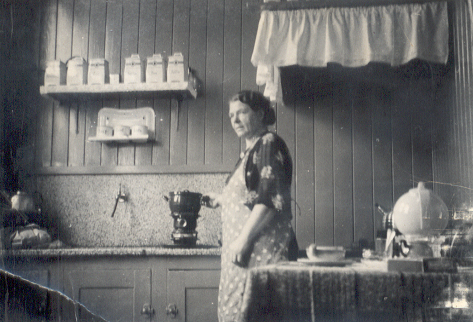
\includegraphics[width=\textwidth]{img/omaJasykofstr}
\caption{Oma Meijns in de Jasykoffstraat}
\end{figure}

Ome Jaap Duif was al overleden. Ik logeerde daar wel eens hoewel mijn vader in onmin met zijn vader leefde vanwege de kwestie van de sigarenzaak (Zuiddijk) die opa aan één zoon (Ome Cas) had overgedaan en de rest van de kinderen had buiten gesloten. Dat zat dus niet lekker. 

Ik heb altijd gedacht dat dat te maken had met de communistische overtuiging van mijn vader. Dat speelde later wel een rol tijdens de Russisische overval op de Hongaren in 1956. Het is nooit een zonder meer hartelijke familie geweest. Het was nooit vechten, schreeuwen of zo, maar wel bedekt wantrouwen. Dat had natuurlijk alles met de sigarenzaak van opa Meijns te maken. De zaak zat niet in de toekomstige erfenis omdat opa hem onderhands had overgedaan aan ome Cas, de oudere broer van mijn vader, zonder de andere kinderen daarin te kennen. 

Opa leek op Drees. Een klein gedrongen mannetje, ook zo’n snorretje. Hij had een aantal wandelstokken met ijzeren plaatjes van plekken waar hij had gewandeld, meestal in Duitsland/Zwitserland.

We gingen als gezin niet veel meer met ze om vanwege ‘de kwestie’. De keren dat ik er logeerde waren wel aardig, ik had geen weet van de problemen. In Het Volk, dagblad, vond ik advertenties van opa en nieuwjaarswensen voor 1930. Ook schreef hij een ingezonden stuk waarin hij tegen het misbruik van alcohol op een partijcongres ageerde.

\emph{Foto: vlnr achter, moe, tante Lena, ome Cas, tante Nel en tante Riena. Zittend Pa met Harry, Oma en opa Meijns en voor Gerard, Elly Berends en Jaap. Harry is nog klein dus voor de 2e WO.}

Achteraf heb ik ook geen idee meer waarom ik ging logeren. Ik sliep boven in een logeerkamertje, direct onder de pannen, met een lampetkan op een kastje met een ovale spiegel en een eigenaardig luchtje (kamfer?). 

’s Morgens ontbijt, tafel met een zeiltje en opa at 1 broodje, maar hij vertelde altijd dat hij er twaalf at. Dat was omdat tante lena het ene broodje in twaalf kleine stukjes sneed. Iedereen ging achterom, eerst de steeg in, dan langs de fam. Vonk, met zo’n kefferig hondje die als hij de kans kreeg je probeerde aan te vallen, maar als je schreeuwde in elkaar kromp, en dan kwam je via de keuken binnen bij tante Lena achter. Het geheel werd omgeven door de oude huishoudschool en de houten wasserij. 

Nooit kunnen denken dat ik later nog eens in dezelfde straat, er recht tegenover zou wonen en de sloop van dat hele blok zou meemaken.

Ik kan me ook nog een ouderjaarsavond herinneren met alle families; die van ome Cas, tante Nel en dochter Carla, van tante Riena, ome Roel en kleine Roel en tante Lena, (ome Jaap?) en onze ploeg. 

Op de TV (1 kanaal) was een ‘Ballet der Lage Landen’, waarop ome Roel zei dat het waarschijnlijk een ballet der lage handen zou zijn. Ik geloof dat de ruzie toen min of meer was bijgelegd, maar helemaal goed werd het nooit. 

\emph{Roel Berends, moe, tante Riena, Janny, Harry, ik, man van Gre, ome Roel, tante Nel, ome Cas, Carla en tante Lena.} 


\chapter{Opa Meijns} % (fold)
\label{cha:opa_meijns}

Ik heb mijn grootvader slecht gekend. De oorzaak is dat ik een nakomertje ben, geboren in 1946. Mijn broers geboren resp. in 1930 en 1937 hebben mijn opa veel langer meegemaakt. 
De ‘kwestie’ was al aanwezig toen ik ter wereld kwam en is maar langzaam een beetje naar de achtergrond verdwenen, maar tegen die tijd waren oma en opa Meijns al overleden.
De ‘kwestie’ gaat over een erfenis, waarom ook niet. Opa Meijns had een sigarenzaak aan de Zuiddijk tussen kapper Leering en banketbakker Landsaat. Achter het dijkhuis lag een grote lap grond met daarop een zaaltje dat werd verhuurd en soms als onderduik werd gebruikt tijdens de 2e WO. 
Toen opa met pensioen wilde gaan heeft hij met z’n oudste zoon Cas een overeenkomst gesloten waarbij hij de winkel en toebehoren aan hem overdroeg in ruil voor gratis huisvesting in de Jasykoffstraat. (Dit alles volgens de overlevering). De andere kinderen bleven buiten de regeling en dat zette kwaad bloed. Mijn vader ging niet meer naar zijn vader, hoewel ik nog wel een aantal keren bij ze op bezoek ben geweest. Ik heb dus een eenzijdig beeld van mijn grootvader.

\emph{Een trouwjubileum (40 of 50 jaar) van opa en oma Meijns. Vlnr: achterste rij: ome Jaap Duijf, tante Nel Meijns, tante Rina Berends, Gerard Meijns (pa), Lena Meijns (ma), ome Cas (van Nel) en tante Lena Duijf (van Jaap.
Daarvoor: Gerard Meijns, Jaap Meijns (van Cas en Nel) en Ellie Berends (van Rina en Roel Berends)
Daarvoor: oma Meijns, (kleine) Roel Berends, opa Meijns en Harry Meijns. Grote Roel is afwezig, was kapitein en waarschijnlijk is dit in de 2e wo. en zat hij op zee.
}

\emph{Met opa en oma voor het huis in de Jasykoffstraat.
}

Door mijn gesnuffel in de Zaanse geschiedenis ben ik toch wat meer te weten gekomen over m’n grootvader. Hij was een actief lid van de S.D.A.P. (Sociaal Democratische Arbeiders Partij) en van de Geheelonthoudersbeweging.

De eerste keer dat ik hem plotseling gewaar werd was toen ik in één van de boekjes “Zaandammers….kent u ze nog?” zat te bladeren. Zie ik opeens m’n opa op de foto met de plakploeg van de SDAP tijdens de verkiezingen van 1925. 

In die turbulente jaren waren de plakploegen ook verantwoordelijk voor het kalken op straat. Het werd zelfs zo erg dat er in de gemeenteraad vragen over werden gesteld. Sommige straten stonden zo vol dat het wel leek of het gesneeuwd had.

Toen ik gevraagd werd het boek \emph{Averechts} van Erik Schaap te recenseren kwam ik m’n opa weer tegen. 

Hij had de hoofdpersoon in dat boek enige tijd onderdak verleend in het gebouwtje achter z’n huis. En jawel, daar stond het “bij sigarenwinkelier Meijns”. Daar had hij de laatste twee maanden van de oorlog ( ’40 -‘45) doorgebracht.

1925 – De plakploeg van de SDAP. Opa achter het bord met hoed.
In de loop der tijd heb ik steeds meer gevonden. Hij was van vele verenigingen voorzitter of bestuurder. Hier nog wat foto’s die ik vond. 
Dat hij muzikaal was blijkt ook weer uit een foto waarop hij, samen met ome Cas met een instrument afgebeeld staat. Aan de bebouwing te zien is het in de Ds. Baxstraat. Recht vooraan in het midden. Ome Cas, 2e rij van boven, 4e van rechts. 

Dit is een foto met het muziekkorps ‘Voorwaarts’ in 1935 op de foto in het Volkspark. Hij zit 1e rij, 6e van rechts achter de trommelaars.

Hij staat uiterst rechts vooraan op de foto als voorzitter van de Geheelonthouderszangvereniging De Korenbloem. Ze staan op de Burcht voor Café Zaandam. Mooie plek voor geheelonthouders.

Ook vond ik advertenties zoals deze uit 1939 waarin 
een ‘Net meisje’ wordt gevraagd.

En op de foto uit 1931 staat hij rechts vooraan als voorzitter van het revuegezelschap ‘Voorwaarts’ voor het station Zaandam. Ze waren op weg naar Amsterdam. Dat geeft toch weer een ander beeld van iemand. Volgens mijn schoonzuster Nel was Gerard, mijn oudste broer, zeer gesteld op opa en oma en ging vaak, met z’n verloofde, bij hem langs. 

Nieuwjaarswens in het Zaans Volksdagblad van 30-12-1939.

Hij deed ook werk voor de geheelonthouders en vocht, in de krant, een debat uit met partijgenoten en tegenstanders die hem nogal radicaal vonden. Hier het afsluitende stukje van de polemiek die 1930 in de krant Het Volk gevoerd werd naar aanleiding van opa’s opmerkingen aangaande drankgebruik. 

Bij de controverse tussen mijn vader en zijn vader zal de politiek mede een rol hebben gespeeld. De strijd tussen de sociaal democraten en communisten is al een hele oude. Begin van de 20e eeuw is die splitsing, vanuit het gezamenlijke begin in de Sociaal Democratische Bond, tot stand gekomen en heeft altijd voort geduurd. 

Zoals gebruikelijk is ter linkerzijde, heeft men elkaar te vuur en te zwaard bestreden en dat zal in de verhouding tussen vader en zoon niet anders zijn geweest. Zoals altijd bij een ruzie tussen volwassenen, zijn de kinderen meestal de dupe. Het is niet anders, maar ik ben toch blij dat ik dit allemaal heb gevonden.

Ik kan me nog wel bezoekjes aan tante Riena en ome Roel herinneren. Tante Riena was een zuster van m’n vader. Ome Roel was zeekapitein en een zeer markant figuur. 

Hij kon vertellen of het nu verhalen dan wel moppen waren, als hij ze vertelde dan waren ze goed. Volgens mijn moeder was het daar altijd net de zoete inval. Als ome Roel thuis was, was het feest. De Gedempte Gracht waar ze woonden, had toen nog gescheiden rijwegen en een plantsoentje in het midden. 

\emph{Bij de foto staat ‘huisje Bakkum’. V.l.n.r.achterste rij: opa en oma Meijns, tante Lena (Duif), tante Nel, Ome Jaap Duif, onbekende. Voor moe en pa Meijns, Gerard/Harry ? en ome Cas.
}

\emph{Op deze staat m’n vader uiterst links, tegen het hek.}

\emph{Dit is het Vermaningspad in 1910. Later is het bestraat. Rechts is het kerkhof. In het 1e huisje links met het puntdak woonde de fam. Kriek. Twaalf kinderen zijn er geboren en grootgebracht. Op de foto hieronder staat Lena links, achterste rij.}

\chapter{Familie Kriek} % (fold)
\label{cha:familie_kriek}

Met de familie van mijn moeder, de Krieken uit Krommenie, ging het veel beter. Daar werd nog wel eens op een zondagmorgen een bezoekje aan gebracht. 

Met de fiets, ik achterop in het zitje, langs de Zaan naar het Vermaningspad, helemaal aan het eind tegenover de begraafplaats. Soms gingen we met de bus. Dan zag je de hele Zaanse industrie langs komen. We stapten uit bij het Badhuis aan de Padlaan. 

Meestal waren ook de andere kinderen, ooms en tantes met aanhang, op zo’n zondagmorgen aanwezig en natuurlijk ome Piet die nog thuis woonde. 

Opa en opoe Kriek hadden, net als ik nu, vaste plaatsen, allebei aan een kant van de tafel die voor het raam in de achterkamer stond en uitkeek op de achterplaats. 

Opa zat links voor het raam en had achter zich een pijpenrekje met diverse pijpen en een rekje voor de krant. Opoe zat links naast de deur naar de keuken.

Op het erf stond naast de werkplaats van opa een houten WC die boven de sloot loosde, met krantenpapier afvegen. 

Je zat met je kont in een open gat en onder je was de sloot, simpel. Vooral bij zware bommen kon het voorkomen dat de plons zo hoog kwam dat ie je billen raakte. 

\begin{figure}[t]
\includegraphics[width=\textwidth]{img/...}
\caption{Opa komt hier net aangereden}
\end{figure}

Opa was, wat je nu, loodgieter, zou noemen, maar toen was het nog een blikslager. Er stond volgens mij nog een handkar op het erf. Je kwam achter binnen via het keukentje waar een aantal oliestellen stonden, dan een opstapje naar de woonkamer. 

In de voorkamer, de pronkkamer, stond een mooi dressoir met daarop foto’s van de ooms als worstelaars en de prijzen die ze hadden gewonnen. De mooiste foto was natuurlijk die waar ze allemaal opstonden met hun prijzen. Op de foto vlnr. Louis, Cor, Frans en Fred.

Boven waren de slaapvertrekken. Het was eigenlijk 1 grote ruimte die in het midden afgescheiden was door een gordijn. 

Toen alle kinderen nog thuis woonden sliepen de meisjes aan de ene en de jongens aan de andere kant. Aan de voorkant van het huis zaten buiten spionnetjes gemonteerd, spiegeltjes waarmee je van binnenuit de hele straat kon afkijken of er iemand aankwam. 

\begin{figure}[t]
\includegraphics[width=\textwidth]{img/...}
\caption{In de bakfiets met Annie, Lena, Rieka, Siema, Jo en opa Kriek}
\end{figure}

Toen opoe begon te dementeren zat ze vaak in een stoel voor het raam te kijken of er iemand kwam. Ze zat dan meestal te wachten op ome Jan, haar oudste, die thuis moest komen voor het eten. 

Ze zette dan ook nog wel eens eten op, maar er kwam nooit meer iemand eten. Eén keer had ze het zo hoog opgezet dat de oliestelletjes begonnen te loeven zodat het hele keukentje zwart was en we nog zijn wezen schoonmaken en witten. Maar toen herkende ze mij al niet meer. Ik kwam er te weinig.

\begin{figure}[t]
\includegraphics[width=\textwidth]{img/...}
\caption{Op bezoek met de familie bij Opoe Kriek. Ze keek altijd een beetje stuurs.}
\end{figure}

Onderling kwamen de broers en zussen nog regelmatig bij elkaar. De band was bij de Krieken hechter dan bij de Meijnsen. Bij zo’n zondags ritje, meestal op de fiets, van Zaandam naar Krommenie ging je de Zaanstreek door via allerlei geuren. 

In de Koog had je Honig, Wormerveer Crok en Laan en in Krommenie had je de Lum ofwel de Linoleum fabrieken en aan het Vermaningspad lag de Blikfabriek. 

Als je blind zou zijn geweest zou je aan de geur weten waar je ongeveer was. 

\begin{figure}[t]
\includegraphics[width=\textwidth]{img/...}
\caption{Opoe en Opa Kriek uit de bios weer naar huis. Ze hadden vaste plaatsen zegt een bron.}
\end{figure}

\begin{figure}[t]
\includegraphics[width=\textwidth]{img/...}
\caption{Moeder en dochter op het achtererf. Zie maar hoe een klein hokje het huis was.}
\end{figure}

\begin{figure}[t]
\includegraphics[width=\textwidth]{img/...}
\caption{De gezusters: Lena, Sima, Rieka, Annie en Jo (en Opoe)}
\end{figure}

\chapter{Mijn ouders} % (fold)
\label{cha:ouders}

Mijn vader vertelde dat hij in Culemborg geboren was. Waarom die uithoek is mij nooit duidelijk geworden. Mijn moeder is in Krommenie geboren. De eerste vrouw van mijn vader en de moeder van Gerard, overleed al heel jong. Ik heb wat foto's bij elkaar gezocht uit hun jonge jaren, voor het beeld.

\chapter{Rosmolenstraat 88} % (fold)
\label{cha:rosmolenstraat}

\begin{figure}[t]
\includegraphics[width=\textwidth]{img/...}
\caption{(de buurt is in 2009 gesloopt)}
\end{figure}

De Rosmolenstraat 88 was een benedenhuis, voor- en achterkamer, 2 slaapkamers, keuken, lange gang en een behoorlijke tuin. De bovenburen hadden geen tuin en ook geen recht op de onze. 

Toen de verhouding met de bovenburen slechter werd en er ruzie ontstond eindigde dat toen ze uit frustratie de pispot in de tuin gooiden. Toen ze verhuisd waren kwamen er Amsterdammers wonen die vreselijk luidruchtig waren vooral als ze samen ruzie hadden. 

Toen mijn vader daar een keer iets van wilde zeggen was het raak. Pa sprak in de deuropening tegen de buurman die boven aan zijn trap stond. Plotseling trok die een touw los waarmee de fietsen tegen de trap vast stonden die met geraas naar beneden kletterden. Mijn vader greep me nog snel en trok hun voordeur dicht die nu, van binnen geblokkeerd werd door fietsen. Ik ben die kleine.

Het was een blok van vier woningen, 2 onder en 2 boven, dat ingeklemd lag tussen de Poortstraat en de Jan Bouwmeesterstraat. Onze achterkant lag tegen de tuinen van de Poortstraat aan. Ik herinner me meer wat achter het huis lag en de uitgang naar de Poortstraat. 

Niemand van de familie kwam via de voordeur thuis, alles ging achterom, de steeg in langs de schutting van onze buren, van der Schaaf, door de poort, langs de heg van buus de Jong en je was achter op het erf. 

\begin{figure}[t]
\includegraphics[width=\textwidth]{img/...}
\caption{Met Gerard achter het huis.}
\end{figure}

Daar hadden we een tuin, stond een schuur, duivenhok, later kippenhok en veel later nóg een schuur voor de fietsen en brommer(s). 

Als Harry thuis kwam dan vlogen de duiven hem al tegemoet. 
Later zijn ze nog jammerlijk aan hun einde gekomen. Geslacht door de schillenboer. Hoe die slachting ooit besloten is blijft in de familiegeheimen besloten. Gerard(?), Harry en ik stonden achter het gordijn naar die slachting te kijken. Ik vol afschuw en fascinatie, iemand die zomaar de koppen van de duiven afsneed en ze in een zak gooide.

\begin{figure}[t]
\includegraphics[width=\textwidth]{img/...}
\caption{Met Harry}
\end{figure}

Later werden ze gebraden op tafel opgevoerd maar niemand moest er natuurlijk iets van hebben. Alles zinloos. 

Het kippenhok, dat Pa had gebouwd voor z’n baas, Kraaijer had een Zaans motief en moe zorgde voor de kippen vooral als er één gepikt werd en ingesmeerd moest worden. We hebben die kippen in Krommenie gehaald. Op een groot omheind stuk grond liepen honderden kippen en wij mochten uitzoeken (Pa en ik). Ik liep in korte broek en die kippen maar in m’n kuiten pikken. 

Een foto van het Zaanse elftal dat in 1946/47 tegen het Belgische Mechelen speelde. Voorste rij rechts, naast Dirk Kuiper zit Rudie Michel, waar ik naar vernoemd ben, is mij verteld. Hij was ZFC’r. 

\begin{figure}[t]
\includegraphics[width=\textwidth]{img/...}
\caption{Zelfde karretje als dat met Harry, nu met Peter Baas. Volgens mij dezelfde manteltjes. Ik mocht zeker het karretje niet uit.}
\end{figure}

Naast ons woonde de familie van der Schaaf. Net als wij waren zij communistisch georiënteerd, maar fanatieker dan bij ons thuis. 

De zonen van v.d Schaaf (onze directe buren) werden naar partij-iconen van de communistische wereld vernoemd. Paul naar Paul de Groot, CPN partijvoorzitter. En Karl naar de Duitse communist Karl Liebknecht. 

Omdat mijn vader en vd Schaaf van mening verschilden over het communisme spraken ze niet meer met elkaar. Met de familie boven ons, kregen we later ruzie, waarom is mij niet bekend behalve dat ze rotzooi in onze tuin gooiden. 

Boven v.d. Schaaf woonde de fam. Schaap, met zoon Jaap zat ik in de klas en z’n vader werkte als chauffeur bij Bruynzeel. 

Toen de man een keer even thuis was en z'n truc in de straat parkeerde zei Jaap dat we er wel even in mochten. Door wat voor oorzaak ook startte de auto en reed heel langzaam vooruit. Van schrik sprongen we er beiden uit, maar als held ben ik er weer ingeklommen en pakte het stuur. 

Gelukkig kwam buurman er al aanrennen en nam het over. Maar omdat ik er alleen in zat viel er wel een sterke verdenking op mij. 

Schuin tegenover ons woonde een familie met een thuis-wonende zoon die blindegeleidehonden africhtte. We mochten wel eens mee naar het Oostzijderveld dat aan het eind van de Poortstraat begon. Hij had altijd Duitse herdershonden. Z'n ouders waren al bejaard en als het gordijn weer dichtging wist je dat moeder… weer bediend werd door de pastoor. Meestal gingen de gordijnen na een paar dagen weer open. 

T.o. ons op de eerste verdieping kwam fam. de Licht wonen, met Coby, de mooiste van de straat. Veel gehoelahoept met haar en doktertje gespeeld in een tent achter het huis. Tot we onraad hoorden en een hoofd de tent binnen keek. Zweten en een rooie kop van de spanning. Foto: Kamp Bakkum. 

Dat we communistisch waren betekende niet zoveel voor de buurt behalve in verkiezingstijd. Dan hadden wij een bordje aan de deur hang met rood vlak met daarin een witte 6, van lijst 6. Paul de Groot. 

De Jan Bouwmeesterstraat, de eerstvolgende straat was helemaal katholiek, dus die stemden allemaal KVP. 

Als zij bij ons de bordjes van de CPN eraf sloegen dan loerden wij op een kans om met lange stokken door de Jan Bouwmeesterstraat te rennen om die KVP-bordjes er af te slaan.

Maar normaal was er geen enkele animositeit want de vaders waren als oude vrienden en stonden gewoon met elkaar te kletsen. 

Er werd nog wel eens gekeken of je wel met iemand vriendje mocht zijn. Toen er een nieuwe jongen in de straat kwam wonen moest hij eerst thuis vragen of hij vriendjes met mij mocht zijn, het mocht, omdat ik bij ondervraging kon melden dat mijn vader Gerard Meijns was. “Oh, Geer Meijns”, zei de vader. 

Toen was het goed, ze kenden elkaar. Tja, je weet maar nooit blijkbaar, het was tenslotte Koude Oorlog. In een buurt waar iedereen elkaar kent hoef je nooit voorgesteld of gekeurd te worden, dus dat fenomeen was mij onbekend.

Ik kan me nog herinneren dat ik een keer met Ellie Nijzing uit de Jan Bouwmeesterstraat naar de nachtmis ben geweest. Later werd Ellie de vrouw van Theo Blankesteijn. Wie had ooit kunnen denken dat ik later Theo zou ontmoeten en dus ook weer kennis zouden maken met Ellie. 

Maar goed, ik met de familie Nijzing mee naar St. Bonefatiuskerk in de Oostzijde. Een hele en vooral landurige vertoning en na afloop gingen we eten bij de familie Nijzing thuis. 

Ik heb geen idee hoe men er thuis tegenover stond. Ik ben veel later nog eens met Co Smit naar een kerstmis in Wormerveer geweest. Ik zat met Co in een bandje. Die mis duurde ook te lang naar mijn mening, net als de Mattheuspassie die ook veel te lang is, maar dat terzijde.

Hr. en mevr. Pel hadden in huis een winkeltje in tabakswaren met net zo'n vlammetje op de toonbank als bij m'n ome Cas in zijn winkel aan de Zuiddijk. Door de gang en in het zijkamertje dreven zij hun negotie. 

Maar zij waren ook het huis met een TV. Zo’n enorme kast met een, in verhouding, klein beeld. Niet iedereen had toen TV en je keek bij buren die er wel één hadden.

Dus, zoals bekend uit vele verhalen, woensdag- en zaterdagmiddag TV-kijken met een stel kinderen. Schoenen uit en met z'n allen voor de buis. Ik weet niet of ze er ook iets voor vroegen.

Tante Hanny met de Verrekijker waarin wetens-waardigheden van over de gehele wereld werden getoond. 

Een verhaal met een vliegende Knorrepot, waarbij je de draadjes waaraan hij door de lucht vloog duidelijk kon zien. 

Echt voor kinderen dus. Series als \emph{Morgen gebeurt het}, een spannende toekomstvisie met ruimteschepen etc. Dat was heel spannend, maar als je nu ziet hoe het décor eruit zag, is het niet voor te stellen dat dat eng was.

Er was blijkbaar veel vraag naar verhalen over de toekomst want op de radio was het hoorspel \emph{Monus de man van de maan} erg populair. Ik was daar een grote fan van en had ook een boek van de serie gekregen. Dit boek. De radio was eigenlijk het enige vertier. De hoorspelen waren meestal in het weekend want door de week moest iedereen vroeg naar bed.

We hadden ook een beeldhouwer in de straat. Iets verder als waar wij woonden, daar waar midden in het blok huizen een grote steeg naar achter de huizen leidt. Ik kende de man alleen van in zijn werkruimte die vanaf buiten te zien was. 

Hij houwde beelden voor kerken e.d. en 's zomers als zijn raam openstond kon je hem aan het werk zien. Ik heb hem nooit anders dan in dat kamertje gezien, nooit buiten of zo.

De schillenboer kwam met paard en wagen langs en stopte in de Poortstraat en haalde dan achterom z’n waar op. (en slachtte soms ter plekke). 

\begin{figure}[t]
\includegraphics[width=\textwidth]{img/...}
\caption{Hier zit ik op het paard van de schillenboer.}
\end{figure}

De kolen werden natuurlijk ook achterom gebracht. In het oude schuurtje was de bak voor de kolen. Met een kolenkit haalde je de kolen naar binnen. Later toen we een oliekachel kregen kwam de olieboer met z’n wagentje langs. Hij woonde op het St. Catharijnepad.

De kolen en de olie hebben beiden een aparte geur. Vlak bij school, Herderstraat of zo, was een kolenboer. Op het terrein waren verschillende vakken voor alle soorten kolen die hij verkocht. Ook achter het spoor bij het station waren enkele opslagplaatsen voor kolenhandelaren. De melkboer kwam natuurlijk aan de voordeur.

De Poortstraat was eigenlijk de opening naar de wereld. Door de steeg was je zo bij de Sparwinkel (volgens buus de Jong heette hij Henri), naar vrienden Jan Schoen, Leen Bakker en Peter Baas die in het volgende plantsoen woonde. 

En naar buurvrouw (buus) de Jong natuurlijk. Ik ben er onlangs nog eens langs gereden. Buus de jong woonde om het hoekje en als ze de achterdeuren naar de tuin open had staan en ze hoorde me langskomen kon ze vragen om een boodschap te doen bij de Spar, of vroeg ze of je trek had in iets lekkers, meestal ontbijtkoek, dik besmeerd met (echte) boter. Ze had van dat lange grijze haar in vlechten en was altijd wel een beetje ziek.

Buus hield van poezen en bij haar mocht ik graag vertoeven. Er hing een geur van oude gezelligheid, van dikke kleedjes, sigaren en poezen. Ze had stapels Katholieke Geillustreerde of Het Leven, met veel plaatjes over verre werelddelen, rampen, grootse gebeurtenissen enz. Je kon heerlijk op de grond liggen bladeren en buurman de Jong zei nooit zoveel. 

\begin{figure}[t]
\includegraphics[width=\textwidth]{img/...}
\caption{In de Poortstraat, links de ingang van de steeg en het huis van Buus de Jong.}
\end{figure}

We waren allemaal van Zaanlandia en buurman stond in de kantine en toen mijn ouders hun 25-jarig huwelijk vierden stond hij er ook. Buurvrouw heb ik er nooit gezien ze was altijd wat zwak en ziekjes. 

Vlak bij school had je bakkerij de Zeeuw, pardon een Banketbakkerij. Als je daar de deur open deed kwamen de heerlijke geuren van gebak en fijne allerhande je tegemoet.

Broer Gerard was al jong de deur uit, naar Den Haag waar hij bij de PTT werkte en een opleiding kreeg. Hij was dus al het huis voordat ik me van hem bewust werd. Hij rookte Dr. Duskind, reed op een Vespa (scooter) en had een verloofde; Nel. Ze huurden een kamer in Amsterdam-West.

Onlangs kreeg ik wat fotootjes uit die tijd. Ik ben nog eens met m’n vader op de fiets naar Amsterdam geweest waar ze een etage hadden. 

Hun huwelijksfeest werd gehouden in het Pontrestaurant in Amsterdam Noord waar ik mee mocht helpen met de bediening. Als een echte ober liep ik met het dienblad rond. Als het restaurant niet gesloopt was, zouden ze het er nog over hebben, zo’n succes was dat.

\begin{figure}[t]
\includegraphics[width=\textwidth]{img/...}
\caption{Hier gaan we op weg bij Nel haar huis in Ransdorp.}
\end{figure}

\begin{figure}[t]
\includegraphics[width=\textwidth]{img/...}
\caption{Kijk m’n pinkelhoutje? En natuurlijk korte broek.}
\end{figure}

Wat ik als kind erg spannend vond was met een spiegel door het huis lopen. De spiegel hield ik voor m’n borst en probeerde dan alleen in de spiegel te kijken en door het huis te lopen. Bij de overgang van de kamer naar de gang stapte je dan in een diep gat omdat het plafond in de gang dieper was of leek. 

Het spannendst was om zo eerst een tijdje in huis rond te lopen en aan het kijken in de spiegel gewend te raken en dan de stap vanuit de keuken naar buiten te maken want dan viel je de lucht in. En werkelijk alsof je geen grond meer onder je voeten had zo spannend was dat. Bij de achterdeur naar de tuin was een afstapje. Als je dan met de spiegel liep had je het gevoel steeds verder de hemel in te stappen, heel eng. 

\begin{figure}[t]
\includegraphics[width=\textwidth]{img/...}
\caption{Het afstapje met m’n vader, moeder van Peter en mijn moeder.}
\end{figure}

Als m’n moeder de was deed stond er in het begin een grote wastobbe op het vuur en in de zomer stond ze buiten met het wasbord de kleding te kuisen. Later kwam er een wasmachine of alleen een apparaat dat in de tobbe rond draaide. 

We waren ook lid van speeltuinver. Het Oosten, met een gebouwtje voor films in de Oostzijde. Zaterdag- of woensdagmiddag was duwen en trekken voor de ingang om als eersten binnen te komen want er waren altijd meer gegadigden dan stoelen. Bij de ingang stond een man van de speeltuin om orde te houden. 

Het was een grote man met een klompvoet en een schoen die twee keer zo groot was als z’n andere. De films waren meestal Dikke en Dunne, soms Three Stooges of Comedy Capers of The Keystone Corps (foto). 

In het filmzaaltje was de chaos bijna net zo groot als op het witte doek, veel geschreeuw. Ik weet nog dat in de winter, toen we al heel lang voor de deur stonden te wachten er iemand op m’n voet ging staan en ik de hele voorstelling lang een vreselijke pijn had want mijn voet werd niet meer warm. Na de voorstelling hard naar huis rennen.

Een keer een voorstelling in het Apollo theater gezien van Sjors en Sjimmie in Afrika waar ze het aan de stok kregen met wilden maar ook met krokodillen. Na de voorstelling bleek het buiten al donker te zijn geworden en ik wist niet hoe snel ik thuis moest komen, want je weet maar nooit met krokodillen. Thuis direct naar m’n kamer en met een sprong op m’n bed, voor de veiligheid. 

\begin{figure}[t]
\includegraphics[width=\textwidth]{img/...}
\caption{Het Apollo theater}
\end{figure}

\chapter{Kleuterschool} % (fold)
\label{cha:kleuterschool}

Gelukkig was de kleuterschool dichtbij. Vanuit huis liep ik er in twee minuten naartoe. De man met de kar is Noë van de Poort - kruidenier, later De Spar.

Op de foto van de kleuterklas staat m’n juf, Winsemius, waarmee ik als ik groot zou zijn zou gaan trouwen. 

Jan Schoen zit uiterst links, op het verhoginkje. Peter Baas zit op de tweede rij uiterst rechts en vooraan. Die met het witte truitje is Lyda Hooyschuur en met de zwarte galgjes rechts daarvan zit ik. 

We zullen ongetwijfeld veel knip- en plakwerk hebben verricht. We kijken hier allemaal verrast om. ‘Wat, een foto?’

Een blijvende herinnering is wel dat ik met m’n autoped m’n grote liefde naar huis bracht. Ze was de dochter van de dominee die in de Oostzijde woonde, op de hoek van de Schoolmeesterstraat van de ijsboer \emph{De Danser} en de snoepwinkel waar we ‘bakkesvols’ haalden. 

De poort naar de school was bevestigd aan twee stenen pilaren waar je op kon zitten. Tijdens één van die zittingen heb ik Jan Schoen een gat in z’n hoofd geslagen en hem daarna zorgzaam naar huis gebracht. Waarom is me nooit duidelijk geworden, want het was mijn beste vriend. 

\chapter{Stegen en straten} % (fold)
\label{cha:stegen_straten}

In onze buurten waren de stegen erg belangrijk. Onze eigen buurtstegen waren een bron van veiligheid, omdat je precies wist waar ze naartoe leidden en wat je kon verwachten. Wat verder uit de buurt kon je weleens voor verrassingen komen te staan als je zomaar een steeg instoof. 

Er zijn stegen met onuitwisbare herinneringen, zoals toen ik de melkboer hielp en met flessen onder m’n arm via de Poortstraat de steeg van de Rosmolenstraat inliep en viel. Handen vol glas, waar nog de tastbare bewijzen van zijn te leveren. Of die keer, in dezelfde steeg, toen iemand me tekkelde en ik wel zere knieeën had, maar pas thuis merkte dat m’n broek aan m’n knie zat vastgeplakt van het geronnen bloed. Dat deed bloed toen nog.

En onze eigen steeg, die er recht tegenover lag. Daar zat ik tijdens de dagen voorafgaand aan luilak uitdagend te doen op een autoband die wij al hadden voor het feestvuur, tot een ploeg vanuit de Jan Bouwmeesterstraat plotseling kwam aanstuiven en de band onder m’n kont vandaan trok. Ik kon nog net m’n hand door het gat slaan en keihard om hulp roepen. Bij de kruising van de Poortstraat en het Albert Hahnplantsoen waren er genoeg vrienden te hulp geschoten om het in een vechtpartij te laten ontstaan die door ons werd gewonnen. 

Toen ik onder de kluwen omhoog kwam stond er een ‘vijand’ te lachen ik heb hem toen een kaakslag gegeven als een volleerde boxer.

Kort daarna liep ik op de Heijermansstraat tussen de Poortstraat en Jan Bouwmeesterstraat toen ik plotseling tussen een stuk of tien Jan Bouwmeester-straters stond en met m’n rug tegen de buitenmuur van het laatste huis werd geduwd. Er was geen ontkomen aan en ik kreeg flinke klappen. 

\emph{Heijermansstraat met rechts de de muur waartegen ik de klappen ontving.}

Nog een incident vondt plaats toen een delegatie uit de Jan Bouwmeesterstraat--- naar later bleek versterkt door Rooms-Katholieke-geloofsgenoten uit Brabant---ons te lijf wilden gaan met stokken met voorin een grote spijker. Bij het uitdagen waren wij in de Poorstraat toch weer in de meerderheid en drongen wij de Roomsen een steeg in. Daar, ik moet het bekennen, maakte ik een van de stokken afhandig en duwde die een Katholieke Brabantse buik in. De jongen is nog naar het ziekenhuis vervoerd en er werd niet naar de dader gevraagd. Onze monden voor eeuwig gesloten. Zo hoort dat onder makkers.

Verderop hadden we ook wel vriendjes zoals in de Koning Williamstraat, maar dat was toch al verder dan onze directe buurt. Als je wat groter bent wordt je actieradius ook wat groter. Als je klein bent is een tocht naar een heel andere straat al een hele onderneming.

Wim Al was een vriendje. Hij woonde in de Leo XIII straat. Zijn vader had een transportbedrijf. 

Hij kwam veel in het Veem en vond daar een torenvalkje. Hij bracht het mee naar huis en Wim mocht het opvoeden. Eten geven bedoel ik. 

We gaven het beestje wormen die we eerst door de midden knipten, anders zou het valkje stikken. Dat ging heel goed en op een dag vloog hij weg.

Toen de wereld in de ban was van de eerste ruimtereizen besloten wij ook een poging te wagen. We hadden een kleine raket gebouwd, van hout met vleugeltjes, stopten er spiritis in en lucifers, staken het aan, \emph{woesj!} een kleine vuurbal en hij viel om. Einde ruimtevaartclub.

Toen Olga en ik later met Chris en Kelly in Drenthe vakantie vierden kwamen we langs een uitspanning met een kaboutergrot. Altijd leuk voor de kinderen. Je moest afdalen in de grond en daar was een pad uitgegraven dat je langs allerlei kabouters voerde die aan het werk waren of lagen te slapen. 

Boven gekomen gaan we nog wat drinken, dan hoor ik opeens: ``Hé Ruud Mainz''. Was het Wim Al die de eigenaar van deze uitspanning was. Hij sprak nog steeds Zaans.

\chapter{Wat er door de straat kwam} % (fold)
\label{cha:straat}

De straat had nog het karakter van een openbare marktplaats. Van alles probeerde de waren huis aan huis te slijten: de melkboer, groentenboer, schillenboer, visboer, ijsboer, voddenman, ambulante handelaren \emph{und so weiter}. 

Onze melkboer was Langelaar, die in onze straat z’n winkel had. Met z’n karretje verkocht hij losse melk die zo in een pannetje of in flessen geschonken werd. 

Ik mocht hem helpen en na z’n wijk te hebben gedaan moesten alle melkbussen en dergelijke schoongemaakt worden. 

\begin{figure}[t]
\includegraphics[width=\textwidth]{img/...}
\caption{Garage van Langelaar}
\end{figure}

Dat gebeurde in z’n garage met heel veel water. 

Met dat helpen heb ik me nog eens aardig bezeerd. Ik liep met de flessen van de kar achterom een steeg in en kwam terug met lege flessen. Achter een heg zat iemand met een stok die tussen m’n benen werd gestoken. Ik viel voorover, strekte m'n handen om de val op te vangen vol in de gebroken flessen. Allemaal glas in m'n handen en een kapotte knie.

Van een groentenboer kan ik me niet zoveel herinneren. Van de aanverwante schillenboer meer, omdat die met een paard en wagen langs kwam. 

Ik sta nog op een foto met dat paard, genomen vanuit de Poortstraat. De visboer kwam, voorafgegaan door z’n vrouw Marie op haar fiets, met de bakfiets door de straat. Zoals veel ambulante handel had Marie een kreet waardoor je van ver al wist dat de visboer eraan kwam. Ze had nog een ouderwets soort kleding aan met veel schorten over elkaar.

De voddenman, een klein gedrongen mannetje, kwam ook op de bakfiets en een eigen kreet de straat in. Je verstond er niets van, maar je wist `dat is de voddenman’. Hij had een pakhuis in de Zilverpadsteeg waar we als kinderen ouwe kranten konden aanleveren. Het was net een hol waar je binnenkwam. Het hing en stond vol met spullen. 

Er waren ook handelaren die de ene keer met dekens en dan weer met een kar vol met fruit langs kwamen. Ik heb ook nog meegemaakt dat een man met garen en band langskwam; een echte marskramer. En natuurlijk de ijskarren die je al van ver hoorde aankomen. Als je al in bed lag maar hopen dat er toch nog een ijsje zou komen.

De ijsboeren waren een slag apart. Je had `de danser’ uit de Schoolmeesterstraat en die van ijssalon \emph{Tempo} in de Damstraat. 

De eerste werd `de danser' genoemd omdat hij door het gewicht van z’n ijskar, als die nog vol was, omhoog geduwd dreigde te worden en z’n kracht dus op het neerdrukken moest richten. Hij kon als het ware zwevend lopen. 

\begin{figure}[t]
\includegraphics[width=\textwidth]{img/...}
\caption{IJszaak Tempo}
\end{figure}

Tempo was een echte Italiaan met dito ijs. Zijn zaak in de Damstraat was vooral bekend door als startpunt te dienen voor het geflaneer van de opgeschoten jeugd.  Die gingen vanuit daar richting de Westzijde, ongeveer tot aan het Typhoongebouw en weer terug. Dat werd ook wel ‘billenavond’ genoemd. 

\chapter{Luilak} % (fold)
\label{cha:luilak}

Luilak was sowieso een fantastische tijd waar veel over te vertellen valt. Als je klein bent loop je met je vader, broers en zijn vrienden, buren enzovoorts mee. Op elk kruispunt was wel een fik. Als je groter wordt ga je het zelf doen met leeftijdgenoten. 

Meestal was de gezelligheid vooral de tijd die eraan vooraf ging: het verzamelen. 

Bij elke deelnemer aan een fik werd van alles opgeslagen, tot de dag daar was en het op de plek van ontsteken werd bijeengebracht. Spannend was natuurlijk wie de grootste fik had. Als het te groot was kon je last krijgen met de politie.

De grootste fik in mijn jonge jeugdjaren was het vuur op het grasveld voor de Noorderkerk, dat zo groot was dat het het grote, ronde, gebrandschilderde raam dreigde te smelten. Onze dienders hadden het maar druk met al het kattekwaad. 

Ik ben één keer opgepakt toen ik een motor in de brand had gestoken. Lang verhaal, maar er zat benzine in en dat wilden we aftappen. Af en toe staken we hem een beetje in brand en bliezen het weer uit tot het niet meer uitging door alle gemorste benzine. Toen het duidelijk was dat het niet meer te blussen was vloog iedereen weg. 

Ik kwam thuis en vertelde m’n ouders van de fik. M’n vader zei: ``Ga maar terug en kijk hoe het ermee staat, dat kun je niet zo laten gaan,'' of iets in die geest. Ik weer terug en iedereen was weer terug. Toch proberen hem uit te maken en plots stond er politie. 

Na veel vragen ben ik naar voren gestapt en heb me aangegeven als de aanstichter. De motor werd in een zandwagen geladen en ik met de chauffeur (geen politie) naar het politiebureau. 

\begin{figure}[t]
\includegraphics[width=\textwidth]{img/...}
\caption{Het politiebureau in de Vinkenstraat (nu weg).}
\end{figure}

Onderweg naar het bureau zei de chauffeur me niets te bekennen en vol te houden dat het een ongeluk was. Op het politiebureau zat ik in het wachtlokaal en hoorde alle oproepen om bijstand als er een geasfalteerde weg begon te smelten. Met mij deden ze niets. Lieten me alleen zitten. Uiteindelijk werd ik door m’n vader pas om acht uur opgehaald en de volgende dag als een verzetsheld door de vriendjes begroet. 

De eigenaar van de motor is nog langs geweest om via de verzekering iets te regelen. Hij noemde zijn naam, `Kattestaart', wat thuis tot veel hilariteit leidde.

Met luilak kon je ’s morgens al heel vroeg bij de bakker warme witte bollen kopen. Ik dacht altijd dat hij dan speciaal voor luilak zo vroeg open ging, maar hij was natuurlijk allang aan het bakken en deed alleen z’n winkel vroeger open. 

\chapter{Vreemde zaken} % (fold)
\label{cha:vreemde_zaken}

Er was een oude man in de Tolstraat die zich vanwege een handicap in een (nu) antieke rolstoel moest voortbewegen. Twee stangen dreven het apparaat vooruit. Je moest ze met de hand op en neer duwen. De bochten waren het moeilijkst, leek me, als je vaart moest houden en tegelijkertijd een bocht moestnemen. Ik heb er altijd met fascinatie naar gekeken. 

Dat kijken vond mijn moeder wel eens hinderlijk. Elke keer als we op straat iemand met een handicap tegen kwamen bleef ik daar gefascineerd naar kijken. Soms deed ik het ook na, waarop mijn moeder dan me beschaamd toeriep om met die onzin te stoppen. Ik kon naar elke handicap blijven kijken.

In de Rosmolenstraat woonde een mevrouw die een krop had. Die persoon had dan een soort ballon in de nek hangen. 

Tegenwoordig zie je dat niet meer. Je ziet sowieso geen handicaps meer die vroeger normaal waren om tegen te komen. Er zijn veel meer mogelijkheden om foutjes van de natuur vroeg op te sporen en er iets aan te doen.

Mensen die slepen met een klompvoet. Eén voet normaal en de andere voorzien van een enorme schoen. Die mensen liepen altijd ongelijk. Ik heb zo’n leraar gehad.

In de Kopermolenstraat woonde een meisje, Beppie. Ze was klein, kleine handjes en voetjes en had een waterhoofd. Ik ken haar alleen maar als zittend in de deuropening met een schare kinderen om haar heen. Ze was niet mentaal gehandicapt, want ze kon goed met de kinderen om haar heen overweg. Maar dat hoofd, ik kon m’n ogen er niet vanaf houden.

\chapter{Sport} % (fold)
\label{cha:sport}

Eén van m’n vroegste sportherinneringen is het kladetsen. Twee deelnemers zijn meestal genoeg. De broek, in ons geval een korte gebreide broek met eveneens gebreide houders over de schouders, moet uit. Het kladetsen doe je door elkaar op de billen te slaan. Na een tijdje wissel je van plek. 

Toen we zo’n tijdje in de tuin bezig waren werden we gemaand hiermee te stoppen. Ik denk dat we een jaar of drie waren. Later deden we het nog in het In ’t Veldpark.

Laatst dacht ik nog over de mooiste doelpunten die ik heb meegemaakt, naar aanleiding van een tv-uitzending. De mooiste waren de doelpunten bij ZFC thuis.Ook als je als kind speelde en niet keek en er steeg plotseling zo’n storm van geluid op dan kwam er zo’n heerlijk vreugdevol gevoel over ons allen. \emph{We} maakten een doelpunt en \emph{we} waren blij. In het seizoen 1958 werd ZFC kampioen van de Tweede divisie.

Mijn vader was een ZFC’er en ging de thuiswedstrijden altijd kijken. Hij had een vaste plaats op de staantribune achter het doel aan de kant van de Westzanerdijk. 

De kinderen speelden rond het terrein. We probeerden dan gratis op de tribune te komen. Iemand gooide dan het kaartje langs de kant naar beneden en zo kregen we dan soms toegang. 

\begin{figure}[t]
\includegraphics[width=\textwidth]{img/...}
\caption{Het ZFC-veld, we kijken naar de staantribune aan de Westzanerdijk.}
\end{figure}

Onder de staantribune vonden we nog wel eens iets wat de mensen daarboven hadden laten vallen. Mijn vader kon ontzettend hard schreeuwen. Je kon hem overal bovenuit horen. Als de familie (pa, moe en ik) het terrein op kwam werd er op de staantribune al plaatstgemaakt door de vaste groep. Moe ging alleen mee als het lekker weer was. 

Als het afgelopen was moest je eerst je fiets weer terugvinden. Die stonden in lange rekken op de Westzanerdijk. Daarna ging die grote slinger weer terug naar huis, veroorzaakte opstoppingen bij de smalle Wilhelminabrug. Naarmate de tocht naar huis vorderde, werd de groep steeds kleiner. 

Van m’n sportcarrière bij Zaanlandia weet ik nog enkele flarden. Bijvoorbeeld de wedstrijdjes bij de welpen, waar elk team de naam van een beroemde voetbalclub had (wij waren Barcelona) en we op een half veldje speelden. Dat was nog op het oude Zaanlandia terrein, met sloten er omheen, tegenover de Veeringstraat. Later kwam daar een verpleeghuis, en nu staat daar grotendeels het ziekenhuis.

Bij de aspiranten---ik zat in de F-jes---weet ik nog van een wedstrijd tegen ZFC op het B-veld aan de Westzanerdijk. Ik was altijd rechtsback, maar toen had ik een \emph{rush} naar voren. Omdat het veld zo groot was, had ik toen ik eindelijk in de buurt van het doel van de tegenstander kwam geen kracht meer om de bal er fatsoenlijk in te schieten. En daarna helemaal terug naar je eigen plek, weer dat hele veld over. 

Soms moest je ook heel ver uit spelen. Een keer, bovendien de laatste keer, speelden we bij een club aan het eind van Krommenie, aan de Provinciale weg. Op de fiets gingen we er heen, voetballen, en weer op de fiets terug. 

Toen ben ik maar op judo gegaan. Ik speelde bij Judoclub Zaandam, onder leiding van Siem Boering. Een strenge trainer, maar wel een goeie. Als hij zag dat je je voor een wedstrijdje met hem terug trok, dan haalde hij je eruit. Nooit terug trekken, vond hij. En terecht. We trainden in de Wilhelminaschool, aan de Gerhardstraat. Op die plaats staan nu woningen.

Eénmaal heb ik in een wedstrijdteam in Amsterdam gejudood. In die partij kwam het tot een eindgevecht op de vloer, waarbij ik m’n tegenstander in de derde houtgreep kreeg. Altijd lastig. Dan duren die zestig seconden heel lang om hem erin te houden. Je ziet in een ooghoek je teamleden springen en schreeuwen en die man onder je licht te kronkelen om eruit te komen. Maar ik heb hem wel eronder gehouden. 

Zwemmen heb ik geleerd in de vierde klas. Mijn moeder stond dan bij school te wachten en uit school gingen we rechtstreeks naar het Sportfondsenbad in de Mauvestraat. 

Dat was ook het bad waar we schoolzwemmen kregen. Het was een mooi bad, maar de kleedhokken beneden waren nat en koud. Ik vond het smerig daar, maar dat terzijde. 

De eerste lessen krijg je met een haak om je buik. De zwemleraar---de vader van een klasgenote--hielp e door de eerste fase heen. Bij het alleen zwemmen kreeg ik krampen. Volgens de badmeester aanstellerij, maar toen dat maar aan bleef houden toch maar eens door de huisarts laten onderzoeken. Navelbreuk. Dus lag ik voor een operatie in het ziekenhuis en heb daarna nooit meer last gehad.

Ik lag een week, of misschien veertien dagen, in het ziekenhuis. Daar lag ik met nog een jongen op een apart kamertje, terzijde van de mannenafdeling. Toen ik weer mocht lopen ging ik de zaal op en kreeg nogal wat snoep toegestopt van de mannen daar. Goeie tijd gehad.

Toen ik thuis kwam kreeg ik, voor alle ontberingen, een voetbal. Geen echte van leer, maar iets wat er op leek. We zaten met z’n allen in de achterdeur naar de tuin met de voeten op het trapje. De bal werd uitgepakt, er werd wat meegespeeld en hij sprong af op een spijker en dat was het kado---lek. 

Nog een pechgeval. Op een verjaardag kreeg ik een keer van Jim, de Ierse echtgenoot van Elly Berends, een zeilboot om in elkaar te zetten. Omdat er op verjaardagen meestal niet veel te doen is, besloten Gerard en anderen de boot alvast in elkaar te zetten. Trots werd mijn kado als ‘klaar’ gepresenteerd. Daar had ik in ieder geval niet veel meer aan.

Als je wat ouder en wat wilder wordt gaat het wel eens mis. Zo ben ik eens tijdens een spelletje tikkertje van de hoge duikplank afgedonderd. Niet van de plank in het water. Nee, ik miste een tree bij het beklimmen van de trap, viel terug en klapte met m’n hoofd op het beton. 

Ik ben bewusteloos geweest en toen ik bijkwam was het een oorverdovend lawaai van schreeuwende kinderen. Naar het ziekenhuis in de Frans Halsstraat gebracht en daar behandeld.

Mijn begeleiders waren alweer vertrokken, zodat ik toch nog met een hersenschudding op m’n fiets weer naar de Rosmolenstraat terug moest rijden. Daar moest ik prompt overgeven. 

\chapter{Het oude ziekenhuis} % (fold)
\label{cha:ziekenhuis}

Toen ik een andere keer van het zwemmen naar huis reed kwam ter hoogte van de Jedelooschool en de toenmalige groentenboer m’n badtas tussen m’n voorwiel en dook ik over m’n stuur met m’n kin op de straatstenen. En zeer dat m’n kin deed. Pas toen de groenteman naar buiten kwam en me overeind wilde halen merkten we pas dat m’n kin open lag. Weer naar het ziekenhuis en krammetjes erin. En weer alleen op de fiets naar huis.

Bij het ziekenhuis stond de kraam van Cor Knikker. Cor had een lamme rechterhand. Als mijn moeder zag dat ik weer een lichaamsdeel met een elastiekje afknelde hield ze me voor dat Cor zo ook aan z’n verlamde hand was gekomen.

\begin{figure}[t]
\includegraphics[width=\textwidth]{img/...}
\caption{Cor met z'n lamme rechterhand}
\end{figure}

We hielden eens een wielerwedstrijd rond de Rosmolenstraat en de Koning Williamstraat. In een bocht vlak voor de kleuterschool, bij het huis van Lyda Hooyschuur, gleed ik door zand onderuit en belandde in het hek met prikkeldraad. Toen ik m’n arm eruit haalde kon ik zo naar binnen kijken. Weer naar ‘t ziekenhuis. Nog steeds is deze plek te bewonderen op m’n bovenarm. 

Dat wielrennen heeft wel een tijdje mijn belangstelling gehad, omdat mijn vader bij de Zaanlandse wielerclub DTS wat prijzen had gewonnen. Toen hij eens met een baanstuur voor mijn fiets thuiskwam was het einde natuurlijk zoek. Overal waar ik heen reed deed ik dat met de grootste spoed. Alles moest snel. We deden ook aan tijdrijden. Van ons huis in de Rosmolenstraat via de Heijermansstraat naar de Paaskerk en weer terug.

Bij de Paaskerk was Karel Appel net aan het schilderen en zag ik Freek de Jonge nog lopen. Hij zou er later uitvoerig over schrijven, maar mijn recordpoging heeft hij over het hoofd gezien. 

\begin{figure}[t]
\includegraphics[width=\textwidth]{img/...}
\caption{Karel Appel in de paaskerk}
\end{figure}

Zoals Freek in zijn boek ook mijn aanwezigheid bij de brand in het Veem aan de Oostzijde onvermeld liet. De grootste brand die ik ooit gezien heb. We kwamen allemaal te laat op school. 

\begin{figure}[t]
\includegraphics[width=\textwidth]{img/...}
\caption{De foto is vanuit de Hoveniersstraat genomen.}
\end{figure}

We woonden vlakbij het Veem en in het Konijnenpad en de Hoveniersstraat had je een goed uitzicht op de brand. De Zaan stond door de cacaoboter in brand. Harry, die bij Sabel werkte, had een goed overzicht en zag de panden instorten en de Zaan in brand staan.

Wij moesten weer naar school. Ik sprak laatst een oud brandweerman en die vertelde nog met liefde over de mooiste brand die hij ooit had meegemaakt. 

\chapter{IJspret} % (fold)
\label{cha:ijspret}

Ik heb als kind altijd veel geschaatst. Vooral op de Gouw, die toen de voor geoefende rijders een uitvalsbasis was naar verre oorden, zoals Marken.

\begin{figure}[t]
\includegraphics[width=\textwidth]{img/...}
\caption{Brug over de Gouw.}
\end{figure}

Toen in 1960 Tuindorp/Oostzaan overstroomde kon je er op de schaats gaan kijken. Omdat Harry en z’n vrienden ook op de Gouw schaatsten had ik het idee dat ik wel met hen op hun tochten meekon. Dat was een misrekening, ze waren tien jaar ouder. Bij de spoorbrug wilden ze me niet meer mee hebben en moest ik terug. Die brug over de Gouw was echt een verzamelplek. De allerjongsten leerden er schaatsen, anderen oefenden zich in het ijshockey, er stond een koek en zopie tentje.

Vanuit de Poortstraat en Jan Bouwmeesterstraat liep je naar de brug over de Gouw. Aan de overkant waren volkstuinen waar boeren met hun vlet langs kwamen om vee naar weilanden te brengen, enzovoorts. 

Op een keer, tijdens het schaatsen, vonden we onder het ijs een boekje (\emph{Nachten van Parijs} van Jan Brusse) waarop we nog net een foto van een half naakte danseres konden zien. Daar wordt je jongenshart warm van. Wat een mazzel. We zijn later terug gegaan, hebben gehakt en het er nat maar heel uitgekregen. Later zag ik het boekje bij Gerard en Nel in de kast staan. 

Op dezelfde plek is er nog wel een brug, maar de omstandigheden zijn gewijzigd. De brug lag op de plek achter de heuvel in het In ’t Veldpark. Bij dezelfde Gouw heb ik één keer gevist, maar het idee om zo’n levend beest aan de haak te krijgen vervulde me met afschuw en ik heb de hengel te water gegooid en ben naar huis gegaan. Dat wachten duurde me ook veel te lang, dus dat was dat. 

Later kreeg ik noren, met schoen. Dat was een raar gezicht, omdat ik in de zesde klas nog altijd met korte broek liep en ook zo schaatste. Deze schaatsen hebben me uiteindelijk de das om gedaan. 

M’n schaatsen werden te klein en ik stapte steeds met dooie voeten van het ijs. Toen was het over en heb ik nooit meer geschaatst. 

\begin{figure}[t]
\includegraphics[width=\textwidth]{img/...}
\caption{Hier met Pa in het park met op de achtergrond het bejaardenhuis Oostererf, gesloopt. Nu staat het ziekenhuis er.}
\end{figure}

\chapter{Jongensdorp} % (fold)
\label{cha:jongensdrop}

In de vroege jaren vijftig werd in de zomervakantie door de Zaanse Gemeenschap een zogenaamd `jongensdorp' georganiseerd. Dat gebeurde op een braak liggend stuk land achter het Noordzeekanaal. Het was dus voor jongens, die er een eigen dorp in elkaar timmerden. Ik mocht er ook een keer heen. 

Je moest eigen gereedschap meenemen. Omdat m’n vader timmerman was kreeg ik een hamer en een zaag mee. Die hamer heb ik nog. Er staat op getekend dat die van mij was, want in zo’n dorp kan makkelijk iets wegraken. 

We bleven daar slapen. Hoelang weet ik niet meer. Er werd van alles georganiseerd, zogenaamd door de jongens zelf. Op de foto is zo’n aktiviteit te zien in het jaar 1953. Het kan zijn dat ik er toen bij was, want ik was toen al zeven jaar.

\chapter{Scheepswerf} % (fold)
\label{cha:scheepswerf}

Mijn vader werkte bij scheepswerf Kraaijer, aan het eind van de Zuiddijk. Later werd dat scheepswerf De Beer. Bij Kraaijer had hij als scheepstimmerman gewerkt; later kon hij als magazijnchef aan de slag. Ik ging vaak mee en heb daar heel wat schepen te water zien gaan. Ik leerde ook veel mensen kennen die daar werkten. Er was een oud-Indiëganger die me Maleis probeerde te leren, en andere mannen die me meenamen onder de schepen. Ik zag hoe bij een tewaterlating de laatste blokken werden weggeslagen en hoe het schip de Zaan ingleed. 

Soms werd je ook wel voor de gek gehouden. Dan werd je weggestuurd om een paar luchthaken te halen, of een doosje vuursteenvonkies. Toen ik dat door had wist ik wel beter. Op een keer vroegen ze me of ik een paar nieuwe bokkepoten wilde halen, ``voor het teren'' zeiden ze nog. Ik liet me niet gek maken. Hoe zeer ze ook vertelden dat dit geen grap was, ik geloofde ze niet. Later bleken die echt te bestaan. Ik ben ook nog eens tussen dekschuiten in het water terecht gekomen; ik stapte mis. Gelukkig kon ik goed zwemmen en zag waar ik naartoe moest zwemmen om er tussen vandaan te komen. 

Die oud-Indischman vertelde ook nog hoe je een mes kon maken van oude zaagbladen. Hij zat bij de ijzerzaag. Die bladen waren vier of vijf centimer breed. Toen ik voldoende geslepen had en er een handvat omheen had gemaakt deed ik er wat olie op om het goed te laten glimmen. Een grote doek gepakt om het af te vegen en ik sneeds dwars door die doek in mijn hand. Het was echt een vlijmscherp mes geworden. 

Dat litteken heb ik nog. Het mes niet meer, het werd in beslag genomen.

\begin{figure}[t]
\includegraphics[width=\textwidth]{img/...}
\caption{foto van de Mary Nubel}
\end{figure}

Een heel groot schip was de Mary Nubel. Later werd gezegd dat het te groot was voor een werf als de Beer. Dat het meer kostte dan het had opgebracht en de ondergang van het bedrijf dichterbij had gebracht. 

De mooiste tewaterlating was de zijwaartse. Als het schip de helling afglijdt en het water raakt is het net alsof het om zal slaan, maar het richt zich toch weer op en drijft. De toeschouwers die op de kant van de haven stonden te kijken moesten dan uit de benen maken vanwege de enorme vloedgolf die op hen afkwam.

\chapter{Muziek} % (fold)
\label{cha:muziek}

Toen we nog geen eigen radio hadden ontvingen wij de wereld via de radiodistributie. Het had een eenvoudige knop met vijf of zes kanalen en een luidspreker. 

Wat ik me daarvan vooral herinner is dat ik tijdens een ziekteperiode, liggend op de divan, luisterde naar het ochtendgebed van de KRO. Na een tijdje kende ik dat wel uit m’n hoofd, ``Moeder van God, bidt voor ons zondaars, nu in het uur van onze dood amen etc.'' Als ik dat trots liet horen waren mijn communistische ouders verontrust. 

We hadden bij de distributie een extra luidspreker in de keuken geïnstalleerd, zodat we ook daar konden genieten van Ray Conniff, Mitch Miller. Als je de draadjes omdraaide fungeerde die luidspreker als een microfoon, dan kon je horen wat er in de keuken gebeurde. Bij Jozef Schmidt kwamen de oorlog en de Joden weer om de hoek kijken. Bij Leni \& Ludwig en andere Duitse schlagers werd bedenkelijk gekeken, maar dat verwaterde naderhand. 

Ik stond eens op de Hempont met m’n vader toen er een Duitse auto de pont opreed. ``Zo, ze zijn alweer terug'', zei mijn vader. Communisten waren altijd bang voor een Duits `revanchisme’.

Toen we eindelijk een eigen radio kregen werd er ook een platenwisselaar aangeschaft. 

Met een klap kwam zo’n 78-toerenplaat naar beneden, gleed even over de onderliggende plaat en werd dan meegenomen in de snelheid van de platen eronder. 

We kochten de platen bij Koopman op de Gedempte Gracht, zoals die van zangkoor de Maastrichter Staar, het Glenn Miller orkest en `Marina' van Rocco Granata. Later Papa Bue’s Viking Jazz Band en zo’n zangduo met een Nederlandse baron. Én een plaat van Johnny Jordaan, ‘Kerstfeest in de Jordaan’. Als die opstond hield mijn vader het niet droog, vanwege het trieste relaas van armoe. 

De aanschaf van een plaat was altijd een hele gebeurtenis. Er waren er ook zoveel bij Koopman. Gelukkig mocht je ze luisteren in boxen. Je deed je keus, kreeg een luisterbox toegewezen en de man achter de toonbank zette dan de plaat op. En maar genieten. 

Daarna besloot je of je de plaat kocht. Bij het vallen was zo’n plaat direct kapot. Met de komst van vinyl kwamen Perry Como, Louis Prima. Hoewel mijn Engels niet best was zong ik toch alles mee. Favoriet was natuurlijk Louis Prima met z’n swingende `Buona Sera', waarmee ik regelmatig voor de familie een playbackvoorstelling gaf.

\begin{figure}[t]
\includegraphics[width=\textwidth]{img/...}
\caption{Koopman op de Gracht}
\end{figure}

Het eerste rockplaatje dat ik zelf kocht was een EP'tje met onder andere `To know know know you' en een nummer van Bobby Darin. Een verzamel-EP dus. Het was ongeveer op de plek waar later de V\&D was, bij een marktstal. In die bakken zoeken, en er is zoveel onbekend. Dat is heel heftig, omdat je eigenlijk alles wel wilt hebben, maar er maar één kunt kopen. Welke, welke, welke zal ik nemen? Dan is een verzamel-EP'tje geen slechte keus.

Later heb ik in diezelfde winkel nog eens een single gekocht met op de ene kant Little Richard en de andere Paul Anka. Tja, hoe het met Elvis was (of ik dat als eerste had of pas later)weet ik niet meer, want ik vond Elvis pas goed met `One Night'. `k Ben wel naar z'n eerste films geweest. Toen we in Duitsland op een Amerikaanse---nee, een Canadese---basis waren uitgenodigd, draaiden ze daar nog steeds Elvis-films van `Rock-A-Hula-Baby' enzovoorts.

M’n kennismaking met klassieke muziek begon in feite bij de familie Baas. Allemaal waren ze muzikaal. Ik kreeg gitaarles en soms werd er wel iets gedraaid of gespeeld wat voor mij op klassiek leek. Verder kregen we later op de ULO\footnote{Uitgebreid Lager Onderwijs} af en toe wat klassiek ingegoten door meneer Bakker. 

Gehandicapt door een klompvoet trachtte meneer Bakker ons enigszins in de richting van begrip voor de klassieken te brengen. Vooral Mozart, zijn favourite componist.

M’n eerste LP was een uitvoering van ‘Wassermusik’ \bf{[CHECK, was `Water Music']} van Händel door het Concertgebouworkest, onder leiding van Eduard van Beinum. Toen ik vele jaren later een uitvoering van Trevor Pinnock hoorde geloofde ik niet dat het dezelfde muziek was. Gelukkig heb ik de uitvoering van Van Beinum kunnen terugvinden, zodat ik weer van m’n eigen watermuziek kon genieten. 

Soms duurt het even voor je weer klaar bent voor een nieuwe sprong in de muziek. Onder een documentaire van Hans Keller hoorde ik pianomuziek. Geen componist in de aftiteling, dus belde ik naar de VPRO. Het bleek Satie te zijn. Toen nog voor mij onbekend. Op naar \emph{de} platenwinkel van Zaandam van Hans Volmer op de Gedempte Gracht. ``Satie'', zei Hans, ``een ogenblikje,'' en kwam terug met een lijst waaruit ik kon kiezen. 

Hans was een muziekliefhebber die anderen probeerde te interesseren voor muziek. Zo bracht hij me ook in aanraking met Mahler. Dit gebeurde weer op dezelfde manier. In de film van Luchino Visconti, \emph{De dood in Venetië}, zit het prachtige adagio uit de vijfde. Ik weer naar Volmer. ``Een ogenblikje'' en ik kocht toen direkt maar alle symfoniën in een cassette.

En hoe groot kan toeval zijn dat later Peter Baas in die winkel kwam te werken? Zo was dat kringetje ook weer rond. 

\begin{figure}[t]
\includegraphics[width=\textwidth]{img/...}
\caption{Muziekhandel Volmer}
\end{figure}

\chapter{Jaren '50} % (fold)
\label{cha:jaren50}

Ik hoorde een uitzending met Gerrit Komrij en zijn donker getinte, maar toch heldere, analyse van het bestaan. Hij had het over hoe hij gevormd is door de jaren `40-`45 zonder er bij te zijn geweest. ``Ik wist precies wie de goeie en de slechte waren, kende de ontberingen, de heldenmoed van de onzen en de slechtheid van de anderen." Even later zie ik op de TV de oude heer Drees spreken over Buchenwald en zie na-oorlogse beelden. Bij het zien van Drees kreeg ik zelfs een brok in m’n keel, vanwege mijn eigen verleden dat al zo lang en breed is. Komrij memoreerde het beeld van iemand die vlak na de oorlog geboren werd en in een omgeving opgroeide waarin iedereen nog bezig was om die oorlog te verwerken. 

Zelfs ik heb nog beelden, waar of niet waar, van mannen bij elkaar, met hoeden, in de slaapkamer. Voor communisten was het wel een heel speciale oorlog geweest, waarin de Russen een belangrijke rol hadden gespeeld en een wereldmacht waren geworden. Maar wij zaten hier in het Westen en nu was er een kans. Dat soort gedoe. Maar dat is vijftig jaar geleden. Vóór mij, vijftig jaar geleden, was Drees net zo oud als ik en keek hij vooruit. Een plotselinge schok.

Je zo verloren voelen in het immense bestaan hoeft niet eenzaam te zijn. Als je ziet en herkent hoe alles is gegaan en gelopen, geeft dat een gevoel van tevredenheid met de grote voortgang van de natuur. De onontkoombaarheid van het persoonlijk einde, dat geenszins bepalend is voor de voortgang van het geheel.

Soms is het onmogelijk om aan een gemeenschappelijk tijdsbeeld te ontsnappen. De jaren vijftig bijvoorbeeld. Hoe is die tijd niet neergezet in liedjes, sketches, films en \emph{whatever}? Toch heeft ieder van ons die erbij was die tijd zelf meegemaakt. In hoeverre klopt ons eigen, werkelijke beeld wel of niet met dat wat we in ons gemeenschappelijk hoofd hebben? Hetzelfde gaat op voor de jaren zestig. Het zijn bijna mythische periodes waarvan ik soms beelden zie die ik helemaal niet herken. ``Dat heb ik helemaal niet meegemaakt, daar weet ik niets van'', denk ik dan. Of ``was dat er ook?''

De jaren vijftig begonnen toen ik 3 jaar was; in 1950 werd ik vier. Toen was ik nog thuis, nog geen kleuterschool. Ik kreeg de bof, een ziekte waar je dood aan kunt gaan. Daar weet ik niets meer van dan flarden, beelden die wel of niet waar zijn. Dan de kleuterschool. In de klas zitten, dat is alles wat we deden. En buiten in de zandbak spelen. Maar dat deden we daar ook al na school. Er waren later, toen ik eens langs fietste, twee zandbakken, met grote betonnen randen. Maar in \emph{onze tijd} zat er nog een dak boven. Een grote open schuur met een dak erop en erin allemaal zand. Zo was het in \emph{onze tijd}!

En dan Grote School. Ook vooral veel in de klas zitten. De hoogtepunten die ik me herinner zijn stomme fouten, vergissingen, straf en één keer een aardige opmerking voor een tekening van een arend. Juf de Boer herinner ik me alleen maar als iemand waar ik van droomde. Een soort Florence Nightingale in oorlogstijd. Laatst nog een foto van haar gevonden in de krant. Ze leek nog sprekend op het beeld dat ik van haar had. En dan nog meer meesters en juffen en helemaal geen fluit onthouden. Ik kon wel lezen, schrijven, rekenen en figuurzagen. 'k Wist waar Boedapest lag en hoe een rechthoek er uitzag. Maar voor de rest niks onthouden.

Wat ik wel heb onthouden is de sfeer van het anders-zijn als kind van communisten. Er was een tijd van saamhorigheid in die Grote Oorlog en de communisten hadden daar een grote rol in gespeeld. Maar dat was toen. En we lazen elke dag \emph{De Waarheid}, die later een leugen bleek te zijn. Toen geloofden we erin: in de grote vooruitgang van de Russen; de grote oogsten van de lachende Georgiërs op grote tractoren; de vijfjarenplannen die elke keer een grote stap voorwaarts waren. We moesten opletten voor die Duitsers die nu in de NATO kwamen. De hoop kwam uit het oosten en het gevaar van de Duitsers. Je moest op je hoede zijn.

\begin{figure}[t]
\includegraphics[width=\textwidth]{img/...}
\caption{Met Cisco de Kid en Fred en Vetertje.}
\end{figure} 

We lazen de gelukkige berichten in het blad van de Vrienden van de USSR en we hoopten op een mooie toekomst. Toen er een auto moest komen vanwege de hartklachten van m’n vader werd dat een Skoda uit het Oostblok. Want die waren veel beter en sterker, nog van echt staal. 

Een vergelijking met streng gelovigen doet zich al snel voor. Het geloof in het absolute ‘gelijk’ komt sterk overeen. Bij de communisten was het de partijleider, de \emph{Pravda}, het Centraal Comité; voor gereformeerden is dat het Oude Testament, Paulus. 

De leugens die je voor zoete koek aanneemt, het niet meer na kunnen denken, de angst voor het ongelijk dat de rede en redelijkheid blokkeert. 

Alles slik je maar, het gekuip, het beschimpen, de achterklap, het sectarisme, de schisma's. Altijd op je hoede zijn, \emph{der Feind hört mit}. Geen prettige tijd. 

Er er hingen ook donkere wolken, die voor mij als kind onduidelijk bleven. De Duitse herbewapening, het revanchisme, de NATO met (alweer) Duitse generaals. De 4 mei herdenkingen werden, volgens mijn vader, overschaduwd door de aanwezigheid van foute mensen. De offers van de communisten verdwenen naar de achtergrond. In Amerika werd een echtpaar ter dood gebracht dat zogezegd had gespioneerd voor de USSR; ook daar een communistenjacht. Gelukkig waren de bevriende partijen in Italië en Frankrijk groot en sterk en werden onze mannen in Moskou feestelijk onthaald. En ’s avonds naar Radio Moskou luisteren. 

Je merkte wel dat het niet makkelijk te ontvangen was, want de Amerikanen stoorden de zender. Maar als je het groene oog van de radio goed in de gaten hield kreeg je hem wel te pakken. 

Volgens mijn vader was het een Wormerveerder die daar vanuit Moskou ons toesprak en de goede berichten steeds maar weer de ether instuurde. Maar met de inval van het Sovjetblok in Hongarije trokken toch wel wat donkere wolken zich samen. 

De familie Meijns kwam zelfs vertellen dat ze nu alle banden met ons verbraken. \emph{De Waarheid} werd aangevallen en Felix Meritis belegerd. We hielden wel vol, onder andere door het Waarheidfestival, maar plots was alles niet zo zeker meer.

\begin{figure}[t]
\includegraphics[width=\textwidth]{img/...}
\caption{Op de foto de aanval op Felix Merites in ’51. De redactie van de Waarheid zat aan de Keizersgracht in Felix Meritus.}
\end{figure}

Over de oorlog van `40-`45 valt niet veel te vertellen, behalve wat ik van m’n broer Harry heb gehoord. Onder het huis in de Rosmolenstraat lagen Duitse uniformen verstopt, die later door het verzet werden opgehaald en teruggebracht. Ik vroeg Harry daarnaar omdat ik van de vriendschap van m’n vader met Arend en Jan Kat wist, die allebei een rol in het verzet hebben gespeeld. 

Soms, bij alarm, vertrokken de mannen uit de buurt om met roeibootjes het Oostzijderveld in te trekken. Ze gingen richting Oostzaan tot het gevaar weer geweken was. Maar meer dan dat kon hij me niet vertellen. Later hoorde ik nog dat pa samen met Grootes in de Binnenlandse Strijdkrachten (BS) had gezeten.

\chapter{Lagere school} % (fold)
\label{cha:lagere_school}

Mijn eerste juf op de Leeghwaterschool was juf de Boer. Ik hield haar voor de eerste drie jaar. Haar vader was de schilder Jan de Boer die in de Oostzijde woonde. 

We begonnen in het lokaal links naast de ingang. In de vierde klas heb ik meester Winter gehad, wiens zoon ik later nog bij Pieter Schoen zou ontmoeten. Meester Winter was volgens mijn vader vroeger schilder geweest en had het tot onderwijzer gebracht. In boosheid trok hij je aan je oor uit de bank, ook als je met je benen nog vast zat in het bankje. 

Later kreeg ik meester Koelemaij die veel van wandelen hield. Op hete zomerse dagen stond hij alleen toe dat je je mond twee keer spoelde en één slokje doorslikte. 

De laatste klas deed ik bij meester Lefferman, die tevens hoofd der school was. Van de zenuwen of stress strafte hij nog wel eens de verkeerde. Ook mij. Hij schopte me een keer letterlijk de klas uit. Hij was helemaal over de rooie omdat ik bleef ontkennen ergens schuld aan te hebben. Ik vertrok naar huis. 

Toevallig was m’n vader thuis en die stelde voor om met de brommer naar een bloemencorso in Limmen te gaan. En zo reden we kort na het incident vrolijk toeterend langs de school richting Limmen. 

\begin{figure}[t]
\includegraphics[width=\textwidth]{img/...}
\caption{1954 – Schoolfoto met Jan Schoen met het bord en dan ik en Peter Baas. Rechtsachter Juf de Boer en links meester Winter. Die grote in het midden is Jaap Schaap. Verder zie ik gezichten van Fred, Wim Weij en andere zonder dat ik er namen bij weet.}
\end{figure}

\chapter{ULO} % (fold)
\label{cha:ulo}

Mijn verblijf op de ULO-school heeft drie jaar geduurd, waarvan ik over de eerste klas twee jaar deed en ook de tweede dreigde te doubleren. 

Ik was niet geschikt om de hele dag binnen te zitten. In de tweede klas overleed m’n vader en door deze combinatie werd besloten de school te verlaten. Ik had, na het overlijden van m’n vader het idee opgevat dat ik nu geld moest gaan verdienen, nogal romantisch en een plotseling excuus om van school af te komen. 

Wel een aantal vriendschappen opgedaan die later weer van pas kwamen. Henk v.d. Wissel, Henny Wijngaarden, Ed Eijchenberger. De school was een ellende. Ik had er geen zin in, behalve natuurlijk de vriendschap met Mieke en andere meisjes, maar het leren was niets. In de eerste klas kwam ik het eerste kwartaal zelfs nog in korte broek naar school omdat zo’n lange me veel te warm was; ik schaatste tenslotte ook nog in een korte dus. 

Maar toen ik een keer in volle vaart met m’n fiets, i.p.v. rechtsaf de fietskelder, rechtdoor het overblijflokaal inreed en iedereen moest lachen en het onder andere over m’n korte broek ging, ben ik maar overstag gegaan. Eén moment is me altijd bijgebleven. 

De eerste schooldag na het overlijden van m’n vader was niet makkelijk. Niemand zei iets en iedereen keek, behalve Henk die zich uit de groep losmaakte en me plechtig een hand gaf en me condoleerde. 

Henk zie ik overigens nog steeds en hij schijnt nu een relatie te hebben met het meisje rechtsonder met blond haar; Joekie (Jolanda) en het meisje links naast de leraar is Mieke waar ik mee liep en fietste en die nu als vrijwilliger in het Mennisterf werkt. Zo zie je maar.

\chapter{Vader} % (fold)
\label{cha:vader}

Ik merk steeds meer hoe belangrijk m'n vader voor me was en hoe belangrijk het ontbreken van zijn aanwezigheid is geweest, althans dat denk ik. Een psychologe zei eens, ``moet je nagaan hoe belangrijk de aanwezigheid van je moeder voor je is geweest; positief of negatief''. Er zijn van die filmpjes waarin een vader met z'n zoon praat, naar kleinkinderen kijkt enzovoort.

Zoals ik kan genieten van Chrissy en Kelly, in wat ze zijn en worden, zo kan ik me voorstellen hoe hij van hen zou hebben kunnen genieten. Het duurde wel even voor ik Harry, Janny en Nel meer heb durven vragen over m'n vader. Dat was een hele stap maar ook heel nodig omdat ik sinds zijn dood hem diep had weg gestopt. 

\chapter{Brommers en auto's} % (fold)
\label{cha:brommers_autos}

Uiteraard had iedereen een fiets, maar met het stijgen der welvaart konden sommigen al beschikken over een brommer. 

\begin{figure}[t]
\includegraphics[width=\textwidth]{img/...}
\caption{Pa in de Poortstraat, nog met tuintjes, met de eerste Typhoon.}
\end{figure}

De eerste die mijn vader kocht was een Typhoon. Deze werd gekocht in een zaak aan de Zuiddijk, waar later de dansschool van Diederich Hoorn gevestigd was. 

De eerste Typhoon voldeed zo goed dat er jaren later een opvolger van werd gekocht, waarna de eerste overging naar Harry. Op de terugweg vanuit Bakkum en het strand reden mijn vader en ik voorop met de nieuwste Typhoon, daarachter Harry en Jannie met de oudere versie. 

Bij Wormerveer sloeg het onheil toe. Opeens lagen we languit op het rijwielpad. M'n vader onder het bloed, Harry en Jannie in de berm. Bleek dat de voorvork van de brommer van het resterende deel was afgebroken. M'n vader's oor lag er half af. Hoe het verder is gegaan weet ik niet meer. Ik kan me niet herinneren in een ziekenhuis te zijn geweest. Er is nog wel getracht een schadevergoeding te krijgen van de handelaar danwel de fabriek, maar door juridische trucjes en eindeloos touwtrekken is dat niets geworden. 

Toen m'n vader getroffen werd door hartproblemen waren de fiets en brommer taboe en kwam er een auto. De eerste was een prachtig Fiatje, tweezitter met achterklep, waar ik net aan in kon zitten. 

Daarna kwam de Skoda 1200. Er zijn vervolgens alleen maar Skoda's gekomen, wegens trouw aan de kameraden in Joegoslavië. 

Ik kon al vroeg autorijden, met tien jaar al. Dat kwam zo. Een vriend van m'n vader, Jan Kat, had bij de Tuin der Nederlanden aan de Oostzijde een autospuitbedrijf. Dat was particulier terrein. Daar mocht ik wel eens een auto wegzetten en later ook wel in onze eigen auto rijden. 

Nog weer later reed ik zo achteruit de loods in als het moest. Ik kan me mijn vreugde herinneren elke keer als ik zo'n ding naar binnen reed en m'n vader met ome Jan zag lachen dat ik zo makkelijk deed.

\chapter{Hof van Holland 40} % (fold)
\label{cha:hofvanholland}

Omdat de bovenburen een voortdurende bron van ergernis bleven en m’n vader ernstig ziek werd---hartklachten, kanker---besloten we te verhuizen naar Hof van Holland. Dit was deel van een net gebouwde wijk, Hofwijk, gelegen achter het Smaal en de Oostzijde. 

Op de foto is goed te zien hoe nieuw alles nog was. Een nieuw huis met drie slaapkamers, douche en een zolder (een kleine zolder). 

\begin{figure}[t]
\includegraphics[width=\textwidth]{img/...}
\caption{Pa, Jannie en moe bij de Skoda 1200.}
\end{figure}

Een douche hadden we nooit gehad, dus dat was wel een hele vooruitgang. Jannie en Harry woonden in, omdat ze door de woningnood geen huis konden krijgen. Ze hadden één kamer tot hun beschikking, m’n ouders één en ik ook één, dus dat was goed verdeeld vond ik. 

Het huis waarop we hier kijken werd door de familie Valstar bewoond. Ze hadden een zoon en een dochter. De laatste was van mijn leeftijd. In die tijd ging ik naar de ULO en raakte ik bekend met de muziek en de bandjes. Door die bandjes kwam ik ook in kontakt met Jan Abbing en diens vader en moeder. 

Na het overlijden van m’n vader ben ik min of meer opgevangen door de familie Abbing. 

Met Jan als vriendje kwam ik daar al eerder over de vloer, maar na deze gebeurtenis hebben ze me liefdevol een warme plek geboden.

\begin{figure}[t]
\includegraphics[width=\textwidth]{img/...}
\caption{foto’s vakantie Luxemburg}
\end{figure}

Vader en moeder Abbing hebben altijd een bijzondere plaats in m’n herinneringen ingenomen. Al moet ik bekennen dat ik vooral vader Abbing nooit meer heb opgezocht of zo iets, behalve dan bij z’n begrafenis. 

Moeder Abbing zat in de mode. Ze maakte en verstelde jurken, japonnen en dergelijke. Vader zat in de verzekeringen, en was vroeger bakker geweest. Hij hield ontzettend veel van jazz, vooral Benny Goodman en van de conferences van Toon Hermans. Dan kon je hem achter in z’n keel kijken. 

Jan had in z’n slaapkamer een bibliotheek, vertelde hij. En hij had een collectie 78-toeren platen die we massaal het raam hebben uitgezeild, waardoor ze op de net nieuw Prins Bernhard rotonde uit elkaar spatten. ’t Was niet veel volgens mij, maar we deden wat samen. 

Hij had een vriendinnetje, Beppie. Die had ook weer een vriendin, dus dat kwam goed uit. Hadden we allebei wat. 

Ik heb geen idee meer hoe ze heette, maar meestal op een zondagmiddag zagen wij vieren elkaar in de buurt van speeltuinvereniging St. Theresia, want daar woonden de meisjes en dan zoenen enzo.

Jan’s ouders hebben me binnen gehaald. Als een stelletje aten we om de week bij hen en dan bij mij thuis. Ze hebben me ook meegenomen op vakantie naar Luxemburg. Daar hebben we, zoals de foto’s bewijzen, gekampeerd. 

\begin{figure}[t]
\includegraphics[width=\textwidth]{img/...}
\caption{Mijn slaapkamer met teksten op de muur geschreven.}
\end{figure}

Zij waren ook de organisatoren van een bezoek aan de Stadsschouwburg waar Cliff Richard optrad met The Shadows. Een fameuze inspiratiebron voor ons eigen bandje natuurlijk. 

En ze namen me mee naar enkele toneelvoorstellingen in Amsterdam met Ank van der Moer in een stuk van Edward Albee\footnote{\bf{CHECK} - Albee schreef: De ballade van het triest café; getatoueerde roos van Tennessee Williams}, \emph{De Getatoueerde Roos}. Hele, hele lieve mensen die ik erg dankbaar ben voor hun liefde in beroerde tijden. 

De gebrekkige gezondheid van m’n vader domineerde het gezin minder dan in de Rosmolenstraat. Het leek zich allemaal wel te stabiliseren als hij zich maar niet teveel inspande. Wel nog weer die kanker. We trokken daarvoor naar dokter Cornelis Moerman in Schiedam, die bekend werd door zijn genezingen en een therapie op basis van duivenvoer. `Duiven kunnen geen kanker krijgen', heette het. Hier een stukje uit Wikipedia:

\begin{quote}
Als duivenmelker viel hem op dat de kwaliteit van voeding de weerstand en prestaties van duiven kon verhogen. Duiven konden volgens hem geen kanker krijgen, en daaruit trok hij de conclusie dat een aangepast dieet kanker bij mensen zou kunnen genezen. In 1939 ``genas" hij op deze manier zijn eerste patiënt, hoewel buitenstaanders twijfelden aan het feit of deze patiënt wel kanker had. 

Moerman ondernam in het begin regelmatig pogingen om zijn therapie onderzocht te krijgen maar hij vond geen weerklank bij de reguliere geneeskunde. In 1955 kwam zijn therapie in een stroomversnelling toen in het Dagblad voor de Zaanstreek, \emhp{De Typhoon} een artikel over hem verscheen. De populariteit van Moerman nam daarna met sprongen toe, en in 1956 werd daarom een commissie in het leven geroepen onder leiding van de huisarts Delprat om de therapie dan toch te onderzoeken.\footnote{Bron: https://nl.wikipedia.org/wiki/Cornelis_Moerman, geraadpleegd voorjaar 2016.}
\end{quote}

Door dat artikel in \emph{De Typhoon} zullen mijn ouders wel op Moerman attent zijn gemaakt. We zijn er enkele keren op bezoek geweest, wachtkamer vol patiënten. Volgens mij is de kanker toen weggebleven bij m’n vader. 

Maar het ging niet goed met hem. Hij kreeg hartproblemen en moest bloedverdunners slikken. Hij kon op het laatst geen honderd meter meer lopen zonder even stil te moeten staan. Hij was altijd sportief geweest en dat hij er zo aan toe was deed hem veel pijn.

In die tijd was ik veel in de weer met allerlei bandjes en onttrok me wat meer aan het huiselijk gebeuren. Moe werkte ’s avonds als schoonmaakster bij Zaanchemie (overgenomen door Scado N.V.) in de Westzijde en Pa en ik deden de afwas. 

En op zo’n avond, na de afwas stoeiden we wat en kreeg pa een hartaanval. Hij viel plots en kwam met een harde knal met z’n hoofd op de grond terecht. Toen het me duidelijk werd dat het ernstig was heb ik Harry van boven geroepen. Via de buren Zeeman werd er de huisarts gebeld en was het afwachten. Moe gebeld op haar werk. Niemand wist iets van re-animeren, dus je staat er maar in al je onmacht. Paniek alom. De huisarts heeft nog wat geprobeerd met een injectie in het hart, maar uiteindelijk was de conclusie: overleden. Gerard werd ook gebeld en die kwam ’s avonds laat nog aan. 

Een rare avond en ook volgende dagen. Pa werd beneden in een kist opgebaard en allemaal mensen die langs kwamen. Af en toe ging ik even naar beneden om naast de kist te zitten en te kijken. Het is net of de hele wereld door gaat en jezelf in de tijd vast staat. Je bent maar bezig met hoe het was en hoe het verder moest zonder dat je een richting wist. Vanwege de commotie rookte ik officieel m’n eerste sigaret. Stiekum rookte al heel wat langer.

De begrafenis was aan de Zuiddijk tegenover z’n oude werkgever. Iedereen die wilde kreeg verlof om naar de begrafenis te gaan, dus stond het vol met ex-collega’s van de scheepswerf. 

\chapter{Hof van Holland 40 (2)} % (fold)
\label{cha:hofvanholland2}

M’n tweede jeugd, na de Rosmolenstraat, heb ik doorgebracht in Hof van Holland tot en met de trouwerij met Olga. Want net als Harry en Jannie hebben wij daar de eerste jaren op een kamertje ingewoond.\footnote{CHECK - dit hoofdstuk hier? Titel + t is veel korter dan de andere}

\part{Rock aan de Zaan}

\begin{quote}
Rock and Roll is dood, maar ik leef nog \\
Herman Brusselmans
\end{quote}

Geachte lezer, ik moet een bekentenis doen: Het optreden voor een publiek is het leukste wat ik ooit heb ervaren. Laten we beginnen.

Hoe kom je aan muzikaal- of ritmisch gevoel? Geen idee. Hoewel? Tijdens recent onderzoek kwam ik te weten dat mijn grootvader in de dertiger jaren in een aantal muziekgroepen zat. Veel muziek werd er thuis niet gespeeld. Wel platen, 78-toeren, zoals Edmundo Ross met `London is the Place for Me', of Johnnie Ray, een crooner met `Cry' en `Walking in the Rain'. De pianiste Winnifred Atwell kon er wat van, je kreeg veel piano voor je geld. Ik kan ze nog dromen. Gek hoeveel muziek je kunt onthouden. Als ik de beginmaten hoor kan ik zo verder fluiten, al is het zestig jaar terug. 

De meeste muziek kwam van de radio natuurlijk. Eerst hadden we draadomroep met een schakelaar met vijf of zes stations en één luidspreker. 

Later kregen we een echte buizenradio waar je de hele wereld op kon ontvangen. Zo maar uit de lucht geplukt door de radio. Korte-, midden- en lange golflengtes. Je had mysterieuze zenders die wel uit het heelal leken te komen. En onze eigen geheime zender `Radio Moskou’. Genoeg over het wonder van de radio.

Mijn muzikale loopbaan begon als leerling van ome Freek Baas, vader van mijn vriend en kleuterschoolklasgenoot Peter. Ome Freek gaf klassiek gitaarles. Als ouders bevriend zijn is het al snel een `ome'. Ik kreeg les boven, waar ook nog een bas stond. Soms deed Peter ook mee, op de klarinet. Ik heb geen idee meer hoelang dit heeft geduurd. 

Na het plotseling overlijden van ome Freek vond ik onderdak bij de muziekschool van Rien Waerts aan de Zuiddijk. Maar daar werden geen noten gelezen. We kregen les in een zaaltje dat achter de winkel aan de Zuiddijk lag. 

Dit keer was ik niet de enige. In tegenstelling tot de privélessen bij ome Freek zaten er hier wel een stuk tien à vijftien kinderen in het zaaltje. Allemaal met een gitaar, in rijen van drie achter elkaar. 

Als eerste werden ons het C, F en G-akkoord geleerd. Op commando barstte “Faria, Faria, Faria”, vijftienvoudig door het kleine zaaltje. Wat een vreselijk lawaai, alles door elkaar. Dat was heel erg en ik heb het niet lang volgehouden. Nog even heb ik een periode les gehad bij de andere muziekhandel Eshuys, met lessen van moeder Eshuys. Ik heb de jonge Margriet nog wel om een hoekje zien kijken. 

\begin{figure}[t]
\includegraphics[width=\textwidth]{img/...}
\caption{De winkel met scherm.}
\end{figure}

Iets wat we nu niet meer kennen waren de openbare optredens van drum-, fanfare- of harmoniekorpsen, of zelfs van muzikanten die langs de deuren kwamen. 

\begin{figure}[t]
\includegraphics[width=\textwidth]{img/...}
\caption{Drumband Czaar Peter}
\end{figure}

Ik vond het door de straat komen van zo’n harmonieorkest bijzonder opwindend. Zodra je het eerste geluid in de verte hoorde hoopte je dat ze ook door onze straat zouden komen. Zo’n tambour-maître die voor het spul uitloopt en de maat en de richting aangeeft, met dan het hele korps er in de maat achteraan. Dat massale geluid als ze allemaal gingen blazen ondersteund door het slagwerk. Als je dan, nadat je een tijdje had meegelopen, weer huiswaarts keerde, liep je nog in een marstempo.

Tijdens een van die schaarse optochten liepen we mee met de stoet, dansend en huppelend over de stoepen, toen Peter Baas een oplawaai kreeg van een van de trommelaars. Hij werd vol op z’n oog geraakt door een overslagstok van zo’n trommelaar. 
Dat kan flink aankomen. Niemand van het korps merkte het, want met al dat lawaai hoor je de pijnkreet van zo’n jongetje natuurlijk niet.

Van een ander kaliber waren de straatmuzikanten. Zij probeerden hun inkomsten op te halen door langs de huizen te gaan. Het waren voornamelijk violisten, waarvan er één ‘de danser’ werd genoemd. Hij maakte dansjes terwijl hij speelde. Ik heb hem ook wel bij bouwwerken zien staan. Voor de bouwvakkers was hij een onderwerp van plezier en wat spot, in ieder geval een leuke onderbreking.

\chapter{De muziek in} % (fold)
\label{cha:muziek_in}

Hoe ik bij het gezelschap van Siem Vonk ben beland weet ik niet meer. Ik was wel bekend met Vonk omdat hij naast mijn tante Lena in de Czaar Peterstraat woonde. Mogelijk is die connectie van belang geweest. Ik kon meedoen met een variétéachtig gezelschap van jongeren onder leiding van Siem als dirigent. Een wonderlijk groepje. Een allegaartje van jongeren die iets speelden, met Siem ervoor als dirigent.

\chapter{Es geht loss} % (fold)
\label{cha:gehtloss}

Drummer Ruud Meijns: 

\begin{quote}
Onze manager/dirigent was Siem Vonk. We repeteerden in de voorkamer van de ouderlijke woning van Vonk, in de Czaar Peterstraat in Zaandam. We traden regelmatig op in de Zaanstreek, ik herinner me de Jonge Prins in Wormerveer, en de zaal van de Lindeboomschool in Koog aan de Zaan, en een enkele maal buiten de Zaanstreek, onder andere op een feestavond in kamp Bakkum samen met ``The Allround Players" van Ed Vermeulen.\footnote{(in de krant)}
\end{quote}

Onder welke naam we speelden is mij ontschoten. We traden ook op voor weeskinderen van Oosterweide, waarbij we voor de stemming clowneske bewegingen en blokfluiten met talkpoeder tussen de muziek inlasten, met veel lawaai en vallen. 

Een paar maal speelden we voor bejaarden. Dit gebeurde in samenwerking met de Coca-Cola, die dan voor zonnekleppen en versnaperingen zorgde. Als we opkwamen zagen we een zaal vol cola-zonnekleppen. De meeste sliepen al. Ik speelde eerst gitaar, maar door het wegvallen van de drummer werd ik als zodanig ingeschakeld. 

\begin{figure}[t]
\includegraphics[width=\textwidth]{img/...}
\caption{Ed Vermeulen (op de foto 2e van links)}
\end{figure}

Via \emph{The Rollers}, volgens mij \emph{de} band van dat moment in de Zaanstreek, kon ik van Ed Vermeulen een overtollig drumstel kopen en was ik drummer. Gelukkig niet voor erg lang, want ik had dan wel ritmegevoel, maar absoluut geen techniek. Ik was altijd blij als een nummer afgelopen was. Doodmoe probeerde ik m'n armen te ontspannen, maar de tijd was altijd tekort. Siem Vonk had de gewoonte te dirigeren. Volgens ons droeg dat niets bij aan het succes. Wij wilden meer en een rockgroep met een dirigent vonden we niks, dus: uit elkaar. 

\chapter{Blue Rocking Strings} % (fold)
\label{cha:bluerocking}

Arnout Rol:

\begin{quote}
In 1961 speelde ik klarinet in een bandje genaamd The Blue Rocking Strings. De andere bandleden waren Jan Abbing (sologitaar en zang), Nico Bakker (gitaar), Jan Krook (gitaar), Ruud Meijns (drums), en de zangeressen Jolanda Vergouw en Mieke Schneider en basgitarist Arjan Hooft. Jan Hos was ook betrokken bij de organisatie rondom de band.\footnote{(in de krant)}
\end{quote}


\bf{Arnout Rol weer.}\footnote{CHECK?} Het bandje kwam voort uit een schoolorkestje van de toenmalige IVO-school\footnote{Individueel Voortgezet Onderwijs} in Zaandam, waarin Jan Abbing, Nico Bakker en Arnout Rol destijds (1960) speelden. We speelden eerst onder de naam The IVO Rocking Stars en later dus als The Blue Rocking Stars. 

\begin{figure}[t]
\includegraphics[width=\textwidth]{img/...}
\caption{Nico Bakker (met gitaar) in 1960 tijdens de IVO-school periode. The Flyland Four.}
\end{figure}	

Ik zat toen al niet meer op school, denk ik, maar ik kende iedereen van de ULO. Ed Eichenberger, Henny van Wijngaarden (later The Rolling Four), Henk van de Wissel (later de Rocking Idolaters), Marieke Schneider en Jolanda Vergouw zaten daar ook allemaal op, of hadden erop gezeten. Zo komen die bandjes bij elkaar.

Via de ULO vormde ik met vriend Ed en een buurjongen een tijdje The Flyland Four, naar de Vlielandstraat waar Ed en de buurjongen woonden. De bas was een echte theekist. Ik geloof dat we een keer in de Lindenboom gespeeld hebben, in een revue van volleybalclub De Molenwiek. 

In deze samenstelling trokken we over de wereld en speelden de muziek die bij een stad paste. We eindigden in Amsterdam met `Aan de Amsterdamse grachten'. Enkelen van ons groepje waren bij Hawaï al achter een palmboom in slaap gevallen van de drank. 

\begin{figure}[t]
\includegraphics[width=\textwidth]{img/...}
\caption{?Henny van Wijngaarden en Henk van der Wissel foto.}
\end{figure}  

Een aardig intermezzo vormen de bezigheden van Dick Eichenberger, de broer van Ed. In die tijd was hij bassist in de jazzformatie Les Routiers du Jazz. Als wij bij de buren met de Flyland Four repeteerden konden we soms zijn studie aan de bas horen. Favoriet was bij ons Het Wilhelmus dat hij zong terwijl hij de bas zichzelf strijkend begeleidde. 

Dick's formatie trad wel op, denk ik, maar er is niets van bewaard gebleven. Memorabel was het avondoptreden in de tribune van de Kooger Football Club (KFC). Wij waren de enige toeschouwers: Ed, ik en Nel Deyle, de dochter van loodgieter. Zij was zangeres van de band en werd door elke jongen begeerd. De drummer was Theo. Theo had al een paar biertjes op en was vol vuur en vlam toen hij aan z’n solo begon. Het probleem was dat hij tijdens z’n solo geen maat hield en wij hem met flink maat stampende voeten terug in het stuk moesten brengen. We hadden het hele voetbalveld, inclusief de tribune, voor onszelf. 

In die tijd zijn we ook nog op vakantie naar Frankrijk gegaan, dat wil zeggen Dick en Ed Eichenberger, de trompettist Carl Kalf en ik. Met de Renault Dauphine van Pa Eichenberger. Het was wel wat krap inclusief bagage en tent. 

We zijn tot Fécamp gekomen, meen ik. De eerste avond kwamen we laat op de camping aan, zetten de tent op en gingen het dorp in. De volgende morgen werd ik wakker en merkte dat m’n hoofd binnen en m'n lijf buiten de tent lag. We stonden op een hellinkje. Veel Benedictine gedronken, ruzie gekregen met een snackbarhouder die dacht dat we Duitsers waren. \emph{De} oorlog zat er daar nog goed in. (Het is allemaal goed gekomen.)

\chapter{The Rolling Four} % (fold)
\label{cha:rollingfour}

In de periode daarna hebben we nog verschillende pogingen tot het vormen van een bandje gedaan. Enige tijd heb ik gekeken bij een groep die repeteerde bij Koert Groot thuis in de Oostzijde, vlakbij Hof van Holland waar ik woonde. Wat ik me daarvan voornamelijk nog herinner is het nummer `I’m gonna knock on your door, ring on your bell' waarbij de drummer (Co Smit) een elektrische bel onder z’n drumstel had gemonteerd.

\begin{figure}[t]
\includegraphics[width=\textwidth]{img/...}
\caption{Ed, Co, Piet van Petten, Gonnie Rijkers et moi.}
\end{figure}

Co Smit had me uitgenodigd eens langs te komen. Ik werkte met Co bij Apotheek Hulpartsen, een pillenfabriek in Zaandam.

Zo groepeerde zich de Rolling Four. Co Smit woonde in de Javastraat in Wormerveer bij snackbar Java (hele goeie patat, overigens) en had de leiding.

Co was de oudste, had een rijbewijs en een auto (Opel Olympia) en was de leider van de groep. Piet van Petten was sologitarist. Toen dat een beetje begon te lopen hebben we onze kledingkeuze in Amsterdam gemaakt bij Tip de Bruyn in de Kalverstraat. Een zwarte broek en jasjes in verschillende kleuren. We dededn veel werk van The Shadows, keurig in een rijtje en dezelfde pasjes om het wat leuker te maken. De Four werden later uitgebreid met Gonnie Rijkers als zangeres. We hebben heel wat reisjes gemaakt in dat Opeltje, waar iedereen en alles in moest. Wat een prachtig autootje!

We repeteerden bij de oma van Co in de Dubbele Buurt te Wormerveer. Met de brommer reden we (Ed, Henny en ik) van Zaandam naar de oefenruimte, door weer en wind. Een favoriet spelletje was dat de bemanning van de voorste brommer in de lucht spuugde en de tweede dat probeerde op te vangen. Tja ...

We traden regelmatig op in onder andere Café Jongejans in Assendelft, in het Moriaanshoofd in Wormer. Een keer speelden we voor slechts een paar meiden, die hebben we ook nog met ruzie de deur uit hebben gewerkt. 

\begin{figure}[t]
\includegraphics[width=\textwidth]{img/...}
\caption{Moriaanshoofd in Wormer (foto)}
\end{figure}

Ook speelden we in een of andere tent in Beverwijk. Daar was het heel leuk spelen. Eens verscheen zigeunerkoning Koko Petalo met een uitgebreid gevolg van vooral mooie meiden. Op een gegeven moment zei hij: ``Geef mij die gitaar maar eens, dan zal ik hem laten huilen''. Hij kon er echt geen hout van, waarop ik zei: ``Geef maar weer terug, dan zal ik hem weer laten lachen.'' Hij waardeerde dat en zo mochten we met de dames dansen in de pauze.

In die tijd hebben we nog contact gehad met Bob Bouber, die toen zanger was bij ZZ en de Maskers. Hij had wat meer groepjes onder zich en kwam ons bekijken. Maar omdat hij allerlei wisselingen in de groep wilde, hebben we van verdere samenwerking maar afgezien. 

We hadden het idee dat we meer de popkant op wilden en minder de dansmuziek. Toen zijn we met z’n drieën verder gegaan; Henny van Wijngaarden kwam in de plaats van Co Smit. We hebben zelfs nog eens een groep gehad van zeven man.

\begin{figure}[t]
\includegraphics[width=\textwidth]{img/...}
\caption{De foto is op het toekomstige terrein van het Zaans Medisch Centrum.}
\end{figure}

Uiteindelijk verdween ook Gonnie, die een solocarrière begon met Bob Bouber onder de naam `Deedee Pit'. Ze heeft nog een aantal plaatjes bij hem gemaakt.

Ed Eijchenberger: 

\begin{quote}
In het voorjaar van '62 ging ik voor 14 dagen naar Londen, i.h.k.v. een soort uitwisseling van jongeren. Ik was in huis bij een Engelse jongen, die net Please Please Me van de Beatles (wie zijn dat?) had gekocht. Het Beatlegeweld was daar net aan het losbarsten. Het continent moest nog volgen. 

Ik werd meteen gepakt door het specifieke geluid van de merseybeat. De ritmische accenten kwamen anders te liggen, het fluwelen gitaargeluid verdween en er kwam veel meer harmonische zang in. Met die ervaring kwam ik enthousiast terug. Die kant wilden wij toen ook op en we begonnen toen al met de echte “beatmuziek”. Een groot verschil met de gladde jaren vijftig rock&roll die alle bandjes in die tijd speelden.\footnote{(in de krant)}
\end{quote}

\begin{figure}[t]
\includegraphics[width=\textwidth]{img/...}
\caption{V.l.n.r. Piet van Pette, Ed Eichenberger, Henny van Wijngaarden, Ruud Meijns.}
\end{figure}
 
\begin{figure}[t]
\includegraphics[width=\textwidth]{img/...}
\caption{In het Moriaanshoofd in Wormer.}
\end{figure}

Later, toen Henny al in de Rolling Four zat, ben ik nog eens een weekeinde bij hem op Texel gaan logeren. Zijn ouders hadden daar een huisje gehuurd. Op de brommer naar Texel, verliefd geworden op een meisje uit Utrecht, haar nog eens opgezocht maar elkaar op het station al misgelopen. Geen goed voorteken, lijkt me.

\chapter{The Devotions} % (fold)
\label{cha:devotions}

The Devotions zijn ontstaan uit leden van twee Zaanse bandjes; The Rolling Four en The Rolling Devotions. Maart 1965 spraken Jan Abbing en ik over het opzetten van een nieuwe band uit leden van beide groepjes. Jan had me gevraagd om in te vallen voor een gitarist die in dienst moest (veel voorkomend euvel in die leeftijd). Vanuit de Rolling Four kwamen Henny van Wijngaarden, Ed Eichenberger en ik over en Jan Abbing en Nico Bakker uit The Rolling Devotions. Vanwege het karakter van de band, een zanger met een band werd voor de naam gekozen van John Hatton (Jan Abbing) and the Devotions ((de naam is afgeleid van het Everly Brothers nummer Devoted to You).

We repeteerden in de kantine van de rolschaatsbaan St. Theresia aan de Leo de XIIIe-straat. Ondanks het feit dat we nog maar een paar maanden bestonden besloten we mee te doen aan het Brasemconcour in Roelofarendsveen. Volgens ons was het optreden een kleine ramp want we begonnen met het verkeerde nummer en tijdens het optreden besloten we over te gaan naar het bedoelde nummer. Wat overigens met 1 knik naar elkaar goed lukte. 

Dit, in onze ogen dramatische optreden, deed ons besluiten toch maar op vakantie te gaan. Maar voor de jury was het voldoende om ons een prijs toe te kennen. Radio/TV-opnames en we mochten een plaatje maken. Maar de één zat op Texel en de anderen verspreid over Europa. Toen we weer bij elkaar waren brachten we nog een nachtelijk bezoek aan het Spui waar zich een happening afspeelde en waar tot onze verrassing Ed Eijchenberger opgepakt en uiteindelijk berecht werd.

Daarover kan ik nog het volgende vertellen. Die avond kwamen we bijeen in Het Spinnenwiel, een café waar de ‘intellectuele elite’ van Zaandam samenkwam. Ed en ik troffen die avond onder andere Sarah, nog wat mensen en iemand met een auto. Sarah was de vriendin van Rob Stolk, de bekende Zaanse anarchist die bij Provo betrokken was. Eerst trokken we met wat drank naar het in ’t Veldpark tot Sarah vertelde dat er die avond (zaterdag) nog een Happening aan het Spui zou zijn. Daarop besloot de hele ploeg naar Amsterdam te vertrekken. 

Alles was aanwezig voor een fijne avond; omstanders en politie. Wij stonden voor de Atheneum boekhandel het schouwspel te bekijken, deden mee aan het ‘ge-uch’ van de verstokte roker, het Lieverdje brandde al, de politie wilde iedereen verspreiden toen er plots een politiebusje voor ons stopte en Ed vanuit het publiek het busje ingetrokken werd. Wij nog proberen hem er weer uit te trekken maar dat mislukte en busje weer weg. ??? Je bent in een shock. Waarom, hoe kan dit? Wat nu? 

Dat laatste werd voor ons beslist omdat de politie met motoren de trottoirs begon schoon te vegen. Ons groepje werd uiteen geslagen. Met Hans, een Indische jongen, kwam ik terecht in de smalle Huidenstraat naar De Singel. Daar kwam ons een motor met zijspan tegemoet dus weer terug naar het Spui. We hadden de keus uit Spui richting Singel waar nog behoorlijk gevochten werd, de politiemotor of het Spui richting Station. Het laatste want daar stonden maar een paar agenten. 

Toen we het op een rennen zetten kwamen er uit de zijstraatjes nog een flink aantal agenten het Spui op. Al rennend kregen we nog een paar flinke meppen met de wapenstok en o wonder, de rest van ons groepje stond te wachten. Sarah nam ons mee naar het huis van Roel van Duyn (foto)waar we de nacht op zolder doorbrachten. Ed moest voorkomen en werd uiteindelijk veroordeeld voor ‘er zijn’ denk ik. Op de foto voor het huis van Van Duijn links Roel van Duijn, 3e van rechts Rob Stolk en helemaal rechts op de foto Rens Adelaar ook uit Zaandam

Die ochtend zijn we naar Zaandam gereisd en ben ik naar Ed’s ouders gegaan om het nieuws over te brengen. Zie hieronder voor de publikaties.

Daarna ben ik nog een paar keer met Sarah en haar zus Henny op stap geweest. Met Henny naar een feest nabij het Tropenmuseum waar we een pand betraden en vanaf de eerste verdieping lagen er mensen in gangen, kamertjes en kamers te blowen, te snuiven. Er was weer een lading aangekomen. Op drie hoog had de bewoner een bed aan het plafond bevestigd en zweefde zo door de kamer. Dat was m’n eerste goeie kennismaking met marihuana. Op de terugweg, de volgende ochtend, was ik niet geheel bekomen van de stuff want ik kletste maar door over het houden van konijnen (volgens derden).

Intussen kwam er van allerlei kanten belangstelling voor het management. Er was zelfs sprake dat we met het bureau van Paul Acket in zee zouden gaan. Ik had in ieder geval m’n baan opgezegd, maar door het uitblijven van grote contracten ben ik ’s avonds gaan schoonmaken via van Heusden en kaas inpakken bij Simon de Wit. Toch hielden we wat over aan het concours.

Wat de singeltjes betreft kwamen we bij Dureco terecht, met als producer Cees van Zijtvelt, bekende D.J. van Veronica etc. We mochten in de Decca-studio in Brussel de opnamen maken. Ter ondersteuning hadden we Carl Kalf, trompet, meegenomen. Uiteindelijk zijn er twee singels verschenen. Eigenlijk drie want men had op één persing een verkeerd nummer gezet. In Amsterdam werden bij studio Hartland professionele foto’s genomen voor de hoesjes. De bekende fotograaf Claude vd Heye fotografeerde ons voor een blad bij het Krimp.

\begin{figure}[t]
\includegraphics[width=\textwidth]{img/...}
\caption{De singles en een onduidelijke foto uit Brussel}
\end{figure}

En we deden voor de NCRV een TV-opname die we in een cafeetje ergens in het land nog hebben kunnen zien. Gelukkig kwam Ed in 2010 met een opname van dit optreden die een van zoons had weten te bemachtigen.

Ed (in de krant) Opvallend was in ieder geval dat vele organisatoren/zaaleigenaren ons steeds weer terugvroegen. Of dat nu kwam omdat we flink publiek trokken (dat hoop ik maar) of omdat we ons lieten onderbetalen, dat weet ik niet. Wat ik wel weet is dat deze optredens meestal voor ons en ik denk ook voor het publiek, een echt feest waren. Dat bleek ook wel uit de fanmail die we (Jan vooral) dan ontvingen. 

Ik herinner mij zaal Groot in Medemblik, waar we na het optreden altijd uitgebreid onthaald werden met gebakken eieren en andere lekkernijen. Na zo'n optreden lustte je wel wat want we gaven ons dan wel helemaal. Na die optredens gierde de adrenaline nog lang door je aderen. Maasdijk in het Westland, waar we met een touringcar, samen met zo'n vijftig fans naar toe trokken. 

Die zaken werden prima georganiseerd door Marja, de vriendin/vrouw van Jan Abbing. De Kruisweg in Marum Groningen, waar pas daarvoor de Kinks nog hadden opgetreden.

Stadskanaal, waar we nog onenigheid kregen met een paar meisjes in het publiek, die dan ook de zaal verlieten (gelukkig niet allemaal). Waar het door kwam weet ik niet meer, maar dat we qua taal op een andere golflengte zaten telde wel mee. 

Heel veel fijne optredens in de Zaanstreek, Heemskerk, Purmerend, Bergen, Arnhem (waar Hennie z'n drumsticks niet mee had), Rotterdam, Groningen en weet ik waar allemaal. Ten zuiden van de grote rivieren zijn we dacht ik nooit geweest. 

We speelden overal door het land en in november kregen we een contract in de nachtclub ‘de Tudor’ aan de Nieuwe Binnenweg in Rotterdam voor een maand. We speelden 5 (of 6?) dagen van 9 ’s avonds tot ’s morgens 4 uur. Zo doe je in ieder geval heel veel routine en kennis van het nachtleven in Rotterdam op. Na deze maand, nog een maand, wegens succes geprolongeerd. Wij hadden kamers op De Kruiskade en hebben bijna geen daglicht gezien omdat we in de winter optraden. 

Ed: “Gedurende enkele maanden hebben we 6 dagen per week gespeeld in dancing/nachtclub Tudor in Rotterdam. Dinsdags t/m donderdags een nachtclub, maar in het weekend een dancing waar uitsluitend uitgaansjeugd kwam. 

\chapter{Bioscoop Arena} % (fold)
\label{cha:arena}

Toen we veel in Tudor speelden woonden we in Rotterdam in een pension tegenover de bioscoop Arena. We verbleven er voornamelijk van de vroege ochtend tot de late middag. Na het ontbijt gingen we in pyjama het nieuwe nummer voor die dag instuderen, even de stad in, eten in restaurant Shell (daar hadden ze lekkere gebakken lever en een leuke cheffin). Dan weer ruim voor openingstijd in de zaal om het nieuw ingestudeerde nummer nog gauw een paar keer te oefenen. 

Ons repertoire bestond op een gegeven moment uit enige honderden nummers, zowel covers als nummers van Jan Abbing, want die was altijd al creatief en schreef nogal wat. Ik wil ons niet te veel op de borst te kloppen, maar na twee weken stond het in het weekend zwart van het volk in die tent. Ook werden we goed bekeken door plaatselijke en Haagse bandjes. Ik weet nog dat de nieuwe Beatles single `Daytripper/We Can Work It Out' zou uitkomen. Eén dag voor de officiele release speelden we hem al. We hadden een dealtje met een plaatselijke platenzaak die hem al een paar dagen in huis had, zodoende. Reputatie gevestigd. 

Ook gingen we na sluitingstijd om drie uur `s nachts nog wel stappen. Dat kon in Rotterdam ook toen al heel goed. Eén keer heb ik toen heel onbezonnen een glas jenever dat op tafel stond in Hennie z'n pilsje gegooid. De gevolgen bleven natuurlijk niet uit. In de vroege ochtend liepen we naar huis en plots werd Henny niet lekker. Hij ging op de grond zitten en zei heel dramatisch ``Laat me hier maar zitten, ga maar''. Maar het sneeuwde, dus hebben we hem onder de arm gepakt en meegenomen. (Ik heb er nog steeds spijt van, dus als je dit leest: bij deze nogmaals sorry, Hen!) Nico was er die ochtend al niet meer bij. Hij was meegenomen door een oudere serveerster die op hem viel en hem op een of andere manier had uitgedaagd en Nico tot een `Ja' verleidde.

Verder was het toch een tamelijk gedisciplineerd bestaantje met hard werken, en natuurlijk ook heel veel meisjes. Mijn veelvuldige relaties duurden meestal niet langer dan twee weken, waarvan sommige elkaar nog overlapten ook. Hoe liederlijk... Later is het overigens allemaal toch wel goed gekomen met mij. 

Door onze populariteit in de Tudor drongen allerlei mensen zich aan ons op. Zo kregen we een `bodyguard'. Hij---een vent type klerenkast---liep dan `s nachts als we naar huis gingen met ons mee voor de veiligheid. Als we na sluitingstijd soms met de kelners meegingen naar een lokaal waar ook door pooiers en dames werd afgerekend, werden we gewaarschuwd ons om ons nergens mee te bemoeien, wat er ook gebeurde. En er gebeurde nog wel eens wat, bijvoorbeeld als er niet genoeg geld werd afgedragen of als mensen elkaar niet verdroegen. En natuurlijk de meisjes die gek waren op onze muziek, die waren er ook. Tot ons genoegen. 

Er kwam van alles in de Tudor Bodega. In een aangrenzend zaaltje, met veel pluche, kwam Jan een dame tegen. Hij was helemaal verkikkerd. Wij kijken, gezellig aan het tafeltje met de dame zitten kletsen en toen weer terug. Zegt Ed of Henny: ``Heb je niet naar z’n handen gekeken? Dat is een vent.'' 

\begin{figure}[t]
\includegraphics[width=\textwidth]{img/...}
\caption{Foto: Nw. Binnenweg met rechts een stukje Tudor Bar.}
\end{figure}

\chapter{Duitsland} % (fold)
\label{cha:duitsland}

Na Rotterdam vertrokken we naar Duitsland. In Soest, bij Dortmund, speelden we in de Oase, de club van Frau Krückel. Weer zes dagen per week, van 9 uur `s avonds tot 4 uur `s morgens. Je leerde niet alleen routine, maar ook behoorlijk innemen. Bij Frau Krückel woonden we in kamers boven de dancing. Op muren waren nog sporen van andere groepen te vinden, waaronder The Thielman Brothers. We voelden ons opgenomen in de wereld van de grote namen. Het had ook wel wat. Frau Krückel was een kleine, tanige tante. Als er gelazer was in de heren WC schrok ze er niet voor terug om daar naar binnen te stormen en de lastpakken bij hun nekvel te pakken en de zaak uit te gooien.

Bezoekers waren lokale jeugd, maar vooral Engelse en Canadese militairen. Naast ons was er ook een vast koppeltje dames om te animeren. Bij het animeren werden wij van tijd tot tijd ook nog ingeschakeld, zeker als er veel te verteren was op de betaaldag van de militairen. Het meeste werd door ons dan onder tafel op de vloer geleegd, anders zou het teveel worden.\footnote{CLARIFY-what does this mean?} Geleerd van de meisjes. 

Ook in deze zaak hadden we snel weer fans en aanhang. Vooral de soldaten kwamen graag. Ze nodigden ons uit om naar hun kazerne te komen. Bij de Canadezen, met Henny, zagen we nog een film van Elvis in Hawaï. Ik heb in een lokale bios ‘A Bridge Too Far’ gezien, in het Duits. Dat was heel raar. Ook de Engelsen en Amerikanen spraken allemaal Duits. Gelukkig wonnen ze.\footnote{CLARIFY what does this mean?}

\begin{figure}[t]
\includegraphics[width=\textwidth]{img/...}
\caption{Pete, Tony en Webber}
\end{figure}

In Soest maakten we vrienden, gingen vaak Torten eten en haalden op de terugweg Bratwürsten bij het stalletje op het plein. We kookten zelf, en dronken des te meer. Frau Krückel moedigde ons aan om elke glaasje dat ons werd aangeboden ook aan te nemen en dat resulteerde al snel in een vorm van alcoholisme. Drank doet gekke dingen. Zo hebben we Nico eens in een kast opgesloten (geintje!) en hem daarna vergeten. Toen hij wakker werd kon hij bijna niet meer lopen van de kramp. Zelf ben ik eens wakker geworden, voelde om me heen en dacht ``Doperwten?'' M’n haar zat vol, maar ik had helemaal niets gemerkt. 

\begin{figure}[t]
\includegraphics[width=\textwidth]{img/...}
\caption{Op de foto mijn bed.}
\end{figure}

En romances. Ik had een lokaal vriendinnetje, Anita. Geen idee wat ze overdag deed, maar ze stond ons vaak op te wachten en kwam ook naar de Oase. Er was nog een meisje dat mij wel erg claimde. Toen ik daar niet op in ging kwam ze met Beatle teksten om mij terecht te wijzen. Ed deed het wat romantiek betreft nog beter. Hij leerde Ushi kennen, die een auto had. Ze raakten sterk bevriend en hij trok zelfs bij haar in. Na ons vertrek uit Duitsland heeft hij haar meegenomen naar Zaandam. Het is nooit iets permanents geworden.

\begin{figure}[t]
\includegraphics[width=\textwidth]{img/...}
\caption{Anita}
\end{figure}

\begin{figure}[t]
\includegraphics[width=\textwidth]{img/...}
\caption{Stukken in de Zaanse krant over het einde en over de verloving van Ed met zijn Ushi uit Duitsland. Maar het was over.}
\end{figure}

Op de dagen dat we vrij hadden schnabbelden we ook nog wat in andere tenten. In Beat Club Soest bijvoorbeeld. Geld heb ik nooit gezien. 

In andere tenten in de omgeving speelden ook bandjes. Soms gingen we kijken of kwamen zij bij ons. 	

Ed:

\begin{quote}
``Door de Canadezen werden we later nog uitgenodigd om op te treden op een of ander jaarfeest van (kinderen van) Canadese militairen. Het was geen probleem voor ze om ons met een paar wagens even uit Nederland te halen en weer terug te brengen. Vet opgetreden zoals je nu zou zeggen. Daarna nog doorgezakt met de dochter van de Brigadegeneraal in hun landhuis aan de Möhnesee. Dat was onze tweede kennismaking met het leger. We hadden ook al eens opgetreden voor Amerikanen op de luchtmachtbasis Soesterberg. 

De derde kennismaking was met de Nederlandse Krijgsmacht. Die maakte een eind aan de pret, want ze konden blijkbaar niet zonder Hennie en mij. Ik was er weliswaar tamelijk snel weer uit dienst, maar het kwaad was reeds geschied. The Devotions hebben nooit meer gespeeld.'' 
\end{quote}

Het sprookje uit. Klaar. Kort maar krachtig.

Achteraf gezien hadden we nooit in het nachtclubcircuit terecht moeten komen. Je verkoopt lokaal wel wat plaatjes, maar verder kom je nergens. Als we in die Nederbeattijd furore hadden willen maken, hadden we elke dag ergens anders moeten spelen.

\begin{figure}[t]
\includegraphics[width=\textwidth]{img/...}
\caption{Op de trap in het kantoor van dagblad de Typhoon waar Derk Peeters wat foto’s van ons nam voor een `Back in Town'- verhaal.}
\end{figure}


\chapter{The Shameless} % (fold)
\label{cha:shameless}

Toen The Devotions stopten heb ik maar een baantje gezocht. Dat vond ik via bemiddeling van Henny Cornet, eigenaar van een kroeg in de Lage Horn. Ik kreeg werk als lasser en sloper bij een losse ploeg bij van Hattum en Blankenvoort in Spaarndam.

Ook probeerde ik weer een bandje te vinden. Enkele keren heb ik gerepeteerd bij The Rocking Idolaters (met Grad IJff, Henk van de Wissel), maar uiteindelijk werd het The Shameless met Jan en Jaap Stompé, Nico Way en Jan Visser (welke ook in de Skunks speelde). De manager was Joop Koekkoek. Joop deed in het begin alles nog op z’n brommer en tufte door heel het land. Later kreeg hij een behoorlijk groot theaterbureau. 

Vader Stompé reed de bus en wij hingen achterin. Soms gingen Olga en Annie, de vriendin van Jan Visser, mee. Dan was het met Jan songs van Dylan reciteren, maar vooral heel laat thuiskomen en doodmoe je bed in.

Voor m'n baan werd ik in die tijd rond half zeven opgehaald door Willem in z’n volkswagentje, waarin nog wat makkers van de ploeg zaten. Maar als je om drie uur thuiskomt van een avondje spelen en om zes uur weer op moet, ben je niet al te fris. Willem wist altijd wel waardoor dat kwam. ``Weer aan de pretsigaretjes gezeten zeker?''

In het begin was Nick Way onze zanger, maar door een geintje gaf hij er de brui aan. Jan en ik  vonden dat Nico wat de ster begon uit te hangen. Het was in Assendelft en als geintje deden we midden in een nummer iets wat op een afsluiting leek---gewoon \emph{pom-pom}. Daardoor was hij zo van z’n stuk gebracht dat we het nog eens deden. Toen vertrok hij.

Jan en ik namen de zang over en we speelden daarna veel ruiger dan wat ik in The Devotions gewend was, meer R&B. We deden Otis Redding, The Kinks, The Zombies, Small Faces, dat soort muziek.

Net als zoveel bandjes trokken we door het hele land en zelfs nog een enkele keer naar Duitsland. Natuurlijk speelden we ook veel in de Zaanstreek. Soms was het wel heel apart, zoals een weekend op Texel. We speelden daar in Sarasani, met onder andere de Bintangs en Cuby + Blizzards optraden. Verder was het elke week de bus in en ergens spelen. Lange reizen heen en terug.

Soms voel je je zo goed dat je denk alles te kunnen maken. 
Een keer in de Achterhoek speelden we in flinke zaal. Olga en Annie waren ook mee, die zaten aan tafeltje. In de pauzes gingen wij weer bij ze zitten. 

Maar een paar jongens uit het publiek pakten onze plaatsen in en deden dat ook de volgende pauze weer. Opeens had ik er zo genoeg van dat ik door de microfoon riep of die boeren eens plaats wilden maken. Dat was dom en onhandig. Het hele publiek keerde zich tegen ons. De meisjes snel achter het toneel en wij stonden klaar met de poten van de microfoon om ons te verdedigen. We zijn uiteindelijk onder begeleiding van de politie in ons busje afgevoerd.

Als Zaanse band werden we uitgenodigd om mee te doen aan de opnames van een film die Lau Ruyter zou gaan maken. De opnames vonden plaats in de Lindenboomschool in Koog aan de Zaan. Het was een ambitieus plan, want alle bekende groepen waren op komen draven. Hoe ze dat financieel voor elkaar kregen weet ik niet, maar ik geloof niet dat wij er ook maar een cent voor kregen. De eer was al genoeg. Tijdens onze opnamedag stonden we met Cuby + Blizzards, The Haigs (toen nog met Barry Hay) op het podium. Van deze film is later nooit meer iets vernomen. Naspeuringen van de redacteur van de Zaanse Pophistorie, Rob Hendriks, hebben ook niet veel opgeleverd, behalve het volgende citaat op de site van Rob Hendriks: 

\begin{quote}
Het laatste woord is aan Emile Rempt van de band Don’t Know die ook optrad in de Lindenboom tijdens de filmopnamen: “We hebben destijds in de Lindenboom voor deze film gespeeld. Onze manager was Lau Ruyter, vandaar. Later zijn we na een probleem overgestapt naar manager Pierre Roth, die samen met Peter Schotvanger het geluid van die film zou verzorgen.

Van hem destijds wat meer inside info gekregen: de film was volledig fake. Het verhaal gaat dat er niet eens filmtape in de camera zat. Het sterke vermoeden was dat het meer een truc was om bands goedkoop of zelfs voor niets naar de Lindenboom te krijgen!
\end{quote}

Prachtig verhaal, echt iets voor Lau Ruyter.

We trokken naar Duitsland voor een optreden in Hamm. De reis was al bijzonder. Vlak voor de grens ontdekte Jaap dat hij z’n paspoort vergeten was. Na rijp beraad besloten we hem in de aanhanger te verbergen en zo de grens over te gaan. Eerst alles eruit, Jaap achterin de aanhanger en daarna alles weer opgevuld. De grens was geen probleem en een paar kilometer in Duitsland hebben we Jaap er weer uit gehaald. 

In Hamm moesten we spelen in een enorme hal. Herman Brood met The Moan waren hier eerder geweest. Ze probeerden ons als de band van de \emph{Provo’s aus Amsterdam} te slijten. Ik tijdens een eetpauze op weg naar een optreden bijeen hoopje kippenbotjes.\footnote{CHECK what was meant?} Ik geloof dat we ze aardig plat hebben gespeeld.

Op de terugweg volgde weer dezelfde procedure met Jaap. Eén probleempje\footnote{CHECK Ander woord? `verontrust'? `ophef'?} deed zich voor toen een douanier merkte dat een achterlichtje van de aanhanger kapot was. Of we dat bij de eerstevolgende bezinepomp even wilden herstellen. Opgelucht kwamen we het vaderland weer binnen. Zeker Jaap, die alles vanuit die aanhanger hoorde.

Al die tijd zat ik overdag in de metaal in Spaarndam en dan in het weekend spelen. Dan kwam ik om 3 of 4 uur ’s nachts thuis en moest om 5.30\footnote{CHECK eerder zei je 6:30 klopt dat?} uur weer bij de Prins Bernhardbrug staan om opgepikt te worden voor de dagtaak. 

Ik vond het wel goed zo. De professionele gitaar heb ik aan de wilgen gehangen en ook nooit meer opgepakt. Er zijn nog wel verzoeken gekomen om opnieuw iets te formeren, maar voor mij was het genoeg. Enige jaren geleden heb ik nog een paar jaar klassiek les gehad. Veel leuke componisten leren kennen.

\begin{figure}[t]
\includegraphics[width=\textwidth]{img/...}
\caption{Mijn gitaar werd door de heer Thomson gemaakt.}
\end{figure} 

\chapter{Waar we zoal naartoe gingen} % (fold)
\label{cha:naartoegaan}

Wat ik me als vroegste bezoek kan herinneren is Huize Negrijn op de Hogendijk, waar regelmatig Jazzconcerten werden gegeven. Soms was het Provadja waar alternatieve popmuziek te horen was en soms was het een Jazzclub. Ik heb er Theo Loevendie zien spelen.

Het eerste grote optreden waar Olga en ik samen naartoe gingen was Flight to Lowlands Paradise in Utrecht, 1968.

\begin{figure}[t]
\includegraphics[width=\textwidth]{img/...}
\caption{Flight to Lowlands Paradise Utrecht 1968}
\end{figure}

In een grote tent speelden onder andere Pink Floyd, Bonzo Dog Doo-Dah Band, Tyrannosaurus Rex. Pink Floyd speelde met van die dia-vloeistofprojecties op de achtegrond. Later hoorde ik van Frans Room dat het zijn projecties waren geweest die daar te zien waren.

Het was vooral ontzettend druk. Je kon je alleen in een stroperige rij verplaatsen om bij een ander optreden te komen. 
Pink Floyd reeg het ene uitgesponnen nummer aan het andere. Wat me vooral is bijgebleven is de Bonzo Dog Doo-Dah Band, die er een grote circusact van maakten. We hebben veel om die gasten gelachen. Jimi Hendrix die ook was aangekondigd kwam niet, net zoals The Free.

Natuurlijk gingen we naar Frank Zappa, de grote meester. We hebben later nog verschillende van zijn concerten bijgewoond.

In Ahoy, Rotterdam, zagen we hem op 27 november 1971 voor The Flo & Eddie tour. Al op de heenweg was het een avontuur, omdat de auto door z’n water heen was en we rokend langs de snelweg stonden. 

Toen we eindelijk bij Ahoy aankwamen liepen we wat om het gebouw heen en kwamen we Eddie, één van de zangers, tegen. Wat gekletst en hij zei dat ik wel mee naar binnen mocht om wat foto's te maken. De band was nog aan het repeteren. Er is en wielerbaan in Ahoy en op die baan liep de saxofonist wat te toeteren. Een waanzinnig beeld van een muzikant op die steile wielerbaan. Geen gelukte foto. Zappa was druk bezig en ik kon m’n camera bijna niet vasthouden van de zenuwen. Gelukkig heb ik de repetitie nog gedaan en later wat van het concert. 

Na afloop kwam Frank nog even terug en begon in z’n eentje aan een solo-improvisatie. Er waren al mensen vertrokken, anderen dachten misschien dat er iets via het systeem afgespeeld werd. Maar uit wat hij daar op toneel deed bleek maar weer eens wat een fabuleus gitarist hij was.

Ook zagen we Zappa nog een keer in Amsterdam. Soms weet ik niet meer precies waar het was, het Concertgebouw of de Stadschouwburg. Ik had Olga mee naar het podium genomen om haar samen met Zappa op de foto te krijgen. Kijk ‘m kijken. Mijn fantasieën zijn vaak opwindender dan de werkelijkheid.

\begin{figure}[t]
\includegraphics[width=\textwidth]{img/...}
\caption{Op deze foto is het haar van Olga links nog te zien.}
\end{figure}

Er zijn nog wat concerten geweest waar ik geen camera bij me had, zoals King Crimson in de Stadschouwburg. Volgens Google was het in het Concertgebouw op 23 november 1973. Dit had een indrukwekkende opening met heen-en-weer zweven, waarbij het geluid van de Moog minutenlang doorging. De band opende met een donderend geweld met `21st Century Schizoid Man'. Ik dacht dat de zaal ontplofte.

Wel heb ik plaatjes van het concert van Billy Cobham in Amsterdam. Tja, het was wel erg donker daar. Dat was in de tijd dat Chick Corea en Cobham erg populair waren met hun Return to Forever. Wat een energie. 

Een hele serie van groepen die allemaal tot Miles Davis terug te herleiden zijn kwamen bovendrijven. Weatherreport, Stanley Clark. Jon MacLaughlin die op den duur wel heel erg begon te zweven met z’n Mahavishnu Orchestra.

Rock and Roll Animal van Lou Reed was een heel ander optreden. Hij had kort wit haar, was volledig in het leer en volgens velen zwaar onder invloed. Mij overtuigde hij wel als Rock and Roll Animal.

Een vriendin van Olga was getrouwd met Dick Vennik, een bekend saxofonist die op allerlei podia speelde onder anderen met Rein de Graaf en in het Metropool. Ik ben een aantal keren met hem naar z’n eigen optreden geweest onder andere bij Max Theeuwisse in Den Oever of ging met hem naar Ben Webster in Paradiso. Hij liet me toen het koffertje van een niet nader te noemen saxofonist zien waarbij de ene kant gevuld was met rieten etc. en de andere kant met allerlei stimulantia. Dick vertelde dat het weinig uitmaakte want als je hem een saxofoon in z’n mond duwde hij gewoon speelde.

Toen ik al lang gestopt was, maar Jan Visser nog volop in de race was ging ik wel met hem mee naar The Dizzy Mans Band. Ik kende wel wat mensen in die band en het was altijd feest op het toneel. Nog een keer met Jan mee naar een opname geweest voor zijn soloproject Fisher and Friends. Hij had toen net een MG gekocht. Geen beste aankoop, wel een mooie en een schip van bijleg. 

We reden in z’n MG, met linnen dak, in de winter, kacheltje deed het niet, naar de studio. Tijdens de opname moest er nog een stukje sitar in. Er werd gebeld en een uurtje later stapte Robbie van Leeuwen binnen, speelde wat hem gevraagd werd en verdween weer. Van Leeuwen, componist van ‘Venus’ en gitarist in Shocking Blue. Wat het plaatje gedaan heeft weet ik niet.

Nog een keer naar Thin Lizzy geweest met Howard omdat die er een fan van was. Was vooral heel hard. 

En naar Todd Rundgren in Den Haag met z’n Utopia. Een stuk dat als een soort opera bedoeld was. Een goeie rocker, goed geluid. Toen ik naar voren liep om wat fotoos te maken begon er net een nieuw nummer en ik werd, omdat ik vlak voor een speakertoren stond bijna terug de zaal ingeblazen.

Ik was het bijna vergeten, maar niet onbelangrijk waren de concerten van Pasveer op zaterdagmiddag met Bach in de Bullekerk. Altijd met een kleine inleiding van de dirigent en zo kon je met zo’n prachtige cantate weer gerust het weekend in.

Eén keer ging het fout, met Pasen. Ik had een kaartje gekocht voor de Matthäus passion, meldde me op de afgesproken tijd in de kerk. Ik was er helemaal klaar voor want bij de vorige uitvoering kon ik het bij de opening al niet droog houden. Dat is altijd zo overweldigend dat ik bijna m’n keel moest inslikken om niet uit tranen uit te barsten. De drie uur daarna zijn wel erg lang. 

Toch maar weer eens naar de Matthäus, hoewel de lengte me altijd tegenstond. Maar goed, alles klaar, stilte in de zaal en ..., bleek dit jaar de Johannes op het programma te staan. Had ik helemaal niet opgemerkt. Het kwam niet meer goed en in de pauze heb ik de kerk verlaten. Smitje die aan de deur stond meldde nog dat het nog niet afgelopen was, maar ik zei dat ik me niet goed voelde. Wat ook zo was.

Ik heb ook nog eens een Matthäus bijgewoond in IJmuiden. Ik werkte daar en velen nodigden me uit om ook eens in IJmuiden dit evenement bij te wonen. Vooruit, kan nooit kwaad om wat goodwill te kweken, je hebt een eigen winkeltje zou Gerard Reve zeggen. Stond als dirigent de pianoleraar van Chrissy voor het geheel. 

Goed om te zien dat hij z’n vleugels begon uit te slaan, deed het goed. Je kon hem uitknijpen na het concert. 


Maar het was wel een opoffering. Ik kan niet zo lang zitten want dan krijg ik last van m’n knieën en moet ik eigenlijk even lopen, maar dat doe je niet zo snel tijdens een uitvoering. Een Matthäus passie is een hele opoffering.

In winter van 1970-1971 bezochten we de tentoonstelling van Salvador Dali in Boymans –van Beuningen in Rotterdam. Een grote tentoonstelling met schilderijen en juwelen waaronder het spraakmakende gouden kloppend hart. Wat mij imponeerde was de christus aan het kruis. Wij woonden in de Botenmakersstraat met een enorm lange gang en ik zag het al direct voor me; ook zo’n kruis in m’n huis. Het is er, door technisch gebrek mijnerzijds niet van gekomen.

Dali

Een andere tentoonstelling die me nogal aangreep was ‘Bewogen Beweging’ in het Stedelijk in Amsterdam. Kienholz, Tinguely, de Saint Phalle. Bij binnenkomst moest je door een smalle gang waar de vloer en wanden ondersteunt waren door vering. Je raakte je evenwicht totaal kwijt. Zo kwam je binnen. Een goed begin. Zeg dat.

Enorme installaties van raderwerken van Tinguely. Dan moest je met een trappetje omhoog en dan zag je een vossenstaart op- en neer bewegen. De beroemde bar van Edward Kienholz. Een radio waarbij de zenderknop door een machientje geregeld werd en je de hele schaal van zenders afliep. Klokken die allemaal op verschillende snelheden liepen – wat is tijd? 

\part{Het Werk}

\chapter{Werken, slapen, eten} % (fold)
\label{cha:werkenslapen}

Geld verdienen, werken om geld te verdienen. Er zijn er die werk aanbieden en er zijn er die het werk aannemen. De meeste mensen horen tot de laatste groep, ook mijn vader. Als kind zie je niets anders dan dat de vaders ’s morgens naar hun werk gaan en ’s avonds weer thuis komen van het werk. Alle vaders gingen naar hun werk. En als je broer oud genoeg was ging die ook naar z’n werk.

Mijn vader werkte bij scheepswerf De Beer, voorheen Kraaijer en toen ik voor het eerst met m’n vader mee mocht keek ik m’n ogen uit.

\emph{Alles is zo groot en zo machtig interessant. }

Oudere mannen die je meenemen naar de werkplaats en je van alles laten zien en vooral nergens aankomen. Ze nemen je een beetje in de maling door je luchthaken of vonkjes voor aanstekers te laten halen. Ik kreeg brood van ze tijdens het schaften. Van een oude Indisch-man leerde ik Maleis. 

M’n vader was de baas in het magazijn waar iedereen die iets nodig had aanklopte en vroeg of die kleine van hem was. Zo leerde je veel mensen kennen. 

Ik heb me daar nog een keer flink gesneden. Van een groot zaagblad leerde ik een mes maken. Eerst de zaagtanden wegslijpen en daarna de vorm erin. Toen dat gedaan was een handvat maken door een flinke maat tape er enkele malen omheen te wikkelen. Ik vond het ook nodig dat het blinkte dus met wat olie poetsen. 

Daarbij was ik vergeten hoe scherp het mes was geworden en ik sneed dwars door de poetsdoeken in m’n hand. Mijn mes werd gelijk ontdekt en voorlopig in beslag genomen. ‘t Litteken heb ik nog.

Toen Harry ging werken ben ik ook nog wel eens met hem mee geweest naar Verffabriek A.W. Sabel. 

Hij werkte op het laboratorium, maar interessanter was de fabriek zelf, waar grote drijfriemen door de fabriek liepen en het hele zaakje van energie voorzagen. In feite zoals het in oude molens ging.

De oude heer van de Nieuwendijk, vader van Siem, werkte daar ook. Alpinopet op en een pruim in z’n mond. Ik heb ook eens zo’n pruim als welkomsgeschenk in m’n hand gedrukt gekregen. Bij Sabel ben ik een nagel kwijt geraakt van m’n rechter ringvinger die ergens tussen klem kwam te zitten.

Mijn moeder werkte in de avonduren (18.00- 19.30) bij Het Hart en de Zwaan, later Scado NV. Ze maakte het kantoor schoon met een vriendin. Dat deed ze al lang en zo kon ze voor mij een vakantiebaantje bemachtigen op het kantoor. 

Daar zat een oudere heer en ik mocht (10 jr. denk ik) wat papier heen en weer schuiven. Ik vond het zo prachtig dat ik de hele dag liep te fluiten. Tot de oude man in wanhoop uitriep, “hou nou toch ’s op met dat gefluit!”.

Dit was mijn inleiding naar het werk, kennis maken met fabrieken enz. Maar nu mijn echte carrière in de wereld van werk.

Nadat m’n vader overleden was ging het nog minder op school en toen ik ook in de tweede dreigde te blijven zitten kreeg ik een gesprek bij de direkteur, meneer de Bruin, en het leek hem beter dat ik van school ging. En zo geschiedde en ik nam me voor veel geld voor m’n moeder te gaan verdienen; multo dramatico.

Hoe ik bij Tot \& Beers (+1959) terechtkwam weet ik niet meer, het zal wel een advertentie zijn geweest en je kreeg er een opleiding bij voor electromonteur.

Het was in een nieuw gebouw aan de Provinciale weg waar op de bovenste verdieping een grote assemblageafdeling was. 

Hier werden grote schakelkasten in elkaar gezet en zonder enige ervaring werden de jongsten aan eenvoudige klusjes gezet om kabeltjes van een transformator naar een ander onderdeel te leiden in kaarsrechte lijnen en als er meer kabeltjes kwamen werden ze keurig samen gebonden en soms kwam je met een dikke tros bij het eindpunt. Zonder te weten wat het allemaal in technische zin betekende heb ik die dingen in elkaar gezet. 

Ik ontmoette daar een al wat oudere jongen, Han Boering. Hij was al zeer uitgekookt en als hij even weg wilde dan waren er bijv. geen zaagjes meer, of een bepaald boortje ontbrak en dan kon hij dat halen bij de Fa. Perk of Huijsman. Liever Perk want daar stond de shagdoos op de toonbank. 

Zo werd ik in het complot gezogen om als het laatste zaagje of boortje uitgereikt werd dit te breken of onklaar te maken zodat er een nieuwe voorraad gehaald kon worden. 

Op naar de Fa. Perk (achter het postkantoor) waar, wat ik veertig jaar later te weten kwam, een toen jonge aankomende verkoper stond, Hans Hollander. Met Hans nog jaren ’s avonds in de Vrije School geklust. 

Een gezellige kletser en goeie verkoper en wij een sigaretje draaien en wat zaagjes inslaan en weer terug. Het einde kwam al snel toen ik het idee kreeg dat ik ook wel boortjes of een schaar kon slijpen. 

Dat dit buiten de mij toegestane werkzaamheden lag merkte ik pas door de woede van de chef die me voor straf aan het sorteren van moertjes en boutjes zette, allemaal metrisch gelukkig. Hij toverde een volle emmer met dit spul voor m’n neus en ik kon aan de gang, M4 bij M4 enz, enz. 

M’n gevoel zei me naar een andere baan uit te kijken want dit zou nooit meer goed komen. Gelukkig hoefde je in die tijd je vinger maar in de lucht te steken of je had al een andere baan en zo kwam ik bij de Fa. Fris, Gedempte Gracht terecht.

De Fa. Fris was een grote speciaalzaak in huishoudelijke artikelen op de Gedempte Gracht met een afdeling voor reparatie achter de winkel en in die laatste kon ik beginnen. 

Ik had bij Tot en Beers gewerkt dus dachten ze dat ik wel iets van electriciteit af wist. Om te beginnen mocht ik het klein huishoudelijk goed repareren zoals scheerapparaten, koffiemolens etc. De baas deed de radio’s en de TV’s. De man lag dan met dat hele lijf soms in zo’n grote TV kast. 

En uitkijken voor het hoogspanningskastje. Ik heb er 1 keer een opdonder van gehad. Een echte electroshock waar je flink groggy van raakte.

Naast de reparaties moest ik ook meehelpen met het wegbrengen van aangekochte of gerepareerde spullen (wasmachines, koelkasten e.d.) soms wel drie hoog en geen lift. En het installeren van TV-antennes. Lekker de daken op en zo’n ding plaatsen en dan de TV afstellen enz. 

De jongen die de auto reed deed dat al heel lang en was zeer geraffineerd. Hij had speciale trucs om koffie te krijgen en ik denk dat hij ook nog wel eens iets had met eenzame huisvrouwen. Sommigen gaven ook wel aanleiding denk ik nu, want we werden soms ontvangen als ze nog niet aangekleed waren of alsof ze zich net uitgekleed hadden. Ik had overigens ook wel fantasieën maar nooit tot aktie gekomen. 

Waar wel een eind aan kwam was m’n dienstverband toen ik op een ongelukkige ochtend een TV naar de auto moest brengen, door de winkel en bij de winkeldeur tegen iets in de etalage aanstootte en achter me de halve uitstalling in elkaar donderde. Dus ik mocht nooit meer via de winkel en kon maar beter uitkijken naar een andere baas.

FA. Husslage was eigenlijk een electronicazaak gevestigd op de Dam, maar had zich gespecialiseerd in industriële communicatie, dus interne geluidssystemen etc. 

Aan de achterkant van het woonhuis/winkel was een bedrijfje ontstaan met de ingang aan de Rozengracht. Op de foto is het het witte gebouw rechts aan het eind van de straat. 
In die tijd was er ook nog wekelijks de markt (verplaatst van de Gedempte Gracht), dus gezelligheid troef. 

Omdat ik al wist hoe je draadjes aan iets vast moest maken, maar verder niets, begon ik natuurlijk weer onder aan de ladder. Wel een gezellige ploeg collega’s, een jongen uit Koog a/d Zaan die gek was van oude radio’s en het opvoeren van brommers, een jongen uit Tuindorp Oostzaan, een man met suikerziekte, een chef die gek was van zeilen en altijd gesuikerde sigaren van Ritmeester rookte en de jonge en oude baas Husslage. 

Het was voornamelijk het in elkaar zetten van communicatiesystemen, waarbij de schakelingen nog mechanisch liepen als bij oude telefooncentrales. 

\begin{figure}[t]
\includegraphics[width=\textwidth]{img/...}
\caption{Een zgn. ‘zoeker’.}
\end{figure}

Als je een nummer draaide hoorde je de relais van 1 tot 10 lopen om het nummer te vinden – tikketikketikketikketik, zo’n geluid was dat. 

Ik ben ooit eens in een schakelcentrum van de PTT (Post-Telegraaf en Telefoon) waar duizenden van die relais continu aan het schakelen waren om nummers met elkaar te verbinden, fantastisch lawaai! 

Om het allemaal te laten werken werden schakelkasten in elkaar gezet en met een tekening erbij moest je dan aan het werk. Alle verbindingen met kabeltjes verbonden, netjes volgens de regels recht naast, langs en onder elkaar, keurig gebogen en vastgezet. Als je alles erin had gezet moest de kast gekeurd worden. Je zette hem neer bij de chef, die keek en zei dan, ``zeker zelf gemaakt ?''.

Later werd dat alles electronisch opgelost; transistoren. Zo af en toe op locatie de zaak in elkaar zetten. Ik herinner me nog goed dat we in de Wibautstraat (A’dam) tussen het Parool en de Volkskrant, elk aan een kant van de straat, een systeem leverden waardoor matrijzen naar de drukkerij vervoerd konden worden, pneumatisch. Matrijzen waren de in aluminium gegoten versie van de krant, rond van vorm en klaar om op de drukpers te worden geplaatst. 

Dat was de eerste keer dat ik met het dagbladen-werk kennis maakte. Ook nog bij Schiphol geweest, kastjes ophangen, kabels trekken richting schakelkast en dan weer naar de de andere kastjes; zenden en ontvangen. 

Ook kan ik me de Hilko, Oostzijde, herinneren, Honig, Koog. Allemaal interne communicatie. 

Je drukt op een knopje, ergens anders gaat een geluid, de ander drukt de antwoordknop in en je kunt praten.	

\emph{Hilko}

En tussen de middag zat Sjako z'n brommers op te voeren en kregen we allemaal het virus te pakken. Sjako kwam uit Koog a/d Zaan en had heel veel verstand van motoren. 

Geklooi met cilinders, carburator en in- en uitlaat. Hij had een DEM (foto) en één van een Italiaans merk. Ik had een Puch en de jongen uit Amsterdam Noord had een Kreidler. Maar het mooiste was een eitje op een fiets knutselen of op een autostep.

Als het markt was haalde een collega wel eens een trucje uit door voor het open raam dat op de markt keek, met twee spijlen in z'n handen tegen het raam naar het marktpubliek te schreeuwen, “help, help, ik wil eruit, ze houden me hier vast.”

\chapter{Apotheek Hulp Artsen (+1962)} % (fold)
\label{cha:apotheek}

Door Ed Eichenberger werd ik attent gemaakt op het feit dat ik bij de Rolling Four (beatgroep) zat waar Co Smit drummer was. Maar Co was ook chauffeur bij de Apotheek H.A. We zijn nog eens met de bedrijfswagen, zittend in de open achterbak, een middagje naar Wijk aan Zee geweest. Onderweg naar het strand ben ik, zittend op de rand van de bak, m’n portemonnee kwijt geraakt.

Ik kan me nog een moment herinneren, toen speelde ik al bij de Roling Four, dat Co mij, op het werk `even wilde spreken' want een meisje uit Assendelft had laten weten dat ze zwanger was van mij. Ik had wel eens met haar gevreeën na een optreden, maar omdat iedereen dan op je stond te wachten kwam je meestal niet veel verder dan zoenen enz. en daar raak je niet zwanger van. 

Ik zat daar op de administratie waar ene Ton chef was, nog een jongen uit Westzaan en Margreet die later een boerderij in Nauerna opende waar ze speelgoed verkocht. 

\emph{Het witte gebouw is A.H.A.}

Er was een kantoor (witte boorden) en een fabriek (overalls) en een technische dienst. Het was een pillenfabriek, waar grote machines pillen draaiden. De technische dienst hield dat allemaal aan de gang. En er was een groothandel in medicijnen. 

Het was een periode waarin de “computer” in opkomst kwam. Op het kantoor werd nog gewerkt met zeg maar een handboekhouding en tegelijkertijd met computerponskaarten voor de administratie. 

Toen ik daar werkte werd de eerste sorteermachine geplaatst. Een IBM. Een enorm apparaat dat een halve kamer besloeg en in een razend tempo de ponskaarten er doorheen joeg, sorteerde en telde. Wat je maar wilde kon je door er ponskaarten met gegevens erin te stoppen, te weten komen over je bedrijf. Ton, (de chef) heeft heel wat momenten van paniek, wanhoop meegemaakt. Dan vloog zo’n hele stapel kaarten verkeerde kanten op, of bleven ze haken. Teams van IBM over de vloer, iedereen blij dat er nog een schaduwboekhouding was. Ik was vooral stil verliefd op alle mooie dames, al wat ouder waren, wel aantrekkelijk, maar ook meestal al getrouwd. 

Ik heb nooit enige feeling gehad met boekhouden, maar techniek wel. Zo liep ik weleens bij de technische dienst binnen om eens te kijken wat ze uitvoerden. Het was HTS-niveau, vanwege het machinepark. 

Toen er een vacature kwam, heb ik contact met de chef van die dienst opgenomen en heb ik gesolliciteerd. Toen bleek dat dat niet mogelijk was. Je kon niet van kantoor naar de fabriek gaan, dat voelde als een degradatie voor hen. Exit dus.

Voor de geschiedenis moet evenwel vermeld worden dat ik bij de A.H.A. Co Smit ontmoette die drummer was bij de Rolling Four met zanger/gitarist Koert Groot, Piet van Petten en Luc en Co Smit. Koert woonde in de Oostzijde, daar werd ook gerepeteerd. Op uitnodiging van Co ben ik daar eens wezen kijken. 

Ze speelden top-muziek, goed geluid (zie installatie op de foto). Veel Cliff en The Shadows incl. de danspasjes, maar ook Amerikaanse popmuziek. Ik verving Luc, waarom weet ik niet meer. (Zie voor verdere avonturen De Muziek)

\chapter{Pieter Schoen} % (fold)
\label{cha:schoen}

Henny van Wijngaarden werkte bij Pieter Schoen en samen zijn we vertrokken om beroemd te worden. Via Henny ben ik bij P. Schoen gekomen en mijn verdiensten op de boekhouding van de Apotheek, verdiende zich hier terug. 

Voorraadadministratie; geen idee wat ik er heb gedaan. Een enorm kantoor met tientallen mensen die papier heen en weer schoven. Ik had het geluk dat ik af en toe naar de fabriek mocht om cijfers op te halen en ook naar een apart magazijn dat verderop in de Oostzijde lag. 

Ondertussen speelden we met de band inmiddels de sterren van de hemel en m’n lange haar trok de belangstelling van meneer Winter, een chef van iets. Als ik in het toilet stond kwam hij vaak even langs en prees m’n prachtige haar. Homo was iets waar je wel van had gehoord maar zo iemand in het echt ontmoeten is wat anders. Een beetje dom lachen en dan gauw weg. 

Hij was niet onaardig en was de zoon van Winter, de schoolmeester die ik op de Leeghwaterschool had gehad en die je aan je oor uit de bank trok als ie kwaad was. Toen het succes niet meer tegen te houden was vertrokken we. Paul Acket, de grote impresario wilde ons hebben.

Maar het noodlot sloeg toe, we werden belazerd en zaten aan de grond en geen inkomen. Werk zoeken dus.

\chapter{Simon de Wit} % (fold)
\label{cha:wit}

Simon de Wit was een grootgrutter zoals Albert Heijn er één was. Zo kwam ik terecht in de kaaspakkerij van Simon aan de Simon de Witstraat, aan de Westzijde. De bedoeling was dat de kazen, in allerlei vormen, in verpakbare eenheden werden gesneden; met handkracht. Het waren grote messen die op een plankier vastzaten: kaas eronder en het mes er doorheen. Daarna stond er iemand die de er folie omheen deed en dat weer door een sealmachine voerde. En zo kwamen de kazen in de winkel en ik had er na korte tijd genoeg van.

\chapter{Schoonmaakbedrijf van Heusden} % (fold)
\label{cha:schoonmaakbedrijf}

Er was echter meer te verdienen in de schoonmaak en zo maakte ik kennis met van Heusden Schoonmaakbedrijf. Het bedrijf was nog klein; twee broers en de kinderen zoals zoon Rob. 

Met hem begon ik te klussen. Winkels schoonmaken, na sluitingstijd natuurlijk. Maar ook nieuwe huizen schoonmaken voor oplevering. Een speciale klus vond ik die bij Albert Heijn (foto) waar we twee keer p/w de cacaoafdeling in de fabriek schoonmaakten. In die afdeling werden de grote brokken cacao gekraakt wat resulteerde in een cacaolaag op de vloer. Het punt was om die laag los te bikken en af te voeren. Daarna met een spuit met gloeiend heet water schoonspuiten, nog wat schrobben hier en daar. Als laatste de dweilen erover heen en klaar was Kees. Het was er altijd bloedheet vanwege ovens. 

Jaren later toen ik een oudere dame interviewde kwam deze episode terug omdat ik plotseling haar man (overleden) op een foto herkende als de man die de machines in die snikhete fabriek bediende. Hij was broodmager, werkte in z’n hemd en droop van het zweet. Toen ze meer foto’s liet zien herkende ik hem direct en kon ik haar mijn verhaal over hem vertellen.

Enfin, we kregen een engagement in Rotterdam en dus nam ik afscheid van de van Heusdens. Ze boden me aan om bij hen te blijven want het klikte wel, maar er zat meer brood in de muziek. Dertig jaar later waren ze marktleider in Noord-Holland en was Rob de directeur; tja.

Maar toen begon het te lopen met de muziek. We wonnen een concours en kregen een platencontract. We werden beroeps. 

Om de verhalen niet helemaal door elkaar te laten lopen verklap ik alvast dat het met de muziek ook weer eindigde en ik op zoek moest naar werk en dat vervolg staat hieronder. De muziek krijgt een apart verhaal. Dat staat op ‘zaanseverhalen.nl’.

Het eerste optreden dat we gaven na Duitsland was in de Lage Horn: het witte gebouw rechts op de foto. 

Henny Cornet, eigenaar van café-danszaal \emph{De Lage Horn}, onder-aannemer van sloopwerk, havenwerk en andere dingen waar alleen over werd gefluisterd. 

Toen het einde van de band naderde zei iemand me eens met Henny te gaan praten. Henny was iemand die ’s morgens tegen z’n vrouw riep dat ie even brood ging halen en een week later terug kwam. Henny had mensen genoeg om af en toe een klus te doen, zoals de sloop van militair materieel in België, waar ik niet bij was maar wel Joop van Annie, zoals ik later merkte. 

Want diezelfde ploeg verscheen ook op andere bouwwerken, overal waar losse arbeid nodig was. Joop kwam ik later met Henny weer tegen bij de bouw van de Coentunnelweg bij Koog a/d Zaan. Maar het belangrijkste voor mij was dat hij wel wat wist voor een oud muzikant en introduceert me bij: 

Andries van der Werf, die in de Vinkenstraat woonde tegenover het Politiebureau. Andries had een werkplaats in Assendelft achter garage Metz, bij de Zaandammerweg en werkte ook op lokatie op de werf van van Hattum \& Blankenvoort in Spaarndam. In de werkplaats was ene Jan de baas en die zei me dat ik moest leren lassen. 

Hij bleek zelf de instructeur op de lascursus in de Ambachtschool. 

Ik kwam in een groepje rondom Willem (Zuiddijk) Leen (A. Hahnplantsoen), Kankeroor, Toon Musse, Joop, Theo Blankenstein, kunstenaar te Wormerveer, en (getrouwd met Ellie die nog in de Jan Bouwmeester woonde) en Jan Bakker van de Haven, die Ned. Kampioen Judo was, zwaargewicht en goeie ziel; een mooi stel dus. Jan had gelijk met z’n voorstel om te leren lassen. Ik zat ook veel op de kraan, een portaalkraan. 

\begin{figure}[t]
\includegraphics[width=\textwidth]{img/...}
\caption{Mijn kraan met ‘Olga’ erop geschilderd. Met op de achtergrond scheepswerf Stapel, Spaarndam.}
\end{figure}

Ook als lasser gewerkt aan de Coentunnelweg (zie foto waar juist de spanten te zien zijn die ik verlengde of verkortte), aan de brug in Koog ad Zaan. 

Dat was mooi werk. Ik had een vaste plek op de brug en de stukken werd op maat voor m’n neus gebracht door de kraan en dan laste ik ze aan elkaar (stapelen heet dat). Op een dag kwam er een groepje kornuiten langs die ook voor Andries werkten. Ze riepen, ``we gaan koffiedrinken'', allemaal in de auto’s en op naar Purmerend. Joop was er, net als Henny Cornet. Waarom naar Purmerend, ik denk om Andries te pesten want die kwam later langs en vond niemand. Daar konden die gasten in gedachten al om lachen.

En maar pijpen repareren, schepen slopen, van alles van dinbalken, damwanden etc. construeren. Voor de Hoogovens Spoorrails maken. Vreselijke rugpijn omdat de makkelijkste manier om dat snel te doen was wijdbeens over de rails te staan en de blokjes te lassen en de rails onder je door te laten trekken. Maar na verloop van tijd kon je bijna niet meer overeind komen, vooral als niet al je zes km moest maken. En dan nog bij de gasleidingen door het land het constructiewerk doen. Niet de leidingen zelf, wij deden alles er omheen aan constructie en overal handje bij.

Ik heb weken bij Vlaardingen gewerkt, als enige van Andries tussen allerlei mensen uit Drente. Ik verbleef in een pension en ging vrijdag weer naar huis. In de trein naar Amsterdam viel ik meestal in slaap van vermoeidheid. Eén keer riep een grappenmaker bij aankomst ``Maastricht!''. 

We zijn ook wel eens tijdens het persen van de pijp in de buurt van de Velsertunnel, de pijp ingereden met een lorry, zo'n twintig of dertig meter, want de kleigrond kwam niet terug met het karretje. Dus achter in die pijp schepten wij de grond los. Het was daar zo warm dat je in je T-shirt werkte en als je er dan na een 20 minuten uit getrokken werd stonden ze buiten om een olievat hun handen te warmen want het was winter. 

Later vertelde de uitvoerder dat ze precies onder een leiding van de hoogspannings door waren gegaan en wij maar die pijp in. We hadden voor hetzelfde geld de pijp uit kunnen gaan.

Ik had m’n lascursussen gedaan en men vroeg of ik niet ook een cursus werktuigbouw zou willen doen. Weer naar de Ambachtschool. 

Wel interessant. Welke krachten spelen er als een brugklep omhoog komt. Op een avond zat iedereen al in de klas en hoorden wij de docenten lekker keuvelen op de gang. Dat duurde maar en wij maar wachten. Toen ben ik de gang op gegaan en vroeg de heren of het nog lang zou nemen. Woedend, ik kon meteen vertrekken. Bij de direkteur op het matje komen. Ik mocht wel weer terugkomen als m’n haar geknipt zou worden. ?? Ik ben direct vertrokken, dan maar geen werktuigkunde.

Ons ploegje was een bijzonder zooitje. Je had bijv. Toon Muusse die wel geleerd had en tekening kon lezen en dikke Willem die dat in de praktijk geleerd had. Altijd gebakkelij. Toon was alcoholist die dinsdag wat begon bij te komen van het weekend en er donderdag alweer naar begon te verlangen. Toon ben ik later bij de sociale dienst nog weer tegen gekomen en hij woonde toen in het huisje van mijn tante Lena in de Czaar Peterstraat. Dan nog Leen, een manusje van alles die vroeger op de walvisvaart had gewerkt op de Willem Barentz. Theo Blankestein, kunstenaar, nog iemand uit Beverwijk die elke avond wel iets mee naar huis nam en ik. Omdat Theo en ik een beetje met elkaar optrokken werden we ook apart bekeken. 

We beheerden daar een enorm park met oud ijzer, d.w.z. allerlei soorten ijzeren balken, in vorm en lengte en pijpen die bij het opspuiten van land gebruikt werden. Balken en pijpen kwamen nadat ze gebruikt waren op de werf terug en wij moesten alles wat stuk was repareren. Baggerwerk gaat soms met grof geweld gepaard en dat was ook wel aan de toestand van het materieel te zien. Als het gerepareerd werd dan kwam het in de opslag tot het weer afgeroepen werd voor een volgende klus. Daar waren de kranen ook voor nodig. 

We bivakkeerden in een houten huisje met een kacheltje. Daar stond de koffie op te pruttelen. We zaten daar met zeker zes man, erg krap dus. Op een keer stootte iemand de koffiepot om en de inhoud viel precies in mn schoen. Als een speer uit het hok en m’n uit proberen te krijgen. De schoen ging nog wel, maar mn sokken zaten aan het vel van mn voet gebrand. Dat werd ziektewet. Gelukkig was het net zomer en zat ik met mn voet op een bankje lekker in het zonnetje.

We werden ook gevraagd om bouwkranen overeind te zetten en na voltooiing van de werken ze ook weer neer te halen. Meestal waren het kranen van het merk Liebher (foto links) die je bij alle grote bouwwerken ziet staan. 

Rondom Schiphol hebben we dat een paar keer moeten doen; tussen drukke wegen stond dan moederziel alleen nog zo’n kraan. Van Hattum en Blankevoort zat overal in.

Ze verkochten ook een portaalkraan aan de Fa. Kan, een palenhandel in de Oostzijde. Met een sleepboot werd de dekschuit waarop alles lag voeren we via het Spaarne naar het Noordzeekanaal. Ten slotte de Zaan om bij Kan Palen aan de Oostzijde te komen. Ik was gelijk thuis want Hof van Holland is daar om de hoek. Het is de kraan links, met dwarsbalk. 

De volgende dag werd het ding met John Schol Kranen overeind gezet. Met de oude John Schol stond ik bovenop de kraan die nog in de touwen hing. Ik was in de veronderstelling dat hij nog maar aan 1 kant vast zat toen ik hem hoorde roepen “gooi maar los!”. Ik zag ons al naar beneden donderen, maar ik had het mis. 

De veiligheid op het werk had geen hoge prioriteit. Er ging nog wel eens wat mis. Toen we in een schuit aan het lassen en branden waren viel een collega om. Vergiftigd door de gassen en dampen. Geen afvoer, niet aan gedacht. Met de kranen kon ook van alles gebeuren. 

Er stonden twee kranen. Ik werkte veel in beide kranen, maar in de grote, je zit ongeveer 15 mtr. hoog, ben ik bijna het Spaarne ingereden. Het waaide, misschien stormde het wel. Er stonden vrachtwagens die een lading pijpen kwam ophalen. Dat lukt allemaal wel en we pikten de pijpen aan, reden naar de wagens, loste de lading en weer terug voor de volgende. Bij het terugrijden voelde ik al dat de wind grip kreeg op de kraan. 

Het was een portaalkraan, twee rijdende poten zoals op de foto. De besturing gaat via elektromotoren en alleen maar vooruit en achteruit. De wind was zo sterk dat ik het zaakje niet meer stil kon zetten. Ik begon naar beneden te schreeuwen uit dat kleine hokje. 

Gelukkig begrepen ze beneden wat er aan de hand was en konden ze op tijd grote klemmen om de rails waarop het gevaarte reed, gooien. Ik was anders zeker in het Spaarne gestort met het hele gevaarte.

We tilden maar en wat extra lading betekent dat je sneller klaar bent. Tot iemand eens keek wat de kettingen eigenlijk mochten hijsen. Bleken we meestal een paar ton teveel te hebben gehesen. Er was niks gebeurt.

Ik kreeg een klusje om een aantal gietijzeren tandwielen te slopen. Het waren enorme industriële tandwielen, misschien wel drie meter doorsnee. Ik met een karretje met zuurstof- en gasflessen er naartoe en begon. Gietijzer kun je niet echt branden, zeg maar doormidden snijden. Het is meer dat je het ijzer moet smelten en er zo doorheen gaat. Dat levert nog veel gespat en vonken. Je moest oppassen dat je kleding niet in de brand vliegt of dat er zo’n druppel gloeiend heet ijzer in je schoen valt, is me wel eens overkomen. Gietijzer slopen is een kwestie van doorgaan, maar opeens zie ik iemand zwaaien. I steek m’n hand op, maar hij blijft zwaaien en komt hard aanrennen. Ik doe m’n kap naar omhoog om te zien wat er aan de hand is. Stonden de slangen van de gasflessen in de fik. Als die grote flessen ontploffen, geeft dat een behoorlijke knal en overleef je het niet. Tandwiel van ongeveer de omvang als op de foto.

Wat mede mijn besluit om te vertrekken heeft bepaald was dat de stemming minder werd. Theo, Leen en ik liepen met de kraan op om iets te doen toen Willem tegen Leen riep, ``Grijp ‘m Leen''. Waarop Leen boven op me sprong en mijn gezicht in een plas met water probeerde te drukken. Willem stond te krijsen boven in de kraan. Ik was in prima conditie en het lukt me om de aanval van Leen over te nemen en hem met z’n gezicht in die plas water te drukken. Willem deed direct het deurtje van de kraan dicht. Theo stond nog met grote ogen te kijken, begreep ook niet wat dit nou weer betekende.

Het waren altijd van die zogenaamde plagerijtjes, vervelende opmerkingen die we ons maar moesten laten wel gevallen. Jan, onze judokampioen, heel sterk en een veel te goeie jongen, was ook vaak het pispaaltje. Op een keer had hij er genoeg van. We stonden langs de waterkant, het Spaarne en Jan pakt Willem, tilt hem op en hield hem boven het water. Hij zei iets als ``niet meer hè, ophouwen nou''. Jan zei nooit zoveel, maar hij was wel duidelijk.

Willem had er een handje van om van iemands tragiek, iemands ongeluk gebruik te maken. Dat Toon technisch gezien meer wist moest hij bezuren door opmerkingen over z’n drankgebruik. Het werd er niet prettiger op en ’s zomers was het te heet en ’s winters te koud dus: de groeten.

\chapter{Dagblad De Tijd} % (fold)
\label{cha:detijd}

Ik had geen zin om eeuwig in de metaal te blijven en zag m’n kans via een advertentie voor opmakers bij dagblad De Tijd.

Ik kwam daar als leerling-opmaker na m’n periode bij Andries v.d. Werf. De collega’s daar vonden het nogal hoog gegrepen en hoonden me als ‘intellectueel’. Dat was te hoog gegrepen.

NZVoorburgwal in Het Kasteel van Aemstel, een doolhof van trappen en kamertjes, in feite waren het twee gebouwen die naderhand samengevoegd waren. Het duurde even voor je daar je weg kon vinden. 

Op de foto Het Kasteel en naar links nog een deel waar de redacties en de technische afdelingen lagen. In de steeg ernaast was een bakker die broodjes gekookte worst boven en porno onder de toonbank verkocht. 

Ik begon bij de kleine advertenties achter je eigen kast met letters (onderkast en bovenkast), symbolen, lijnen en wit.

Alles met de hand samenstellen en dan kon er een matrijs van gemaakt worden. De chef was een norse man die er niet opuit was het zichzelf en anderen makkelijk te maken. Er werd verteld dat hij in Indië opzichter was geweest en dat ie nu z'n zweepje miste.

Aan het steen, daar waar de kranten in elkaar gezet werden, werd je voorlopig nog niet verwacht. De wereld van de couranten was een openbaring voor me, typografen, journalisten, fotografen, matrijsmakers. In die tijd waren er een stel beroemde (en aankomede) journalisten. zoals voor de sport Maarten de Vos , Arie Kuiper , Frans Nypels, dat waren toonaangevende (sport) journalisten en werden het later nog meer. 

Er was de TV commentator met strik en vaak al vroeg beschonken, de nog jonge Fons van Westerloo die op de stoep beweerde ooit als correspondent in Amerika terecht te zullen komen, wat ook lukte en nu is hij de baas van SBS etc. Susanne Pièt, die later psycholoog werd. Fotograaf Daniel Koning, die al wist hoe een prent eruit kwam te zien als hij het negatief in de DoKa afleverde. Hij is nog een keer bij een demonstratie neergeschoten door de politie, per ongeluk. 

Er werkte daar ook een jongen in de DoKa die uit Zaandam kwam en ik ben nog wel eens bij hem langs geweest nabij de Ooievaarstraat. Hij gaf me toegang tot de DoKa en bij de telexen waar alle nieuwsfoto’s achter elkaar binnen kwamen van de agentschappen. De hele dag door kwam er een stroom van fotomateriaal uit die telexen. 

Ik heb het altijd als een zeer bijzondere periode gevonden. Het bezig zijn met het nieuws, in mijn geval met het maken van advententies. Later haalde ik ook de stukken voor aan het steen in de opmaak, weer later mocht ik correcties doen. Dan werden via de correctiekamer fouten doorgegeven die dan ook weer in het lood gecorrigeerd moesten worden. Dat mocht ik doen. 

Omdat de pagina een in opmaak in spiegelbeeld en met de bovenkant tegen je buik aan zit, lees je van boven naar beneden en van links naar rechts in het lood de stukken. Zo corrigeer je ook. 

\begin{figure}[t]
\includegraphics[width=\textwidth]{img/...}
\caption{(foto Martin Rep)}
\end{figure}

En dan de gesprekken van de redacteuren die tegenover je staan en beslissen hoe de pagina er uit zal zien. Dat was na de `verschrikkingen' in de metaal een enorme verandering en verademing.

Ik voelde me in een intellectueel gebied binnen gekomen. Daarin hadden mijn oud collega’s wel gelijk gekregen. De gesprekken in de correctiekamer (ook wel erectiekamer genoemd) gingen vaak over de inhoud. 

De volgende twee foto’s heb ik gemaakt en die zijn ook door de krant gebruikt. Ik had altijd een camera bij me.

\emph{’s Morgens vroeg als ik van de trein kwam liep ik eerst nog even een stukje door de stad en dan tref je weleens leuke taferelen aan zoals nachtvolk, foto boven de Damslapers dier wakker gemaakt worden door de Reiniging. Foto onder iemand die op straat een slaapplaats vond en nog heerlijk lag te snurken terwijl het werkvolk langs hem liep.}

In de zetafdeling wordt gewerkt met Linotype's. Dat zijn de zetmachines die de teksten in lood omzetten en de stukken vallen in kolombreedte uit de machine. Daarvoor had de machine een loodpot waarin lood gesmolten werd en waarmee de tekst gedrukt werd. Het was er altijd heerlijk warm, de typografen zaten te zweten.

's Morgens altijd aan de overkant op de Nw. Zijds een kop koffie drinken en als het tijd was om te prikken en de koffie was nog niet op, dan ging 1 van ons even de kaarten van de aanwezigen door de prikklok halen en weer snel terug.

Ik weet nog de dag dat Tsjecho-Slowakije door de Russen werd 
binnen gevallen en wij allemaal op stoep stonden, ontzetting en vooral vlug een krant maken want dat kon nog in de meeste edities mee. 

Een krant maken is altijd een spannende klus omdat er elke dag iets gemaakt moet worden met een deadline; de edities (Amsterdam, Haarlem, Rotterdam) hebben allemaal hun vaste tijd om te drukken. Ik heb ooit de naam van Olga in de beursberichten weten te smokkelen. 

De correctiekamer was een tussenschakel. Alle stukken gingen eerst voor controle naar de correctiekamer, ook wel erectiekamer genoemd omdat er een wat hitsige sfeer hing. Daar werden de taal- en andere fouten eruit gehaald. Omdat ik een tijd op zaterdagmorgen werkte was de laatste editie van de zaterdagkrant al de deur uit en zaten journalisten en correctoren nog wat na te drinken, kletsen, gezellige boel. 

Met één van de correctoren, een man uit Rotterdam, kwam ik in gesprek over de Zaanstreek waar hij enkele kennissen had onder andere op de Prins Hendrikkade. Ik nodigde hem, als hij weer eens in Zaandam op bezoek was, bij ons langs te komen. Dat deed hij en was vooral gecharmeerd van Olga. 

Zijn hobby, fotografie, was aan de pikante kant. Zo liet hij zijn vrouw in bijv. het Rijksmuseum, een trap oplopen zodat hij haar van onderen kon fotograferen terwijl ze geen slip aan had. Hij zag daar wel een rol voor Olga in, is niet door gegaan. 

Zijn vriend op de Prins Hendrikkade ontmoette ik jaren later weer toen ik gevraagd werd in een jazz-ensemble als gitarist deel te nemen. Die vriend speelde drums en klarinet, waardoor soms de drums wegviel bij een klarinetsolo. Oh ja, het dagblad verdween in 1974, na 130 jaar van de markt.

Ondertussen deden we samen de avond-mavo en daarna de avond-havo bij het Barleus Lyceum in Amsterdam tegenover Paradiso. 

Olga werkte bij de PTT in de hoofdstad. We hadden allebei geen diploma van de middelbareschool. 

Olga was gezakt voor het MMS-eindexamen en ik had helemaal niks.

Ondanks alle drukte die dat met zich meebrengt was het een leuke tijd. Het was een sport om zonder te betalen met de tram te reizen. We maakten er kennis met veel verschillende mensen met wie het later best goed is gegaan, maar ook heel slecht. Van werken bij de televisie tot heroinejunk. 

\begin{figure}[t]
\includegraphics[width=\textwidth]{img/...}
\caption{Olga krijgt haar diploma en bloemen omdat ze de hoogste score van alle examens had gehaald. Oei, kort rokje.}
\end{figure}

\begin{figure}[t]
\includegraphics[width=\textwidth]{img/...}
\caption{Op de foto Olga van opzij, Babette Mossel die omhoog kijkt naar de docent Duits. Babette is een gevierd vertaalster geworden.}
\end{figure}

Maar ... vanwege avondstudie bij het Barleus en andere dingen die ik me niet meer herinner een baan gezocht waar ik ook wat rust had om huiswerk te maken. Die baan vond ik bij van der Molen in Wormerveer.

Technisch Bureau van der Molen te Wormerveer. Aan de Zaanweg met als directeur de heer van der Molen. Het bureau ontwikkelde fabrieken, bijv. een coca-cola-fabriek. Een installatie voor het maken en opslaan van produkten zoals coca-cola. In flesjes doen enz. waren andere dingen die ze ook wel deden. 

Meneer Soll uit Westzaan ontwikkelde bijv. sigareninpakmachines, sigaartje erin, bandje erom, in een doosje doen, doosje dicht, zegeltje erop. Maar hij maakte ook een machine om de noot in de gevulde koek te drukken. 

Het bedrijf bestond voornamelijk uit mensen achter tekentafels. Met specialisaties zoals pneumatiek, electriciteit, raffineren.

Daar heb ik Rob de Boer leren kennen die daar via Kramer en Zwart (constructiebedrijf) was komen werken. Ik deed daar het archief en de lichtdruk. 

Van alle tekeningen wil men afdrukken om het tekenproces te aanschouwen of erop te tekenen etc. Van de doorzichtige tekening werd dan een lichtdruk gemaakt van het klein tot meters lang indien nodig. 

\begin{figure}[t]
\includegraphics[width=\textwidth]{img/...}
\caption{Links huis van de fam. De Geer, Experts Electronica, De Zaanlander, vd Molen(wit), AMRObank, Toby Interieur.}
\end{figure}

Wormerveer is wel gezellig om te werken, het was nog dorps. De administratieve benodigdheden haalde ik bij kantoorboekhandel Spaander in de Marktstraat en werd goeie maatjes met de eigenaar, koffie drinken en kletsen. Ook met de Albert Heijn verderop waar we altijd de suiker haalden voor proeven met suiker. 

\begin{figure}[t]
\includegraphics[width=\textwidth]{img/...}
\caption{Terug, op de Puch, van het werk.}
\end{figure}

Ik haalde voor Ab van Vliet op een karretje zakken suiker die dan een vat gingen om te kijken hoe snel het in het water opgenomen werd, nou ja, hij dan. Je had een ontwikkelgroep die boven en de uitwerkgroep die beneden zat. 

Ik zat ook beneden met weer naast mij het magazijn dat een achteruitgang had waardoor iedereen binnenkwam en weer wegging. Eén ging soms, nadat hij achter binnen was gekomen, de voordeur weer uit, liep door de steeg weer naar achteren, kwam weer binnen en vroeg, ``Is mijn tweelingbroer al binnen?"

\begin{figure}[t]
\includegraphics[width=\textwidth]{img/...}
\caption{Op de foto met Constanze en Winnie, de entree waar ik ook nog al eens kon invallen bij ziekte of zeer.}
\end{figure}

Omdat ik eruit zag als een ‘hippie’ vond men het toch ongeschikt als ik daar teveel zat.

De baas zei het als volgt: ``Ik geef een vermogen uit aan een entree die indruk moet maken en dan zit jij erachter''. Later hoorde ik van hem dat een klant die eerst geschrokken was van mij zeer tevreden was met hoe ik de zaak afhandelde.

Aan de voorkant naast mij zat meneer Borgerhof die vertaalde, de telexen beheerde en de correspondentie deed. Hij woonde in Zaandam aan het Prins Bernhardplein, hield van klassieke muziek en had thuis een schilderij uit de Haagse School waarvan ik hoopte dat ooit van hem te erven. Bij afwezigheid van de koffiejufrouw deed ik de koffie. Ik ben nog een keer met een blad met koffie op de trap uitgegleden waardoor het blad met koffie omlaag kletterde.

Omdat ik m'n huiswerk daar deed zei men al snel, blijf maar zitten, ik doe het zelf wel even. Maar na een ziekte bleek dat ik helemaal niet gemist werd. Als voorlopige oplossing mocht ik de boot van de baas opnieuw lakken, eerst schuren natuurlijk. Daarna mocht ik ook wekelijks z’n tuin bijhouden. Ik dronk met mevr. V.d. Molen altijd koffie, maar toen ze bezoek had mocht ik m’n koffie in de keuken opdrinken. Dat vond ik zo laag dat ik de baas vertelde ermee op te houden. Gelukkig regelde hij het zo dat ik een uitkering kon krijgen. 
\emph{Tekenzaal met Rob, op de rug Borgerhoff en Johan Baars.}

\chapter{Uitkering(en)} % (fold)
\label{cha:uitkering_en}

Er staat meervoud omdat er een paar onderbrekingen inzitten want je moet ook solliciteren en soms is er gewoon niet onderuit te komen. De eerste tijd moest ik m'n kaart verlengen in het Van Raalte Centrum bij de bedrijfsvereniging. Na een tijdje ben ik gaan werken bij:

Van der Stadt, dat was een winkel in huishoudelijke artikelen en sleutels in de Westzijde nabij de Ambachtschool en t.o. bouwbedrijf Piet Schutte.

\begin{figure}[t]
\includegraphics[width=\textwidth]{img/...}
\caption{Op de foto zijn het de twee panden links. De ingang was uiterst links.}
\end{figure}

Ik heb vooral veel over sleutels geleerd en soms werd ik er wel op uitgestuurd als ergens een sleutel vergeten was of er juist een slot op gezet moest worden. En ook het maken van reservesleutels. Je had dan de keuze uit honderden blanke sleutels die als basis dienden voor de te maken sleutels. In de machine zet je de originele sleutel in een klem en de blanke sleutel in de andere klem en met een frees wordt het beeld in de blanke sleutel gefreesd. 

Als vd Stadt zelf sleutels maakte hoorde je vaak een enorm gehoest. Hij rookte achter elkaar door en haalde z’n sigaret bijna nooit uit z’n mond. Overal lag as en als hij eenmaal hoestte bleef hij aan de gang omdat hij telkens de rook weer inademde. Ik leerde daar ook een meisje kennen die de huishoudelijke artikelen deed. Later leerde ze me hoe je geld kon verdienen door een lager bedrag aan te slaan dan het afgerekende bedrag en het verschil in je zak te steken. Ik kom haar later weer tegen bij: 

Het secretariaat van het bestuur van de gezamenlijke technische scholen in de Zaanstreek met een secretaris (van het bestuur) en drie medewerkers voor de administratie. 

De secretaris, de heer Riemersma, leefde voor z'n werk en was een kei; wist alles en regelde alles. Hij woonde nog thuis bij zijn moeder. Het hoofd van de boekhouding, meneer van Neerven (foto) was ook net nieuw, heel precies en hield van opera. Van thuis had hij een Revox recorder meegenomen waarop hij via enorme spoelen opera's afdraaide. Maar alleen als meneer Riemersma er niet was want die daar niet zo van.

Dan de tweede in rang, een meisje dat een Opel sport-auto had en een man die veel geld verdiende. Ik kende haar nog uit de tijd dat we samen in de winkel bij vd Stadt stonden. Zij deed de administratie en nog andere dingen. Terwijl ze bij vd Stadt de zaak bestal, maar goed.

Het secretariaat was nog een ouderwetse boekhouding met allerlei boeken, telstroken, week en maandstaten, jaarstaten, allerlei overzichten en controle van de boeken; om gek van te worden. 

Het was gevestigd in de Stationssstraat, in een bovenverdieping van een vroegere school, die nu onderdeel uitmaakte van de technische scholen Het was een nogal hitsige onderlinge verstandhouding, want onze boekhouder was wel bij tijd en wijle zeer gecharmeerd van het `volkse' van onze vrouwelijke collega, die dat wat cultiveerde naar mijn mening. 

De voorzitter van Bestuur woonde ook in de Stationsstraat zodat er wel eens iets ter ondertekening naar hem gebracht moest worden. Hij was lid van de oude industriële elite van de Zaanstreek, lid van een netwerk van ons kent ons, daar viel wel onderling wat te regelen als het in het belang van de school was. 

Een statige oude man, sympathiek. De verhouding tussen de secretaris en de Voorzitter leek op die van mentor en opvolgingskandidaat. Dat is een gevoel, net als dat van het `hitsige' van de tweede in rang. Omdat er ingekrompen moest worden of omdat ik niet voldeed, kwam ik weer terug in de uitkering.

Ten tijde van mijn laatste werkloosheid woonden we op de Hogendijk 98 (puntdak rechts). De helft van het pand.

In die tijd maakten we ook kennis met Joke en Hilde en via hen met Rudi Kahl, die af en toe op de fiets uit Friesland kwam. Toen kwam Annie plotseling met haar nieuwe vriend en dat bleek te zijn waar ik vroeger mee gewerkt had. Het was een bonte tijd, mensen woonden soms een tijdje bij ons en verdwenen dan weer. 

Olga werkte bij sociale zaken en ik was thuis, deed de afwas en zorgde voor het eten. 's Morgens naar het koffie-huis voor de krant en de koffie en dan wat huiswerk, enz. Tot een dag dat ik uit het raam keek en een stroom mensen voorbij zag gaan en me afvroeg waar al die mensen heen gingen. Zou er iets aan de hand zijn? Nee, opeens drong het tot me door dat ik stond te kijken naar mensen die naar hun werk gingen. 

Dan wordt het echt tijd om weer wat te gaan doen. Avondschool was inmiddels achter de rug en tijdens het afleveren van m'n werkbriefje bij sociale zaken kwam het gesprek op werk en Olga had me al verteld van de vacatures bij de sociale dienst en ik mocht op sollicitatie komen en werd aangenomen met het uitzicht op een HBO-opleiding aan de sociale academie onder werktijd. Zo kwam ik bij: Sociale Zaken van de gemeente Zaandam

Het bleek dat ze hard mensen nodig hadden. Gesolliciteerd en aangenomen en zo kwam ik aan de andere kant van de balie terecht. Gerrit Bakker was hoofd van de afdeling bijstand. Er was nog een directeur G. die langzaam kinds begon te worden en met een trommeltje door de gangen liep. 

\begin{figure}[t]
\includegraphics[width=\textwidth]{img/...}
\caption{Op de foto Jan Wakker en Roel Jansma.}
\end{figure}

Er waren nog wat maatschappelijk werkers onder andere jufr. Van Wolveren (je had toen nog juffrouwen, mejuffrouwen en ook nog mevrouwen) en iemand die het hield met de sociaal rechercheur van de dienst. 

Een man (W.) die in diensttijd tweedehands auto’s verkocht en Peter Postma, die later directeur werd. Het was een overgangsperiode want er waren plannen om de Zaangemeenten samen te voegen en er werd een nieuw stadhuis gebouwd in Zaandijk. 

De toenmalige administratie werd later bijna geheel afgedankt, onder andere de heer Ulle. Maar waar ik kwam te werken gingen ook mensen met pensioen. Ik heb de overgang van Zaandam naar Zaanstad meegemaakt en de problemen die dat gaf. Het waren jaren waarin de bomen bij de sociale diensten tot ver in de hemel groeiden en ongeveer alles kon.

Het centrale kantoor in de Westzijde werd ook verlaten en ingeruild voor het gemeentehuis aan de Burcht. Omdat we nu Zaanstad waren gingen we over naar wijkkantoren in elke gemeente van Zaanstad. 

In het stadhuis kreeg een plekje aan het raam dat uitkeek op het parkeerterrein van de Burcht. Altijd handig om te zien in wat voor auto klanten komen aanrijden. 

We hadden inmiddels ook een inspecteur in dienst, een oud-politieman van wie je zo nu en dan informatie of tips kreeg. 

\begin{figure}[t]
\includegraphics[width=\textwidth]{img/...}
\caption{Op de foto mijn plekje in het hoekje naast de deur.}
\end{figure}

Tijdens een van m’n eerste werkdagen (1975) werd ik bij Gerrit Bakker geroepen die me zei dat er een jongen op de bank lag te slapen en ik moest maar eens gaan vragen wat er aan de hand was. 

Hij bleek uit Australië te komen, was ziek en had geen geld. Dat was het begin en de richting die mijn carrière bij de dienst zou nemen: drugsverslaafden. Gerrit benoemde me onmiddellijk tot deskundige en als je dat éénmaal bent doet iedereen alsof je dat ook bent. Dat het me niet zo moeilijk viel interessant te doen kwam omdat ik zelf een gebruiker was en wel wat mensen in het hash- en wietwereldje kende en meer termen kende dan alle anderen bij elkaar. 

Toen dat eenmaal bekend werd kwamen ze ook allemaal langs. Via de hulpverlening kwam ik in contact met artsen, psychiaters en andere hulpverleners in dat wereldje. Ik ben betrokken geweest bij de opzet drughulpverlening in de Zaanstreek, samen met de GGD bij de komst van wat later de Breijderstichting zou worden betrokken geweest, bij spreekuren in jongerencentra en buurthuizen. Ik heb er een paar zien afkicken en anderen verslaafd zien worden, sommigen dood zien gaan en velen grote kunsten uit zien halen. 

In zo’n omgeving zijn natuurlijk veel verhalen te vertellen die buiten het normale patroon van bijstandverlening vallen. Ik viel blijkbaar zo op dat een rechercheur van de P.I.D., een plaatselijke afdeling van de inlichtingendienst, me polste of ik niet mee kon werken aan het opzetten van een val voor enkele drugsdealers. Hij was mijn naam tegen gekomen in een rapport over een politie-inval in mijn huis. Dat zat zo. 

Op een avond kwamen we thuis en zaten er politieagenten binnen. De jongen die bij ons inwoonde dealde een beetje en de politie dacht een grote vangst te zullen doen omdat ze gehoord hadden van een grote transactie die avond, op dat adres, maar ze vonden niets en toen ik binnenkwam zei een agent die ik kende van een ander project, ``hé, jij hier''. Ja, zei ik, ``ik woon hier, dit is mijn huis.'' Dat kwam allemaal wel weer goed, maar ik zat er teveel in en was niet meer onafhankelijk. 

Vele klanten zaten in de scene als gebruiker of als dealer. Klanten kwamen op kantoor om even wat stuff langs te brengen, ik kwam bij ze thuis gebruikte het een en ander, ze vertelden van allianties, van wie er in wat dealde. Dat kon nooit goed gaan en zeker dat en nog wat andere zaken hebben onder andere (er waren nog andere overwegingen) tot m’n besluit geleid om bij de dienst weg te gaan. 

Een jongen probeerde af te kicken omdat hij vader zou worden en het meisje, nadat ze bevallen was, heb ik verslaafde zien worden aan heroïne uit een vreemd soort solidariteit met haar vriend. Ze is nu nog steeds verslaafd. 

In onze kennissenkring gebruikte iedereen. Geen zware middelen, maar af en toe een jointje bij de koffie. Ik had m’n vaste dealer en zag daar natuurlijk af en toe wel een klantje die ook bij mij klant was. Maar er waren ook jongens en meisjes die meer en zwaarder gebruikten, heroïneklanten. 

Zelf heb ik een aantal malen heroïne gebruikt en al snel ondervonden hoe de honger je in z’n greep krijgt. De flash die je krijgt is wel enorm.

Gebruik wordt pas zorgelijk als je, voordat je naar je werk gaat, alvast wat rookt. Zo’n dag komt niet meer goed. Fysiek ben je niet in staat het zo vol te houden. We namen mensen in huis die op straat stonden en voor ons weer voor allerlei problemen zorgden. Als ze uit Amsterdam kwamen en wat gescoord hadden klopten ze als eerste bij ons huis aan omdat wij het dichts bij het station woonden. 

T. en D. waren, zoals iedereen bij de soos, een apart stel. Van T. was bekend dat hij verslaafd was aan hard drugs en van D. dat ze van T. hield. T. was een jongen voor wie ik basisvoorzieningen zoals huur, ziekenfonds etc. regelde omdat hij anders alles opmaakte. Op een dag kreeg ik van onze eigen administratie het bericht dat hij bij het hoofdkantoor van de GSD ramen stond te lappen. Abel Zwart kende hem goed en belde. Z’n toelage vond hij te krap en ging toen maar een paar uurtjes werken vertelde hij. Maar als je het met hem over werk had was ie altijd te ziek om iets te doen. 

Later is ie opgepakt wegens een overval, vuurwapen bezit etc. Volgens mij leeft hij niet meer. Hij had alles in zich om dood te gaan was het niet door een overdosis dan zou het wel door z’n geweldadige omgeving gekomen zijn. Z’n toenmalige vriendin zie ik nog regelmatig. Zij is er op tijd uitgestapt.

Ik zie nu ook nog regelmatig een jongen die toen zwaar verslaafd was, maar nu met z’n vrouw en twee dochters in het park wandelt. Die beweert dat ik hem op het goede pad heb geholpen omdat ik naar hem luisterde. ``Ik kon altijd alles bij je vertellen en je lulde nooit tegen m’n moeder.'' Hij zat echt in smerige zaakjes, zag er ook uit als een ‘macher’. Macho tot en met, maar nu is ie vader en gelukkig met z’n dochters. 

En dan de moeder die haar dochter bergafwaarts zag gaan en tenslotte zag dat ze haar moest laten gaan. Er was niets meer aan te doen, opgegeven toen ze 18 was. Later kreeg het meisje een beroerte, maar omdat ze zo stoned was merkte ze het pas veel later toen ze haar benen niet meer kon bewegen. 

Voor haar moeder die regelmatig even bij me langs kwam was officieel geen tijd, ze was geen klant, maar als hulpverlener heb je ook daar natuurlijk een taak. Ook buiten de dienst kwam ik haar wel tegen en dan ontkwam je er niet aan om even met haar te praten over haar dochter, aardige vrouw overigens.

Ik kom in Zaandam altijd weer een man tegen die naar me wuift, schreeuwt en als we eens stilt staan om even wat te praten altijd begint met te vertellen dat als ik hem toen niet had geholpen met een nieuw huis, z’n hele gezin naar de klote was gegaan.

In het kader van al die aktiviteiten hield ik ook een spreekuur, 's avonds in het Drieluyck, zeg maar De Kade van toen. Het leverde niet veel op, maar je staat weer eens in de krant met je werk en dat viel wel goed bij de directie. 
Ik was wel ontzettend mager zo te zien. In het midden Harmen Schaap waarmee ik ook in het bestuur van JoJo zat. Een opvanghuis met begeleiding. Eerst in een flat en later in een woonhuis. Daar zaten ook artsen in de begeleidingsgroep.

\begin{figure}[t]
\includegraphics[width=\textwidth]{img/...}
\caption{Het artikel in de krant.}
\end{figure}

Een ander memorabel persoon was Rein Rus. Op een dag toen ik ’s morgens fietsend over de Wilhelminabrug bij het stadhuis kwam aanrijden zat er een man op de trappen te huilen. Een jaar of vijftig, grijze kop met haar en ongeschoren en een hazenlip. Soms moeilijk te verstaan, zeker als hij huilde. Z’n moeder was dood, hij moest z’n huis uit en nu wist hij het allemaal niet meer. Eerst maar mee naar binnen genomen, kopje koffie en wat praten. 

Z’n moeder was dood maar dan al een hele tijd, hij woonde alleen in een houten huisje op het Hanenpad en werkte bij de sociale werkvoorziening. Een zwak begaafde man die het niet meer alleen kon bolwerken. Afspraak gemaakt dat ik hem ’s middags zou bezoeken en z’n zaken eerst even op een rijtje zou zetten. Werkgever etc. gebeld. 

Het werd het begin van een lange relatie waarbij het voornaamste doel werd om hem in z’n huisje te houden, de zorg om hem heen, onder andere werk, buren, gezinshulp, te organiseren. 

In het huisje had hij nooit wat veranderd nadat z’n moeder was overleden, dat kon ook niet omdat hij het idee had dat z’n moeder toekeek. Hij praatte ook met haar net zoals met God of Christus. Rein zag soms ook spoken of iets dat bijv. bij hem binnen keek. Zijn angsten hadden natuurlijk allemaal te maken met z’n onvermogen om z’n bestaan zelf vorm te geven. Hij had wel leren schrijven en lezen, maar verder dan het 1e klasniveau was ie nooit gekomen, brieven gooide hij weg of stopte ze ongeopend in een doos. Hij was er trots op dat hij zo zuinig leefde onder andere door de hele dag het ’s morgens gevulde koffiefilter blijven beschenken met water dat hij uit de regenton buiten haalde. Dus als je laat in de ochtend kwam had je alleen maar wat bruin water. 

Uiteindelijk is alles wel aardig op z’n pootjes terecht gekomen en kon hij blijven werken, maar hield dat niet lang vol en zat ie gewoon thuis, kreeg z’n geld. Ik was z’n vriend en af en toe kwam ie langs als ie het niet snapte of moest huilen. Dat deed ie pas als ie aan m’n bureau zat. Had hij de hele weg van huis naar m’n kantoor eraan gedacht en aan het bureau kon ie het pas vertellen en gelijk huilen.

Ik moest eens op bezoek bij twee broers, dik in de 70, die op het Hollandse Pad woonden. Het pad ligt naast de Verkadefabrieken aan de Westzijde. Ze woonden in zo’n typisch Zaans huisje. Bij binnenkomst in de kleine kamer mocht ik aan de tafel, met een dik kleed erop, gaan zitten. Kopje koffie gehad en alle vragen voor de bijstand ingevuld kon ik weer naar de dienst terug. 

\begin{figure}[t]
\includegraphics[width=\textwidth]{img/...}
\caption{Hun woning aan het Hollandse Pad.}
\end{figure}

Toen ik de papieren van tafeltje wilde oppakken bleken ze vast geplakt aan het tafelkleedje. Om niet alles onder het vettige goedje te laten komen heb ik alles dubbel gevouwen en bij inleveren van de papieren kon ik ze maar moeilijk van elkaar krijgen.	

Zigeuners / Kampers! Bij het horen van deze woorden sloeg menig hart een keertje over. 

Dus mocht ik ook een keer naar het kamp; het oude kamp. Dat was een ramp. Er stonden nog een paar wagens rondom een modderige poel; een vreselijke bende. Het was werkelijk een schande zoals de gemeente dit had laten gaan. Dit maakte wel duidelijk waarom er een nieuw kamp gebouwd werd. 

\begin{figure}[t]
\includegraphics[width=\textwidth]{img/...}
\caption{Op de foto het oude kamp in 1977}
\end{figure}

Later heb ik nog wel intensief met een gezin op het nieuwe kamp te maken gehad. Zij wilde scheiden en hij niet; familie-eer enzo. Ik meen dat er in goede harmonie een oplossing voor is gevonden toen er een huisje aan de Westzanerdijk vrij kwam, vlak bij het nieuwe kamp. 

H. en I. waren een typisch voorbeeld van een stel dat niet met en niet zonder elkaar kon. 

Het begon altijd met een bezoek aan de dienst omdat een deurwaarder hen bezocht had. Geen geld, wel schulden en veel alcohol.

\begin{figure}[t]
\includegraphics[width=\textwidth]{img/...}
\caption{Het huis Prinsenstraat toen de sloop begon.}
\end{figure}

Over de jaren zijn ze heel veel uit elkaar gegaan en weer bij elkaar gekropen omdat alles beter was dan een stap in het onbekende. 

Telkens als ze weer met een opgezwollen gezicht langs kwam wilde ze scheiden, wilde ze weg en als we dan stappen in die richting zetten begon ze langzaam terug te trekken. Bovendien moest alles in het geheim want H. hield iedereen goed in de smiezen. 

Maar op een nacht waren de stoppen doorgeslagen. H. had na een ruzie het dak beklommen in de Prinsenstraat en zat daar ladderzat met een krat bier iedereen uit de slaap te houden. Toen de politie kwam begooide hij die met de lege flessen. Na deze woeste nacht besloot ze te kappen en dat werd makkelijk gemaakt omdat Henk op het bureau vast zat. 

Een adres gevonden waar ze heen kon en toen we op een van de volgende dagen van alles zaten de bespreken zagen we opeens Henk aan de overkant staan. Hij was weer vrij gelaten en had wel een vermoeden. Toen ie ook nog niet werd binnen gelaten rook ie onraad en bleef dus aan de overkant staan op wacht staan zodat I. (en wij) geen kant op konden. Opeens vond hij het genoeg en stormde het gebouw binnen, portier of niet, H. eiste I. op. Ze zit hier, ik weet, schreeuwde hij, een begon het gebouw te verkennen. 

Ik achter hem aan om hem er weer uit te werken. Hij eerst naar boven de statige trappen op en alles wat los zat gooide hij naar beneden. Toen hij de spurt naar de 1e verdieping nam werd I. snel het gebouw uit geloodst. Toen hij weer beneden was en alleen nog losse asbakken gooide konden we hem kalmeren, de kamers laten zien dat ze er echt niet was en geloofde hij ons nog niet. Ze zijn toen inderdaad uit elkaar gegaan. Met H., als vaste klant, nog beste vrienden geworden, hij is altijd alleen gebleven en later verhuisd omdat z’n buurtje gesloopt werd. Als ik hem tegenkwam, ook toen ik er niet meer werkte, hand opsteken en gedag schreeuwen.

Er kwam een nieuwe directeur. Peter Postma verdween en Harry van der Veen kwam. Met een nieuwe directie kwamen ook de nieuwe plannen. Na de overgang kwamen er hulpsecretarieën in elke deelgemeente. Maar de organisatie was te groot en te log. 

\begin{figure}[t]
\includegraphics[width=\textwidth]{img/...}
\caption{We deden ook wel leuke dingen met elkaar, hier een weekeinde zeilen op het IJsselmeer.}
\end{figure}

Iedereen raakte z’n baan officieel kwijt en kon solliciteren naar een plek binnen de nieuwe organisatie. Net als bij de overgang van Zaandam naar Zaanstad komen er dan mensen in de knel, vooral de oude garde zoals met Gerrit Bakker het geval was. Ik vond dat hij schandalig werd behandeld. Dit en het feit dat ik te diep in de drugscene terecht kwam deed me besluiten te solliciteren naar een andere baan. 

Ik heb dat onder andere gedaan naar een plek op Texel waar ik uiteindelijk werd aangenomen. We hebben Texel een paar keer bezocht en gekeken naar woningen en besloten toen om van de baan af te zien. Het voelde als emigreren. Bij een volgende sollicitatie kwam ik terecht bij het HVO in Amsterdam.

Ondertussen deed ik m’n HBO opleiding Maatschappelijk werk aan de CICSA in Amsterdam. Ik heb dat altijd met veel plezier gedaan met dank aan de gemeente die mij in staat stelde het te volgen. Ook hier weer veel interessante mensen die allemaal werkten en de opleiding volgden. 

Zo kon je nog eens bij een medestudent op het werk binnen lopen om te zien hoe het daar ging. Er waren in die tijd allerlei bewegingen die het gezag op school probeerden aan te tasten. Er waren docenten die daar volledig onder door gingen en anderen die recht overeind bleven. Zo had ik een scriptie begeleider die nog in streepjespak en horlogeketting voor de klas stond. Hij was theoloog en vond het allemaal prima en bleef gewoon zichzelf. 

De psychotherapie waar we les in kregen en soms in de praktijk moesten leren kennen velde slachtoffers. Zo herinner ik me een weekeinde waar we met z’n allen in een boerderij zaten en de therapeut z’n kunsten op ons losliet. 

Het eindigde ermee dat hij voortijdig vertrok omdat wij het met zijn meedogenloze wijze van optreden niet eens waren. Er werd gescholden, gejankt, nog net niet gevochten en op de tweede avond verdween hij.

Ik sta er niet op omdat ik de foto nam. Max is de derde van links in ’t zwart. Voor hem in ’t zwart Liesbeth. Die grote blonde is Maarten die in Amstelveen werkte. Joris ligt op de grond. Naast hem Nico. Max kwam ik in Haarlem nog wel eens tegen. Hij werkte daar voor de Reclassering. Nico heb ik wel eens in Amsterdam opgezocht.

\chapter{HVO} % (fold)
\label{cha:hvo}

Tehuis voor Onbehuisden-Amsterdam.

De Roggeveen was een groot en oud gebouw dat diende als opvangcentrum voor vrouwen, kinderen en gezinnen in nood. De Roggeveen bood dagelijks hulp onderdak, verzorging, ondersteuning, informatie en advies aan ongeveer 200 mensen.

Daarnaast was er ook een crisisopvang in De Roggeveen. Een opvangvoorziening voor in een acute crisis verkerende vrouwen en één- of twee-oudergezinnen. Bij de crisisopvang bestaat het hulpaanbod uit het aanbieden van een tijdelijke opvangplek, en het bezweren van de crisis en het creëren van veiligheid. Indien nodig wordt er ook op een vervolgtraject ingezet. De crisisopvang bestaat uit een unit voor 4 à 5 personen.

Ik begon daar als Maatschappelijk Werker. De taak was om voor de vrouwen (en kinderen) die binnen kwamen een goede opvang te regelen zodat ze even tot rust konden komen en daarna naar een oplossing te zoeken bijv. huisvesting. 

Tegelijkertijd was de directeur bezig met een omvangrijke verbouwing van het pand. Daar stak hij zijn ziel en zaligheid in en zo kon het gebeuren dat er een familie voor de deur stond, waar hij afspraken mee had gemaakt, maar het vergeten was aan ons mee te delen. Of er kwamen bouwvakkers die een afdeling onder handen wilden nemen terwijl die nog niet ontruimd of overgeplaatst was. 

Na een jaar had ik er genoeg van en nam ontslag. Als intermezzo ging ik een paar weken naar de Findhorn Foundation, nabij Inverness in Schotland. Simon Vinkenoog had erover geschreven en het leek ons wel wat. Volgens mij gingen Olga en Lee een jaar later daar naartoe. Het is een commune met een doel: ``Today, the Findhorn Foundation is more about growing `people' than huge vegetables. It is currently home to approximately 400 members from 40 nations who are striving to create a model of a positive vision for humanity and the planet.''

Ik was nog maar net aangekomen toen er een vrachtwagen voorbij reed met een achterbak vol mensen die riepen dat ze naar zee gingen en wie er mee wilde. Ik sprong er in en zo stonden we aan zee. Een groot deel sprong erin, dus ik in m’n onderbroek er ook in, maar wat was dat koud zeg. Volgens mij was het de Noordelijke IJszee. Op de terugweg moest iedereen zoveel mogelijk platte stenen van het strand meenemen naar huis. Daarmee werd dakbedekking gemaakt voor de grote hal die nog in aanbouw was (zie foto). 

Het waren aangename weken. Ik woonde in het kasteel, als betalende gast, naast een oud militair die de gewoonte had ’s morgens voor het open raam z’n oefeningen te doen en daarna luid een militair lied aan te heffen. 

Een jongen uit Schotland was de hele wereld over geweest, India, Nepal etc., en zei dat het wonderlijk was dat wat hij altijd had gezocht bijna in z’n achtertuin gevonden werd. Iedereen had wel wat waarvoor ze kwamen. Veel belangstelling voor de wonderbaarlijke tuinen en anderen meer de spirituele ontwikkeling. In de werkuren heb ik een tuinhuisje geschilderd. 

Onze groep. Ik zit tussen een echtpaar uit Nederland en hun dochter staat recht achter mij. Toen de periode eindigde moest de dochter weer naar school en het echtpaar besloot langer te blijven. Ze vroegen mij om hun dochter mee te nemen naar Londen. We hebben op een tussenstop een nachtje in een hotel geslapen en daarna is zij in Londen op de trein naar de boot gestapt.

Omdat de geest van Findhorn nog in ons was en ik het werk bij HVO eraan had gegeven was de tijd rijp voor iets nieuws. Lee nodigde ons uit om mee te gaan naar Scientology in Amsterdam waar zij een test had gedaan. We waren meteen verkocht en na een tijdje besloot ik er te gaan werken en tekende een contract voor vijf jaar. 

\chapter{Scientology} % (fold)
\label{cha:scientologu}

Het was een stap in het onbekende. Olga deed cursussen en ik werkte er. Mijn eerste job was, na wat training, Course Admin. 

\begin{figure}[t]
\includegraphics[width=\textwidth]{img/...}
\caption{Hier op de studiezaal}
\end{figure}

Dat betekende hoofd van de studiezaal waar iedereen die er studeerde, de cursussen volgde. Ik heb er ontzettend veel Volendammers zien komen en gaan. Iemand van BZN, een voetballer van Ajax en later jurist. Ze kwamen allemaal uit Volendam naar de Nieuwe Zijds. Je moest wekelijks statistieken bij houden om te zien hoe goed het ging. Zouden meer bedrijven moeten doen.

Ik zorgde voor de materialen, repareerde ze ook, hielp studenten die vast liepen enz. enz. Ik deed zelf ook cursussen. Ik werd zelfs nog Minister (Dominee) zodat ik de gemeente op zondag kon voorgaan wat ik nog eens gedaan heb. Je verdiende er niks tot bijna niks, het meeste geld ging naar de organisatie en wat er overbleef werd verdeeld. 

Voor de Course Admin-functie werd ik ook nog naar een cursus in Kopenhagen gestuurd waar de Sea Org zat; een hogere organisatie. Bij de Sea Org lopen ze allemaal in uniform. Naast de studie werkte ik in het restaurant als afwasser.

\begin{figure}[t]
\includegraphics[width=\textwidth]{img/...}
\caption{Piet en de zondagsdienst}
\end{figure}

De langste tijd heb ik het blad Theta opgemaakt en laten drukken. De materialen kwamen uit Kopenhagen of Los Angeles. Ik vertaalde het en maakte het blaadje op. Alles met knippen en plakken. Dan bracht ik het naar de drukker en kreeg het dan later van hem in een pakketje weer retour. 

Ik volgde Michel Matil op die het al een aantal jaren deed. Ik zat veel bij hem vanwege de gezelligheid en we luisterden stiekem naar tapes van Baghwan die hij had meegenomen. Dat was natuurlijk tegen alle regels. Toen hij vertrok, hij ging pedagogiek studeren, nam ik het van hem over omdat ik de procedure kende. 

Er was een eigen kantoortje in de kelder, ik had m’n radio (BBC World Service). Maar ik deed ook nachtdiensten, dat hoorde bij de functie. Ik luisterde tapes van L. Ron Hubbard en naar nachtprogramma’s op de radio. 

Op een nacht, toen ik lekker lag te pitten in de grote zaal. werd er een raam ingegooid door vandalen. Dat was een raam van drie bij vijf en dan gaat er heel wat kapot. Ik kreeg zowat een hartverlamming van de knal. Het eerste wat ik deed was mezelf in veiligheid brengen en later schoorvoetend kijken wat er gebeurd was en hoe groot de ravage was.

Wat heel bijzonder was, was dat er op een oekaze vanuit het hoofdkwartier kwam dat iedereen een drugrundown moest gaan doen om al het gif uit de lichamen te krijgen. Deze zouden het Clear gaan in de weg zitten. Dus werd iedereen op een programma gezet van hardlopen,vitaminen en sauna. Door het zweten kwamen alle geurtjes van de vitaminen naar buiten. Nog, bij bepaalde vitaminen, ruik ik die periode. 

Daar heb ik ook Brian Eno ontdekt. In de sauna werd prima muziek gedraaid en op de vraag wie dat was kreeg ik te horen ‘Brian Eno met Music for films’.

Op de werkvloer van Scientology in Amsterdam was een grote saamhorigheid onderling die natuurlijk werd versterkt door de antipathie en tegenwerking van de buitenwacht. Maar de organisatie deugde niet. Ik had er genoeg van en ging niet verder na die vijf jaar. Het had veel geld gekost en het was tijd om weer wat te gaan doen.

\chapter{De Zaanlander} % (fold)
\label{cha:zaanlander}

In de krant las ik een oproep voor muziekrecensenten. Met mijn achtergrond van muzikant leek me dat wel wat. Een paar keer gedaan, helemaal niet leuk want ik vind dat iedereen die op een podium gaat staan te bewonderen is. Dat gold ook voor toneelvoorstellingen, maar toen kwam de vraag of ik overdag iets kon doen. 

En zo rolde ik bij De Zaanlander binnen. Van alles gedaan zoals raadsvergaderingen, openingen van een nieuw bedrijf, aanbieden van een nieuwe brandspuit etc. etc. Het mooie van dat alles is dat je politici leert kennen en ze je van alles vertellen of soms op de mouw willen spelden. 

Bij een vergadering van het bestuur van het hoogheemraadschap zei W. Nieuwenhuisen (CPN wethouder van Zaanstad) fluisterend dat hij een bommetje zou gooien in het bestuur en dat ik vooral op de reactie van de wethouder uit Edam zou moeten letten. Naar de rechtbank en kantongerecht waar je na afloop nog even aan de rechters een toelichting kon vragen. Heel interessant. 

Ik had het geluk dat er van de redactie 1 persoon langdurig ziek was en er 1 op een wereldreis was van minstens een jaar. Een vast contract zat er niet in omdat in de CAO stond dat je tenminste de school voor journalistiek moet hebben afgerond. Met teruglopende inkomsten toch maar besloten verder te kijken.

Heel veel gesolliciteerd in de sector waar ik het meest ervaring had; de sociale sector. Maar al snel liep ik op tegen het feit dat ik bij Scientology had gezeten. Daar wilde men niets mee te maken hebben, zelfs als ik solliciteerde bij mensen waar ik vroeger mee had samengewerkt. De periode Scientology liet ik voortaan wijselijk achter het rookgordijn van het journalist zijn voor de Zaanlander. 

Gelukkig had ik beet bij de gemeente Velsen waar ik in mei 1984 aan de slag kon. Mijn sollicitatie was wat ongelukkig omdat ik m’n brief ipv ‘drugs’ het woord ‘drigs’ had gebruikt; een typefout. Alles ging nog op de ouderwetse typemachine, zonder spellingscontrole. Men vond dat wel grappig en door het gesprek viel de voorkeur op mij. Ik was bijzonder blij met deze aanstelling omdat ik bij De Zaanlander steeds minder werk kreeg als freelancer.

Met m’n Datsun (wat een lekker karretje) reed ik nu dagelijks naar IJmuiden. Er zijn vele verhalen te vertellen maar de meeste zullen onbesproken blijven omdat ik die gewoon vergeten ben. Alleen de bijzondere verhalen blijven in de geest aanwezig.

In Velsen kwam eens een man op spreekuur met een koffer. Ongeveer eind vijftig, grijze kop met haar, gebruind uiterlijk. Zet z’n koffer op het buro, klikt de deksel los, opent de koffer en begint meteen te huilen. Hij wist het niet meer en z’n koffer zat vol met brieven, rekeningen, dwangbevelen. 

Het laatste bevel had hij nog in de hand want daarin stond dat hij z’n huis uit moest. Eerst zorgen dat hij in z’n huis kon blijven, daarna orde op zaken gesteld, schulden geregeld enz. Maar ook z’n gezondheid liet te wensen over. Hij dronk ook veel te veel, kreeg verkeerde mensen over de vloer die zijn bier opdronken. 

Toen kreeg ik een telefoontje van de buurvrouw dat ie met een kop vol bloed in de straat liep. Ze had wel de GGD gebeld. Bleek hij epilepsie te hebben en z’n medicijnen te verwaarlozen, had ook astma. Zo help je hem beetje bij beetje, en vooral met veel vallen en opstaan, z’n leven weer wat vorm te geven. 

Lag hij weer eens in het ziekenhuis ging ik wel even informeren hoe het was en dat vond hij zo fijn dat ik zomaar kwam. Het zijn de kleine dingen die het doen.

Een heel lang verhaal is dat van twee dames die samenwoonden (Janna en Sophie), van de damesliefde. Janna had twee kinderen, maar die waren aan haar man toegewezen. Sophie had in kindertehuizen gezeten. In de Rekkense inrichtingen, waarvan later bekend werd dat er een schrikbewind werd gevoerd en dat velen (jongens en meisjes) verkracht werden door het personeel inclusief de directeur. 

Maar nu hadden ze samen een flat gekregen en vroegen om hulp om het in te richten. Met dit stel ging het heel langzaam maar heel zeker mis. Hoe je ook probeerde enige redelijkheid bij ze te bereiken, ze wilden altijd meer dan ze konden krijgen en waren nooit tevreden met wat ze kregen. 

Sophie pluisde alle wetboeken na, las veel en had een voortdurend gevoel benadeeld te worden ook al hielp je ze nog zo goed mogelijk. Ze fokten elkaar op en kwamen dan over hun toeren bij de dienst omdat wij ze weer wat geflikt hadden, terwijl ze zichzelf nauwelijks aan afspraken hielden. Steeds grover druggebruik en steeds gekkere dingen. 

Geen cent te makken en opeens twee grote honden in hun flat, dan weer een terrarium met slangen, dan wilde ze haar kinderen weer terug, dan wilde Sophie geld voor kunstmatige inseminatie. Soms vlogen de stoelen door de spreekkamer dan weer politie aan de lijn die ze moest beschermen tegen de buurt (veel Marokkanen). 

Toen ik al lang iets anders deed heb ik de afloop van het verhaal gehoord. Ze kregen een laagbouw duplexwoning met een schuurtje. Kregen ze contact met een buurtbewoner, hebben elke maand diens uitkering afgetroggeld en uiteindelijk de man gemarteld en vermoord en in het schuurtje onder cement begraven. Ze zijn veroordeeld. 

\begin{figure}[t]
\includegraphics[width=\textwidth]{img/...}
\caption{Hier een kranteartikel.}
\end{figure}

\textbf{Spit niet te diep
door Weert Schenk− 24/11/00, 00:00
`We hebben er al twee om zeep geholpen, jij kan er ook nog wel bij.'}

In 1992 ging Ruurd Brekveld op huisbezoek bij de vriendinnen Janna en Sophie in de Eikenstraat, een onopvallende straat in een vooroorlogse woonwijk van IJmuiden. Als medewerker van de woningstichting Velsen wilde hij bemiddelen in een burenruzie, zegt hij. Over het verloop van het bezoek praat hij liever niet.

De lesbiennes zitten sinds twee weken in voorlopige hechtenis, verdacht van moord, doodslag of het medeplegen ervan. Na een burenruzie, waarbij iemand met een mes zwaaide, zaten ze op het politiebureau om te kalmeren. Opeens biechtte de 42-jarige Sophie op dat hun vroegere huisgenoot Ton in de schuur begraven lag.

Janna en Sophie ontvingen in 1987 de sleutel van hun huurhuis. Ze zetten een paard in de schuur en een geit in de tuin. Nu hebben ze alleen nog een bullterriër. Achter het raam staat een bord met een hond en de dreigende tekst: `Ik heb maar vijf seconden nodig.' Het tweetal had veel mot met elkaar, en met de buren. Er waren perioden dat de politie twee, drie keer in de week voor de deur stond.

Bij de politie stonden de vriendinnen bekend als gebruikers van harddrugs. Daarbij dronken ze stevig en slikten slaap- en kalmeringsmiddelen. Mogelijk maakte die combinatie hun onberekenbaar.

\begin{figure}[t]
\includegraphics[width=\textwidth]{img/...}
\caption{GSD Velsen, juli 1984, team EH Guusta Wegman, Theo Hoek, Ikzelf, Sietske , Hans vd Heijden. Syll Damave nam de foto.}
\end{figure}

Een mevrouw uit Santpoort Noord, zwak begaafd, getrouwd, drie kinderen en nu gescheiden. Woonde bij een man in huis die haar, zei ze, misbruikte. Deze man had haar probleem wel bij ons aanhangig gemaakt en gevraagd of wij ons best konden doen voor een eigen woning voor haar want hij kon het niet meer aan. Heel dubbel allemaal. 

We vonden een woning maar vanwege haar zwakbegaafdheid moest er controle komen van de GGZ/MWerk. Maar na een paar weken bleek dat ze alweer de kluts helemaal kwijt was en een zelfmoordpoging deed. Opgenomen in Duin \& Bosch, Castricum waar ik haar regelmatig bezocht. 

Toen ze na een klein jaar weer terug mocht weer een flatje voor haar geregeld. Twee weken nadat ze geïnstaleerd was reed ik naar haar voor een huisbezoek. Toen ik de straat inreed zag ik nog net een ziekenwagen vertrekken. Ze zat erin zeiden de buren. Ik er achter aan en bij het ziekenhuis met de brancard mee om haar mee terug te nemen. Ze moest niet in het ziekenhuis, maar weer terug naar Duin en Bosch. En zo geschiedde. Soms moet je heel brutaal zijn.

Ik heb altijd open gestaan voor nieuwe dingen en toen de volstrekt nieuwe wijk Velserbroek werd gebouwd gaf ik aan die wijk wel te willen beposten. Operatie Velserbroek, gestart met een wijkgezondheidscentrum, terwijl er nog geen straten waren aangelegd verstrekten wij al hulp aan net gearriveerde bewoners, Huisarts, Tandarts, MW’r, GSD’r, wijkverpleging en apotheek, in 1 gebouw. Veel vrouwen met kinderen na scheidingen kwamen daar terecht. Ongeveer twee jaar gedaan. Wat wel duidelijk werd dat als mensen niet aan het werk komen ze eeuwig in de bijstand blijven. Daar moest meer aan gebeuren. De overheid lanceerde het Jeugd Werk Garantieplan en de Banenpool. Ik meldde me aan en kreeg de job; eigen baas. 

Arbeidsbemiddeling bij de Sociale Dienst. Ik kreeg een kamertje, een PC en begon te inventariseren wat we allemaal in huis hadden als niet-werkenden. De wethouders van IJmond gingen verder; ze wilden het regionaal aanpakken. We kregen vaste contacten met het arbeidsburo Beverwijk. 
De samenwerking moest geïntensiveerd worden en besloten werd dat ik bij het arbeidsburo parttime zou werken voor Ruimbaan.

\begin{figure}[t]
\includegraphics[width=\textwidth]{img/...}
\caption{Hier met Ron, m’n chef, op bezoek bij een project in Oud-IJmuiden.}
\end{figure}

Ruimbaan was de naam voor het samenwerkingsproject van de gehele IJmond inzake arbeidsbemiddeling. Ik bleef drie dagen in Velsen en twee dagen in Beverwijk. In een latere fase kwamen er ook mensen uit de andere gemeenten bij. 

De samenwerking met andere instanties kreeg een nieuwe impuls toen we de mogelijkheid kregen om met de Vrijwilligerscentrale Velsen samen te werken en in één gebouw te komen. 

Er bleek meer interesse want ook Start Uitzendburo en het GAK, uitkeringsinstantie voor ziektewet enz. (nu UWV) kochten zich in in de samenwerking. Overleg tussen deze instanties vergemakkelijkte de toeleiding naar en hier was ik de schakel tussen alles en het Arbeidsburo IJmond en de GSD Velsen. 

Daarnaast zat ik nog bij het regionaal overleg, de stichting die alle Banenpoolers in dienst nam namens de gemeenten. Het werken op zoveel verschillende plekken had ook nadelen bijv. geen echte thuisbasis meer en toen het nieuwe stadhuis in IJmuiden klaar was moest iedereen die ergens anders zat weer terug naar de basis. 

Ik deed alle werklozen die drie jaar of langer werkloos waren, de Banenpool en het JWG (jeugwerkgarantieplan). Later kreeg ik assistentie van een collega en een JWG’ster. Ik had taken overgedragen zoals het JWG. Ik behield de langdurigen, de projecten zoals het Groenteam bij de Reiniging. 

Maar het was net in de tijd dat veel gemeenten besloten om te gaan privatiseren. Er was een afspraak met de wethouder dat gemeentelijke diensten een taak hadden in het opnemen van langdurig werklozen. 

Er werkten er nu vier bij de gemeente Reiniging, twee bij sociale zaken en een aantal als concierge bij scholen. De medewerking van de gemeente stond op het spel. 

Ik had het gevoel dat alles langzaam maar zeker in elkaar donderde en dat het aantal langdurig werklozen alleen maar groeide. Dweilen met de kraan open, zoals dat heet. In die jaren fietste ik elke dag van Zaandam naar IJmuiden, via Buitenhuizen Op een ochtend, ik stond klaar, in fietstenue, om met de fiets naar IJmuiden te rijden, had ik er genoeg van. Belde Ron en vertelde dat ik er mee kapte, dat ik zo niet verder wilde. Ik werd op non-actief gesteld, wilde wel werken, maar niet meer in deze klus bij sociale zaken.

Het grote probleem is de betrokkenheid bij de klanten. Je komt bij iemand of bij een gezin in problemen. Als het alleen om een uitkering gaat kom je niet bij iemand thuis. Je bent er en men legt je het hele hebben en houwen voor. Vaak ga je dan een relatie aan met die mensen om te ze uit de brand te helpen. Het is een afhankelijkheidsrelatie. Mensen zijn geneigd om alle hoop op jou te vestigen en het daarbij te laten. Dat klinkt lekker maar het is de achterdeur uit. Soms moet je ze stevig wijzen op hun eigen verantwoordelijkheid om uit te sores te komen. 

Het geluk was aan mijn kant toen de personeelsfunctionaris bij me langs kwam en vertelde dat er een vacature kwam bij de archiefdienst van de gemeente Velsen en of daar interesse in had. Nou zeker wel en na een gesprek met het hoofd en de archivaris kon ik daar beginnen. Wel een cursus doen voor archiefmedewerker in Den Haag bij het Rijksarchief. 

\begin{figure}[t]
\includegraphics[width=\textwidth]{img/...}
\caption{Janskerk Haarlem}
\end{figure}

Er ging een wereld voor me open en tot op heden ben ik blij dat ik die stap heb gedaan. Het heeft een wereld voor me geopend die ik nooit voor mogelijk had gehouden. Mijn kijk op het verleden kreeg een gans ander perspectief want hoe vaak kom je als burger in aanraking met notaris gegevens uit 1600 of archieven van clubjes uit 1816. 

IJmuiden was gesticht met de opening van het Noordzeekanaal, maar Oud-Velsen, Santpoort hadden een veel langere geschiedenis. Later werden de archieven van Heemskerk toegevoegd. Velsen had een beperkte studieruimte maar wel interessante bezoekers. 

De geschiedenis van deze duinstreek is al heel oud en bijv. de ontginning van het moerasgebied naar het oosten is vanuit hier begonnen. En in dat oosten lag De Zaanstreek. 

Het duingebied was voor de rijken uit Amsterdam een mooie omgeving om een ‘buiten’ neer te zetten en daar werd veel onderzoek naar gedaan. Maar ook een schrijfster als Conny Braam die over de geschiedenis van Oud IJmuiden heeft geschreven. Ze deed onderzoek bij ons voor deze serie boeken.

Hier geldt wel de wet dat hoe meer je weet hoe interessanter het wordt. Toen de gemeente Velsen plannen voor nieuwbouw had en het archief te klein werd kwam men voor de vraag te staan zelf een kostbare archiefruimte te bouwen of te fuseren met Haarlem waar al veel archieven van gemeenten uit de omgeving lagen. 

Het werd het laatste en we gingen naar Haarlem ! In vergelijking met Velsen was Haarlem een walhalla. Het is één van de oudste steden van Holland en er is een rijke geschiedenis bewaard gebleven in het archief maar ook in de stad zelf is nog het een en ander uit vroeger tijd te bewonderen. Inspirerend om daar te werken. 

\begin{figure}[t]
\includegraphics[width=\textwidth]{img/...}
\caption{Afscheid in Velsen, hand en bloemen van de wethouder. Op de achtergrond Jan Suurmond, archivaris van Velsen.}
\end{figure}

Toen ik er kwam waren de archieven binnen de kerk zelf in een enorme stelling van drie verdiepingen (met lift) opgeslagen. Mijn buro stond op een kamertje in het kleine huisje aan de straatkant. Op de foto is nog een klein trapgeveltje te zien. Daarachter deelde ik de kamer met Stinie en Marjan. 

Stinie was verantwoordelijk voor de verhuizing uit Velsen als aparte klus en in Haarlem deed zij de aquisitie van archieven. Marjan was naast archivaris, ongehuwd moeder en schrijfster van middeleeuwse misdaadverhalen.

Het was een prima plek en prima collega’s waar ik met plezier heb gewerkt. Overigens waren alle collega’s waren prima mensen. 

\begin{figure}[t]
\includegraphics[width=\textwidth]{img/...}
\caption{Stinie met achter haar een wand met door mij gekozen fotoos.}
\end{figure}

Steeds meer gemeenten besloten hun archieven daar onder te brengen. De naam veranderde in Archiefdienst voor Kennemerland. Gelukkig wilden de buren; een verzorgingstehuis, ook uitbreiden zodat uiteindelijk een nieuwe archiefruimte onder de grond kwam te liggen. 

Dit alles dankzij en door de bezielende leiding van Lieuwe Zoodsma, het hoofd van de dienst. Een prima vent die eerder het archief van Middelburg onder zich had gehad.

De kerk werd gestript, d.w.z. het hele bouwwerk van drie verdiepingen verdween en de lege ruimte ontstond. De archieven in de kelder, personeel boven in nieuwbouw naast de kerk in nieuwe ruimtes en zolang de verbouwing duurde op een provisorische trap naar boven. Als ik nu zie wat ervan de kerk gemaakt is het niet te geloven. Prachtige stijlkamers, marmeren vloeren.

Ik kreeg nog de gelegenheid om echt archivaris te worden via een opleiding van 1 jaar in het Rijksarchief in Den Haag, maar na een paar maanden hield ik het voor gezien. Mijn hart lag er niet in. Wat mijn carrière in Haarlem ook geen goed heeft gedaan is dat ik geen enkel intern overleg meer bijwoonde. Al dat geklets was ik meer dan zat. 

Lichamelijke klachten deden ook al geen goed. Eerst met mijn rug en daarna de ogen en tenslotte finaal door m’n rug gegaan tijdens het verwerken van archief in het depot. Soms zit in een doos iets van 10 gram en soms iets van 2 kilo, dat weet je meestal niet als je een doos pakt. In overleg is toen besloten er maar een eind aan te maken. Het kwam het archief goed uit en mij ook. Ik kreeg eervol ontslag en een afscheidsfeestje en dat was dat. Mooie tijd gehad.

Vrijwilligerswerk

Bestuur Patiëntenraad Zaanstreek. 

Voor de patiëntenraad zat ik in het bestuur van:
GGZ, afdeling Zaandam Westzijde, Zaandam.

En namens Zaandam zat ik in het bestuur van:

GGZ - Dijk en Duin regio Zaanstreek/Waterland Waterlandplein 1, 1441 RP Purmerend

Mennistenerf met optekenen van levensverhalen en het verzorgen van de layout.

Redactielid van Internetkrant ‘De Zuidkanter’ en tevens verslaggever.

Voor het levensverhalenproject van St. Welsaen het verzorgen van de layout van de verhalen voor hen die dat niet zelf kunnen.

\end{document}